% Options for packages loaded elsewhere
\PassOptionsToPackage{unicode}{hyperref}
\PassOptionsToPackage{hyphens}{url}
\PassOptionsToPackage{dvipsnames,svgnames,x11names}{xcolor}
%
\documentclass[
  a4paper,
  DIV=11,
  numbers=noendperiod,
  oneside]{scrreprt}

\usepackage{amsmath,amssymb}
\usepackage{iftex}
\ifPDFTeX
  \usepackage[T1]{fontenc}
  \usepackage[utf8]{inputenc}
  \usepackage{textcomp} % provide euro and other symbols
\else % if luatex or xetex
  \usepackage{unicode-math}
  \defaultfontfeatures{Scale=MatchLowercase}
  \defaultfontfeatures[\rmfamily]{Ligatures=TeX,Scale=1}
\fi
\usepackage{lmodern}
\ifPDFTeX\else  
    % xetex/luatex font selection
\fi
% Use upquote if available, for straight quotes in verbatim environments
\IfFileExists{upquote.sty}{\usepackage{upquote}}{}
\IfFileExists{microtype.sty}{% use microtype if available
  \usepackage[]{microtype}
  \UseMicrotypeSet[protrusion]{basicmath} % disable protrusion for tt fonts
}{}
\makeatletter
\@ifundefined{KOMAClassName}{% if non-KOMA class
  \IfFileExists{parskip.sty}{%
    \usepackage{parskip}
  }{% else
    \setlength{\parindent}{0pt}
    \setlength{\parskip}{6pt plus 2pt minus 1pt}}
}{% if KOMA class
  \KOMAoptions{parskip=half}}
\makeatother
\usepackage{xcolor}
\setlength{\emergencystretch}{3em} % prevent overfull lines
\setcounter{secnumdepth}{5}
% Make \paragraph and \subparagraph free-standing
\ifx\paragraph\undefined\else
  \let\oldparagraph\paragraph
  \renewcommand{\paragraph}[1]{\oldparagraph{#1}\mbox{}}
\fi
\ifx\subparagraph\undefined\else
  \let\oldsubparagraph\subparagraph
  \renewcommand{\subparagraph}[1]{\oldsubparagraph{#1}\mbox{}}
\fi

\usepackage{color}
\usepackage{fancyvrb}
\newcommand{\VerbBar}{|}
\newcommand{\VERB}{\Verb[commandchars=\\\{\}]}
\DefineVerbatimEnvironment{Highlighting}{Verbatim}{commandchars=\\\{\}}
% Add ',fontsize=\small' for more characters per line
\usepackage{framed}
\definecolor{shadecolor}{RGB}{241,243,245}
\newenvironment{Shaded}{\begin{snugshade}}{\end{snugshade}}
\newcommand{\AlertTok}[1]{\textcolor[rgb]{0.68,0.00,0.00}{#1}}
\newcommand{\AnnotationTok}[1]{\textcolor[rgb]{0.37,0.37,0.37}{#1}}
\newcommand{\AttributeTok}[1]{\textcolor[rgb]{0.40,0.45,0.13}{#1}}
\newcommand{\BaseNTok}[1]{\textcolor[rgb]{0.68,0.00,0.00}{#1}}
\newcommand{\BuiltInTok}[1]{\textcolor[rgb]{0.00,0.23,0.31}{#1}}
\newcommand{\CharTok}[1]{\textcolor[rgb]{0.13,0.47,0.30}{#1}}
\newcommand{\CommentTok}[1]{\textcolor[rgb]{0.37,0.37,0.37}{#1}}
\newcommand{\CommentVarTok}[1]{\textcolor[rgb]{0.37,0.37,0.37}{\textit{#1}}}
\newcommand{\ConstantTok}[1]{\textcolor[rgb]{0.56,0.35,0.01}{#1}}
\newcommand{\ControlFlowTok}[1]{\textcolor[rgb]{0.00,0.23,0.31}{#1}}
\newcommand{\DataTypeTok}[1]{\textcolor[rgb]{0.68,0.00,0.00}{#1}}
\newcommand{\DecValTok}[1]{\textcolor[rgb]{0.68,0.00,0.00}{#1}}
\newcommand{\DocumentationTok}[1]{\textcolor[rgb]{0.37,0.37,0.37}{\textit{#1}}}
\newcommand{\ErrorTok}[1]{\textcolor[rgb]{0.68,0.00,0.00}{#1}}
\newcommand{\ExtensionTok}[1]{\textcolor[rgb]{0.00,0.23,0.31}{#1}}
\newcommand{\FloatTok}[1]{\textcolor[rgb]{0.68,0.00,0.00}{#1}}
\newcommand{\FunctionTok}[1]{\textcolor[rgb]{0.28,0.35,0.67}{#1}}
\newcommand{\ImportTok}[1]{\textcolor[rgb]{0.00,0.46,0.62}{#1}}
\newcommand{\InformationTok}[1]{\textcolor[rgb]{0.37,0.37,0.37}{#1}}
\newcommand{\KeywordTok}[1]{\textcolor[rgb]{0.00,0.23,0.31}{#1}}
\newcommand{\NormalTok}[1]{\textcolor[rgb]{0.00,0.23,0.31}{#1}}
\newcommand{\OperatorTok}[1]{\textcolor[rgb]{0.37,0.37,0.37}{#1}}
\newcommand{\OtherTok}[1]{\textcolor[rgb]{0.00,0.23,0.31}{#1}}
\newcommand{\PreprocessorTok}[1]{\textcolor[rgb]{0.68,0.00,0.00}{#1}}
\newcommand{\RegionMarkerTok}[1]{\textcolor[rgb]{0.00,0.23,0.31}{#1}}
\newcommand{\SpecialCharTok}[1]{\textcolor[rgb]{0.37,0.37,0.37}{#1}}
\newcommand{\SpecialStringTok}[1]{\textcolor[rgb]{0.13,0.47,0.30}{#1}}
\newcommand{\StringTok}[1]{\textcolor[rgb]{0.13,0.47,0.30}{#1}}
\newcommand{\VariableTok}[1]{\textcolor[rgb]{0.07,0.07,0.07}{#1}}
\newcommand{\VerbatimStringTok}[1]{\textcolor[rgb]{0.13,0.47,0.30}{#1}}
\newcommand{\WarningTok}[1]{\textcolor[rgb]{0.37,0.37,0.37}{\textit{#1}}}

\providecommand{\tightlist}{%
  \setlength{\itemsep}{0pt}\setlength{\parskip}{0pt}}\usepackage{longtable,booktabs,array}
\usepackage{calc} % for calculating minipage widths
% Correct order of tables after \paragraph or \subparagraph
\usepackage{etoolbox}
\makeatletter
\patchcmd\longtable{\par}{\if@noskipsec\mbox{}\fi\par}{}{}
\makeatother
% Allow footnotes in longtable head/foot
\IfFileExists{footnotehyper.sty}{\usepackage{footnotehyper}}{\usepackage{footnote}}
\makesavenoteenv{longtable}
\usepackage{graphicx}
\makeatletter
\def\maxwidth{\ifdim\Gin@nat@width>\linewidth\linewidth\else\Gin@nat@width\fi}
\def\maxheight{\ifdim\Gin@nat@height>\textheight\textheight\else\Gin@nat@height\fi}
\makeatother
% Scale images if necessary, so that they will not overflow the page
% margins by default, and it is still possible to overwrite the defaults
% using explicit options in \includegraphics[width, height, ...]{}
\setkeys{Gin}{width=\maxwidth,height=\maxheight,keepaspectratio}
% Set default figure placement to htbp
\makeatletter
\def\fps@figure{htbp}
\makeatother
% definitions for citeproc citations
\NewDocumentCommand\citeproctext{}{}
\NewDocumentCommand\citeproc{mm}{%
  \begingroup\def\citeproctext{#2}\cite{#1}\endgroup}
\makeatletter
 % allow citations to break across lines
 \let\@cite@ofmt\@firstofone
 % avoid brackets around text for \cite:
 \def\@biblabel#1{}
 \def\@cite#1#2{{#1\if@tempswa , #2\fi}}
\makeatother
\newlength{\cslhangindent}
\setlength{\cslhangindent}{1.5em}
\newlength{\csllabelwidth}
\setlength{\csllabelwidth}{3em}
\newenvironment{CSLReferences}[2] % #1 hanging-indent, #2 entry-spacing
 {\begin{list}{}{%
  \setlength{\itemindent}{0pt}
  \setlength{\leftmargin}{0pt}
  \setlength{\parsep}{0pt}
  % turn on hanging indent if param 1 is 1
  \ifodd #1
   \setlength{\leftmargin}{\cslhangindent}
   \setlength{\itemindent}{-1\cslhangindent}
  \fi
  % set entry spacing
  \setlength{\itemsep}{#2\baselineskip}}}
 {\end{list}}
\usepackage{calc}
\newcommand{\CSLBlock}[1]{\hfill\break\parbox[t]{\linewidth}{\strut\ignorespaces#1\strut}}
\newcommand{\CSLLeftMargin}[1]{\parbox[t]{\csllabelwidth}{\strut#1\strut}}
\newcommand{\CSLRightInline}[1]{\parbox[t]{\linewidth - \csllabelwidth}{\strut#1\strut}}
\newcommand{\CSLIndent}[1]{\hspace{\cslhangindent}#1}

\usepackage{unicode-math}%
\setmathfont{XITS Math}%
\usepackage{fontspec}%
\setmainfont[Ligatures ={Common, TeX}, Scale=1, RawFeature={+cpsp}]{XITS} 
%Numbers={Lining,Proportional},Ligatures ={Common, TeX},RawFeature={+tnum,+cpsp,+frac},
\setsansfont[RawFeature={+cpsp},Scale=MatchLowercase]{Helvetica Neue}%
\setmonofont[Scale=0.78]{MesloLGS NF}%

\usepackage[a4paper,%
margin=2.5cm,%
bottom=3cm,%
top=3cm]{geometry}%
\usepackage{afterpage}% for "\afterpage"
\usepackage{xcolor}%
\definecolor{dundeeblue}{HTML}{4365E2}%
\usepackage{pagecolor}% With option pagecolor={somecolor or none}
%% For nice tables
\usepackage{booktabs}%
\usepackage{longtable}%
\usepackage{array}%
\usepackage{multirow}%
\usepackage{wrapfig}%
\usepackage{float}%
\usepackage{colortbl}%
%\usepackage{pdflscape}%
\usepackage{tabu}%
%\usepackage{threeparttable}%
%\usepackage{threeparttablex}%
%\usepackage[normalem]{ulem}%
\usepackage{makecell}%
%% Wrap long output lines
\usepackage{listings}%
\lstset{breaklines=true}%
\usepackage{enumitem}%
\setlist[description]{style=nextline}%
%% For nice info boxes
\usepackage{fontawesome5}%
\usepackage{awesomebox}%
\usepackage{siunitx}%
\newcolumntype{d}{S[table-format=3.2]}%
\renewcommand{\bibname}{References}%
%\usepackage[colorlinks]{hyperref}%

\usepackage{titling}%
%\setlength{\droptitle}{8cm}
\pretitle{\newpagecolor{dundeeblue}\afterpage{\restorepagecolor} \vfill \begin{flushleft}
\fontsize{68pt}{62pt} \color{white}\sffamily\bfseries\selectfont }
\posttitle{\end{flushleft}}

\preauthor{\vspace{2.5cm} \begin{flushleft} \fontsize{18pt}{14pt} \color{white}\sffamily\selectfont}
\postauthor{$\quad\bullet\quad$ehall001@dundee.ac.uk\end{flushleft}}

\predate{\begin{flushleft} \fontsize{18pt}{14pt} \color{white}\sffamily\selectfont}
\postdate{\\ \vspace{1cm}
\includegraphics[width=10cm]{assets/images/rev_logo.pdf}\end{flushleft}}

%%% BEGIN SHORTCUTS
\DeclareMathOperator{\E}{\mathbf{E}}%
\DeclareMathOperator{\Var}{Var}%
\DeclareMathOperator{\Cov}{Cov}%
\DeclareMathOperator{\corr}{corr}%
\DeclareMathOperator{\sd}{sd}%
\newcommand{\se}{\mathsf{se}}%
%%% END SHORTCUTS

%% Change chapter to Topic
\makeatletter
\renewcommand{\@chapapp}{Topic}
\makeatother

\usepackage{tocbibind}



\usepackage{booktabs}
\usepackage{longtable}
\usepackage{array}
\usepackage{multirow}
\usepackage{wrapfig}
\usepackage{float}
\usepackage{colortbl}
\usepackage{pdflscape}
\usepackage{tabu}
\usepackage{threeparttable}
\usepackage{threeparttablex}
\usepackage[normalem]{ulem}
\usepackage{makecell}
\usepackage{xcolor}
\KOMAoption{captions}{tableheading}
\makeatletter
\@ifpackageloaded{tcolorbox}{}{\usepackage[skins,breakable]{tcolorbox}}
\@ifpackageloaded{fontawesome5}{}{\usepackage{fontawesome5}}
\definecolor{quarto-callout-color}{HTML}{909090}
\definecolor{quarto-callout-note-color}{HTML}{0758E5}
\definecolor{quarto-callout-important-color}{HTML}{CC1914}
\definecolor{quarto-callout-warning-color}{HTML}{EB9113}
\definecolor{quarto-callout-tip-color}{HTML}{00A047}
\definecolor{quarto-callout-caution-color}{HTML}{FC5300}
\definecolor{quarto-callout-color-frame}{HTML}{acacac}
\definecolor{quarto-callout-note-color-frame}{HTML}{4582ec}
\definecolor{quarto-callout-important-color-frame}{HTML}{d9534f}
\definecolor{quarto-callout-warning-color-frame}{HTML}{f0ad4e}
\definecolor{quarto-callout-tip-color-frame}{HTML}{02b875}
\definecolor{quarto-callout-caution-color-frame}{HTML}{fd7e14}
\makeatother
\makeatletter
\@ifpackageloaded{caption}{}{\usepackage{caption}}
\AtBeginDocument{%
\ifdefined\contentsname
  \renewcommand*\contentsname{Table of contents}
\else
  \newcommand\contentsname{Table of contents}
\fi
\ifdefined\listfigurename
  \renewcommand*\listfigurename{List of Figures}
\else
  \newcommand\listfigurename{List of Figures}
\fi
\ifdefined\listtablename
  \renewcommand*\listtablename{List of Tables}
\else
  \newcommand\listtablename{List of Tables}
\fi
\ifdefined\figurename
  \renewcommand*\figurename{Figure}
\else
  \newcommand\figurename{Figure}
\fi
\ifdefined\tablename
  \renewcommand*\tablename{Table}
\else
  \newcommand\tablename{Table}
\fi
}
\@ifpackageloaded{float}{}{\usepackage{float}}
\floatstyle{ruled}
\@ifundefined{c@chapter}{\newfloat{codelisting}{h}{lop}}{\newfloat{codelisting}{h}{lop}[chapter]}
\floatname{codelisting}{Listing}
\newcommand*\listoflistings{\listof{codelisting}{List of Listings}}
\usepackage{amsthm}
\theoremstyle{definition}
\newtheorem{definition}{Definition}[chapter]
\theoremstyle{definition}
\newtheorem{example}{Example}[chapter]
\theoremstyle{definition}
\newtheorem{exercise}{Exercise}[chapter]
\theoremstyle{plain}
\newtheorem{proposition}{Proposition}[chapter]
\theoremstyle{plain}
\newtheorem{theorem}{Theorem}[chapter]
\theoremstyle{remark}
\AtBeginDocument{\renewcommand*{\proofname}{Proof}}
\newtheorem*{remark}{Remark}
\newtheorem*{solution}{Solution}
\newtheorem{refremark}{Remark}[chapter]
\newtheorem{refsolution}{Solution}[chapter]
\makeatother
\makeatletter
\makeatother
\makeatletter
\@ifpackageloaded{caption}{}{\usepackage{caption}}
\@ifpackageloaded{subcaption}{}{\usepackage{subcaption}}
\makeatother
\newcounter{quartocalloutnteno}
\newcommand{\quartocalloutnte}[1]{\refstepcounter{quartocalloutnteno}\label{#1}}
\ifLuaTeX
  \usepackage{selnolig}  % disable illegal ligatures
\fi
\usepackage{bookmark}

\IfFileExists{xurl.sty}{\usepackage{xurl}}{} % add URL line breaks if available
\urlstyle{same} % disable monospaced font for URLs
\hypersetup{
  pdftitle={MA22004 --- Statistics II},
  pdfauthor={Dr Eric Hall},
  colorlinks=true,
  linkcolor={blue},
  filecolor={Maroon},
  citecolor={Blue},
  urlcolor={Blue},
  pdfcreator={LaTeX via pandoc}}

\title{MA22004 --- Statistics II}
\author{Dr Eric Hall}
\date{2024-09-13}

\begin{document}
\maketitle

\renewcommand*\contentsname{Table of contents}
{
\hypersetup{linkcolor=}
\setcounter{tocdepth}{2}
\tableofcontents
}
\chapter*{Welcome}\label{welcome}
\addcontentsline{toc}{chapter}{Welcome}

\markboth{Welcome}{Welcome}

Welcome to MA22004 Statistics II at the University of Dundee.

This module covers the basics of statistical inference including point
estimation, interval estimation, hypothesis testing, linear regression,
and simple goodness-of-fit tests. The appendix contains a list of
curated content for your to investigate.

These notes are available at
\href{https://dundeemath.github.io/MA22004/}{dundeemath.github.io/MA22004/}
and also as a PDF (visit the page and click on the PDF icon to
download).

\section*{Licence}\label{licence}
\addcontentsline{toc}{section}{Licence}

\markright{Licence}


\includegraphics{index_files/mediabag/88x31.png}

This work is licensed under a
\href{http://creativecommons.org/licenses/by-nc/4.0/}{Creative Commons
Attribution-NonCommercial 4.0 International License}.

\part{Module Introduction}

\chapter*{About Your Instructor}\label{about-your-instructor}
\addcontentsline{toc}{chapter}{About Your Instructor}

\markboth{About Your Instructor}{About Your Instructor}

Hi, folks!


\includegraphics[width=2in,height=\textheight]{assets/images/Eric_Hall_small.jpg}

I'm Eric---your instructor for MA22004 this semester. I am a new Baxter
Fellow in Applied Mathematics at Dundee, and my research focuses on
uncertainty quantification and predictive modelling.

Originally from the US, I graduated from the University of Pennsylvania
with a BA in Mathematics. I wrote my PhD in Probability and Stochastic
Analysis at the University of Edinburgh. Math and stats have opened up
some exciting doors for me, and I've had the opportunity to undertake
postdoctoral work at KTH Stockholm, the University of Massachusetts
Amherst, and RWTH Aachen University. I'm very excited to be at Dundee
and back in Scotland. I'm even more excited to be teaching you
statistics this semester!

Eric Hall

Dundee, 2024

\chapter*{Lab Guide}\label{lab-guide}
\addcontentsline{toc}{chapter}{Lab Guide}

\markboth{Lab Guide}{Lab Guide}

You will learn about the statistical programming language \texttt{R} and
the software RStudio by working through seven interactive lab tutorials
and completing lab reports. The lab reports should answer the exercise
questions at the end of each tutorial.

Tutorials and all associated materials (templates, data sets, further
instructions, etc.) are available as an \texttt{R} package at the GitHub
repository \texttt{dundeemath/MA22004labs} (i.e.,
\url{https://github.com/dundeemath/MA22004labs}).

Instructions on how to install and access the interactive lab tutorials
can be found at:

\begin{itemize}
\tightlist
\item
  \url{https://dundeemath.github.io/MA22004labs/}.
\end{itemize}

The following section contains details about writing lab reports.

\chapter*{Writing Lab Reports}\label{writing-lab-reports}
\addcontentsline{toc}{chapter}{Writing Lab Reports}

\markboth{Writing Lab Reports}{Writing Lab Reports}

\section*{Assessment Criteria}\label{w-assess}
\addcontentsline{toc}{section}{Assessment Criteria}

\markright{Assessment Criteria}

There are seven interactive lab tutorials with accompanying exercises.
Each lab tutorial specifies how marks are allocated across the exercises
(a maximum of 20 marks available for each lab report).

\begin{tcolorbox}[enhanced jigsaw, toprule=.15mm, leftrule=.75mm, colframe=quarto-callout-important-color-frame, arc=.35mm, rightrule=.15mm, bottomrule=.15mm, coltitle=black, title=\textcolor{quarto-callout-important-color}{\faExclamation}\hspace{0.5em}{Important}, breakable, colbacktitle=quarto-callout-important-color!10!white, bottomtitle=1mm, left=2mm, toptitle=1mm, titlerule=0mm, opacityback=0, opacitybacktitle=0.6, colback=white]

Marks are awarded for both \textbf{content} and \textbf{presentation}.

\end{tcolorbox}

\section*{Content}\label{w-content}
\addcontentsline{toc}{section}{Content}

\markright{Content}

Please work through the interactive tutorial for each lab. Your lab
report should answer the exercises found at the end of each tutorial.

\section*{Presentation}\label{w-present}
\addcontentsline{toc}{section}{Presentation}

\markright{Presentation}

Please use Quarto to create your lab report. Further instructions on
using Quarto for creating \emph{reproducible} lab reports that combine
data analysis and text can be found in Lab 1. This set of lecture notes
was authored using Quarto; you can see the source code in the GitHub
repository \url{https://github.com/dundeemath/MA22004}.

\subsection*{Plots}\label{w-plots}
\addcontentsline{toc}{subsection}{Plots}

Plots should be neat and legible, with appropriate aesthetic elements.
Please use \texttt{ggplot} for creating plots and visualisations. Each
plot should be annotated with titles, axis labels, and legends as
appropriate. Plot aesthetics should be distinguished, e.g.~using colours
or line styles that are identified using a legend. Important data points
and coordinates should be annotated using labels.

\subsection*{Mathematical formulas}\label{w-math}
\addcontentsline{toc}{subsection}{Mathematical formulas}

Mathematical formulas should follow the same style rules as the lecture
notes. Formulas can be included in Quarto documents using {\LaTeX}
syntax. There should be appropriate spacing around operators and equals
signs, e.g.~\(a + b = c\). For punctuation, formulas are treated as part
of the text, so they often need to end with a full stop or comma.
Important formulas can appear ``displayed'' on their own line (with line
spacing above and below them), e.g., \[A=πr^2\,.\]

\subsection*{Structure}\label{w-structure}
\addcontentsline{toc}{subsection}{Structure}

Structure should be logical and clear. Organise your writing with
suitable headings and sub-headings. For example, provide a solution to
each exercise under its own heading.

\subsection*{Writing}\label{w-eng}
\addcontentsline{toc}{subsection}{Writing}

Writing should follow the usual rules of good written English, including
writing complete sentences and paragraphs that get to the point quickly.
Your tone and language should be similar to lecture notes or scientific
journal articles. Formal writing does not require unnecessary words,
long words or monotonous use of passive voice. I will reward concise and
clear communication, so please do not write, ``Upon carefully analysing
the aforementioned equations, the following mathematical solution was
found,'' when ``The solution is'' conveys the same thing.

\subsection*{Formatting}\label{w-format}
\addcontentsline{toc}{subsection}{Formatting}

Formatting should rely on the \emph{MA22004 Lab Report} template. This
is available in the \texttt{MA22004labs} package, and further
instructions can be found in Lab 1.

\part{Lecture Notes}

\chapter*{Preliminaries}\label{preliminaries}
\addcontentsline{toc}{chapter}{Preliminaries}

\markboth{Preliminaries}{Preliminaries}

This section contains a list of abbreviations, comment on notation, and
a (very quick) review of probability.

\section*{Abbreviations}\label{abbreviations}
\addcontentsline{toc}{section}{Abbreviations}

\markright{Abbreviations}

In Table~\ref{tbl-abbrev} we list abbreviations used throughout these
lecture notes. These abbreviations are pretty standdard and you might
encounter them outside the module in other references.

\begin{longtable}[t]{ll}

\caption{\label{tbl-abbrev}Commonly used abbreviations.}

\tabularnewline

\toprule
Abbreviation & Expanded\\
\midrule
\endfirsthead
\multicolumn{2}{@{}l}{\textit{(continued)}}\\
\toprule
Abbreviation & Expanded\\
\midrule
\endhead

\endfoot
\bottomrule
\endlastfoot
\cellcolor{gray!10}{pdf} & \cellcolor{gray!10}{probability density function}\\
cdf & cumulative distribution function\\
\cellcolor{gray!10}{rv} & \cellcolor{gray!10}{random variable}\\
iid & independent and identically distributed\\
\cellcolor{gray!10}{obs} & \cellcolor{gray!10}{observations}\\
\addlinespace
CI & confidence interval\\
\cellcolor{gray!10}{df} & \cellcolor{gray!10}{degrees of freedom}\\*

\end{longtable}

\section*{Notation}\label{notation}
\addcontentsline{toc}{section}{Notation}

\markright{Notation}

Uppercase roman letters, e.g., \(X,\) will typically denote random
variables (rvs); lower case letters, e.g., \(x,\) will represent a
particular value (observation) of a rv. Rvs have probability
distributions. Distributions are typically characterised by
\emph{parameters} that describe population characteristics. In the
present module, we will adopt the (frequentists) view that parameters
are fixed real numbers that are often unknown and must be estimated from
data. Statistical inference is a tool that will help us to do this.

\begin{tcolorbox}[enhanced jigsaw, toprule=.15mm, leftrule=.75mm, colframe=quarto-callout-warning-color-frame, arc=.35mm, rightrule=.15mm, bottomrule=.15mm, coltitle=black, title=\textcolor{quarto-callout-warning-color}{\faExclamationTriangle}\hspace{0.5em}{Variables and parameters}, breakable, colbacktitle=quarto-callout-warning-color!10!white, bottomtitle=1mm, left=2mm, toptitle=1mm, titlerule=0mm, opacityback=0, opacitybacktitle=0.6, colback=white]

Statistical models comprise both rvs and parameters. Be careful not to
confuse them!

\end{tcolorbox}

For a random variable \(X\) that has a distribution \(F\) depending on a
set of parameters \(\Theta,\) we will write \(X \sim F(\Theta)\).

\begin{tcolorbox}[enhanced jigsaw, toprule=.15mm, leftrule=.75mm, colframe=quarto-callout-warning-color-frame, arc=.35mm, rightrule=.15mm, bottomrule=.15mm, coltitle=black, title=\textcolor{quarto-callout-warning-color}{\faExclamationTriangle}\hspace{0.5em}{Specifying a probability distribution}, breakable, colbacktitle=quarto-callout-warning-color!10!white, bottomtitle=1mm, left=2mm, toptitle=1mm, titlerule=0mm, opacityback=0, opacitybacktitle=0.6, colback=white]

We write \(X \sim F(\Theta)\) to indicate \(X\) has distribution
function \(F(\Theta)\). This is \textbf{not} read as ``\(X\) is
approximately \(F(\Theta)\)''!

\end{tcolorbox}

\section*{Sample space, events,
probabilities}\label{sample-space-events-probabilities}
\addcontentsline{toc}{section}{Sample space, events, probabilities}

\markright{Sample space, events, probabilities}

A sample space \(\Omega\) is a set of possible outcomes of an
experiment. Points \(\omega \in \Omega\) are sample outcomes or
realizations. Subsets \(A \subset \Omega\) are called events.

\begin{example}[Sample
space]\protect\hypertarget{exm-sample-space}{}\label{exm-sample-space}

Consider an experiment where we measure the petal widths from a randomly
sampled cyclamen flowers. Before we observe the petal width, there is
uncertainty that we can model using a sample space of events. The sample
space is \(\Omega = (0, \infty),\) since measurements of length should
be positive (practically, the lengths will have a finite size, too).
Each \(\omega \in \Omega\) is a measurement of petal width for a
cyclamen flower. Consider an event \(A = (5, 12]\); this is the event
that the petal width is larger than \(5\) but less than or equal to
\(12\). Remember, we use probability to model uncertainty \emph{before}
we observe the petal width --- after we take a measurement, the petal
width is no longer uncertain (we have collected a statistic).

\end{example}

As sample spaces and events are described using sets, we recall the
following notations, definitions, and laws about set theory. Let \(A,\)
\(B,\) and \(A_1, A_2, \dots\) be events in a sample space \(\Omega\).

\begin{itemize}
\item
  complement: \(A^c = \{ \omega \in \Omega: \omega \notin A\}\).
\item
  null event: \(\emptyset = \Omega^c\).
\item
  intersection:
  \(A \cap B = \{\omega \in \Omega : \omega \in A \text{ and } \omega \in B\}\).
  In particular, for \(A_1, A_2, \dots,\) then
  \[\bigcap_{i=1}^\infty A_i = \{\omega \in \Omega : \omega \in A_i \text{ for all } i \}\,.\]
\item
  difference:
  \(A \setminus B = \{\omega \in \Omega : \omega \in A, \omega \notin B\}\).
\item
  size: \(|A|\) denotes the number of elements in \(A\).
\item
  disjoint: \(A_i \cap A_j = \emptyset,\) for \(i\neq j\).
\item
  partition: disjoint \(A_1, A_2, \dots\) such that
  \(\bigcup_{i=1}^\infty A_i = \Omega\).
\item
  indicator:
  \(I_A(\omega) = I(\omega \in A) = \{1 \text{ if } \omega \in A; 0 \text{ if } \omega \notin A\}\).
\item
  monotone increasing: \(A_1 \subset A_2 \subset \dots\) and define
  limit \[\lim_{n \to \infty}A_n = \bigcup_{i=1}^\infty A_i\,.\]
\item
  monotone decreasing: \(A_1 \supset A_2 \supset \dots\) and define
  limit \[\lim_{n \to \infty} A_n = \bigcap_{i=1}^\infty A_i\,.\]
\item
  distributive laws: \[A\cap (B\cup C) = (A\cap B) \cup (A \cap C)\,,\]
  \[A\cup(B\cap C) = (A \cup B) \cap (A\cup C)\,.\]
\item
  De Morgan's laws: \[(A \cap B)^c = A^c \cup B^c\,,\]
  \[(A\cup B)^c = A^c \cap B^c\,.\]
\end{itemize}

We assign probabilities to events in our sample space.

\begin{definition}[Probability
distribution]\protect\hypertarget{def-prob}{}\label{def-prob}

A probability distribution is a function \(P : \Omega \to \mathbf{R}\)
satisfying three axioms:

\begin{enumerate}
\def\labelenumi{\arabic{enumi}.}
\tightlist
\item
  \(P(A) \geq 0\) for every \(A \subset \Omega\) (positivity),
\item
  \(P(\Omega) = 1\) (totality),
\item
  if \(A_1, A_2, \dots\) are disjoint subsets of \(\Omega,\) then
  \[P(\cup_{i=1}^\infty A_i) = \sum_{i=1}^\infty P(A_i)\,.\]
\end{enumerate}

\end{definition}

\begin{tcolorbox}[enhanced jigsaw, toprule=.15mm, leftrule=.75mm, colframe=quarto-callout-tip-color-frame, arc=.35mm, rightrule=.15mm, bottomrule=.15mm, coltitle=black, title=\textcolor{quarto-callout-tip-color}{\faLightbulb}\hspace{0.5em}{Perspectives}, breakable, colbacktitle=quarto-callout-tip-color!10!white, bottomtitle=1mm, left=2mm, toptitle=1mm, titlerule=0mm, opacityback=0, opacitybacktitle=0.6, colback=white]

We can interpret \(P(A)\) as representing:

\begin{itemize}
\tightlist
\item
  \textbf{frequency}, i.e., the long-run proportion of times \(A\) is
  true (the \emph{frequentist perspective}),
\item
  \textbf{degrees of belief}, i.e, as a measure of the observer's
  strength of belief that \(A\) is true (the \emph{Bayesian
  perspective}).
\end{itemize}

\end{tcolorbox}

\begin{theorem}[PIE]\protect\hypertarget{thm-pie}{}\label{thm-pie}

The principal of inclusion-exclusion,
\[P(A\cup B) = P(A) + P(B) - P(A\cap B)\,.\]

\end{theorem}

Theorem~\ref{thm-pie} follows from the definition of a probability
distributions and facts about set theory.

\begin{definition}[Probability of an
event]\protect\hypertarget{def-prob-finite}{}\label{def-prob-finite}

For events \(A\) from finite sample spaces \(\Omega,\) we assign
probabilities according to: \[P(A) = \frac{|A|}{|\Omega|} \,.\]

\end{definition}

For finite sample spaces, we assign probabilities according to their
long-run frequency of occurring. For an event \(A,\) this is the ratio
of the size of \(A\) (number of ways \(A\) can happen) to the size of
\(\Omega\) (number of total outcomes).

\begin{definition}[Independent
events]\protect\hypertarget{def-indep}{}\label{def-indep}

Events \(A\) and \(B\) are independent, i.e.,
\(A \perp \!\!\! \perp B,\) iff \(P(A\cap B) = P(A)P(B)\).

\end{definition}

That is, events \(A\) and \(B\) are independent if and only if the
probability of \(A\) and \(B\) occurring is equal to the the probability
\(A\) occurring times the probability of \(B\) occurring.

\begin{definition}[Conditional
probability]\protect\hypertarget{def-cond-prob}{}\label{def-cond-prob}

If \(P(B) > 0,\) then \[P(A \mid B) = \frac{P(A \cap B)}{P(B)}\,.\]

\end{definition}

Note that:

\begin{itemize}
\tightlist
\item
  \(P(\cdot \mid B)\) satisfies the axioms of probability, for fixed
  \(B,\)
\item
  in general, \(P(A \mid \cdot)\) is not a probability for fixed \(A,\)
  and,
\item
  in general, \(P(A\mid B) \neq P(B \mid A)\).
\end{itemize}

\begin{theorem}[Bayes
Theorem]\protect\hypertarget{thm-bayes}{}\label{thm-bayes}

Let events \(A_1, \dots, A_k\) partition \(\Omega,\) with
\(P(A_i) > 0\).

If \(P(B) > 0,\) then
\[P(A_i \mid B) = \frac{P(B\mid A_i) P(A_i)}{\sum_j P(B \mid A_j) P(A_j)}\,.\]

\end{theorem}

Generally, it is not feasible to assign probabilities to \emph{all}
subsets of \(\Omega\) (e.g., if \Omega is infinite). In that case, we
restrict to our attention to a \(\sigma\)-algebra \(\mathcal{A}\) (also
called, \(\sigma\)-field), which is a collection of sets satisfying:

\begin{enumerate}
\def\labelenumi{\arabic{enumi}.}
\tightlist
\item
  \(\emptyset \in \mathcal{A},\)
\item
  if \(A_1, A_2, \dots, \in \mathcal{A}\) then
  \(\cup_{i = 1}^\infty A_i \in \mathcal{A},\)
  3.\(A\in \mathcal{A} \implies A^c \in \mathcal{A}\).
\end{enumerate}

Sets in \(\mathcal{A}\) are said to be \emph{measurable} and
\((\Omega, \mathcal{A})\) is a measure space. If \(P\) is a probability
defined on \(\mathcal{A},\) then \((\Omega, \mathcal{A}, P)\) is called
a \emph{probability space}.

E.g., when \(\Omega \equiv \mathbf{R},\) we take \(\mathcal{A}\) to be
the smallest \(\sigma\)-field containing all open subsets of
\(\mathbf{R},\) which is called the Borel \(\sigma\)-field. If you find
these details interesting, take: MA42008 Mathematical Statistics!

\section*{Random variables}\label{random-variables}
\addcontentsline{toc}{section}{Random variables}

\markright{Random variables}

\begin{tcolorbox}[enhanced jigsaw, toprule=.15mm, leftrule=.75mm, colframe=quarto-callout-tip-color-frame, arc=.35mm, rightrule=.15mm, bottomrule=.15mm, coltitle=black, title=\textcolor{quarto-callout-tip-color}{\faLightbulb}\hspace{0.5em}{How do we link sample spaces and events to data?}, breakable, colbacktitle=quarto-callout-tip-color!10!white, bottomtitle=1mm, left=2mm, toptitle=1mm, titlerule=0mm, opacityback=0, opacitybacktitle=0.6, colback=white]

We use random variables to link sample spaces and events to data.

\end{tcolorbox}

\begin{definition}[Random
variables]\protect\hypertarget{def-rv}{}\label{def-rv}

A random variable (rv) is a mapping \(X : \Omega \to \mathbf{R}\) that
maps \(\omega \in \Omega \mapsto X(\omega)\).

\end{definition}

\begin{example}[]\protect\hypertarget{exm-rv-1}{}\label{exm-rv-1}

Consider a coin flipping experiment where you flip a fair coin eight
times. Let \(X\) be the number of heads in the sequence. If three heads
occur, e.g., \(\omega = HTTTTTHH,\) then \(X(\omega) = 3\).

\end{example}

\begin{example}[]\protect\hypertarget{exm-rv-2}{}\label{exm-rv-2}

Consider an experiment where you draw a point a random from the unit
disk. Then \(\Omega = \{(x,y) : x^2 + y^2 \leq 1\}\) and a typical
outcome will be the pair \(\omega = (x,y)\). Some random variables to
consider are \(X(\omega) = x,\) \(Y(\omega) = y,\) \(Z(\omega) = x+y,\)
and \(W(\omega) = \sqrt{x^2 + y^2}\).

\end{example}

\begin{definition}[Assigning probabilities to
rvs]\protect\hypertarget{def-prob-rv}{}\label{def-prob-rv}

Given \(X\) and \(A \subset \mathbf{R},\) we define
\[X^{-1}(A) = \{\omega \in \Omega : X(\omega) \in A\}\] and let
\[P(X \in A) = P(X^{-1}(A)) = P(\{\omega \in \Omega : X(\omega) \in A\})\,,\]
e.g.,
\(P(X=x) = P(X^{-1}(x)) = P(\{\omega \in \Omega : X(\omega) = x\})\).

\end{definition}

\begin{tcolorbox}[enhanced jigsaw, toprule=.15mm, leftrule=.75mm, colframe=quarto-callout-warning-color-frame, arc=.35mm, rightrule=.15mm, bottomrule=.15mm, coltitle=black, title=\textcolor{quarto-callout-warning-color}{\faExclamationTriangle}\hspace{0.5em}{Observations vs rvs}, breakable, colbacktitle=quarto-callout-warning-color!10!white, bottomtitle=1mm, left=2mm, toptitle=1mm, titlerule=0mm, opacityback=0, opacitybacktitle=0.6, colback=white]

\(X\) denotes a rv and \(x\) denotes a particular value of \(X\).

\end{tcolorbox}

\begin{tcolorbox}[enhanced jigsaw, toprule=.15mm, leftrule=.75mm, colframe=quarto-callout-important-color-frame, arc=.35mm, rightrule=.15mm, bottomrule=.15mm, coltitle=black, title=\textcolor{quarto-callout-important-color}{\faExclamation}\hspace{0.5em}{We measure probabilities of events}, breakable, colbacktitle=quarto-callout-important-color!10!white, bottomtitle=1mm, left=2mm, toptitle=1mm, titlerule=0mm, opacityback=0, opacitybacktitle=0.6, colback=white]

A rv \(X\) by itself is not an event. You would never write \(P(X),\)
would you!?

\end{tcolorbox}

\begin{example}[]\protect\hypertarget{exm-rv-3}{}\label{exm-rv-3}

Consider a coin flipping experiment where you flip a fair coin twice.
Let \(X\) be the number of heads. Then
\[P(X=0) = P(\{TT\}) = \frac{1}{4}\,,\]
\[P(X=1) = P(\{HT\} \cup \{TH\}) = P(\{HT\}) + P(\{TH\}) = \frac{1}{2}\,,\]
\[P(X=2) = P(\{HH\}) = \frac{1}{4}\,.\]

\end{example}

\begin{definition}[Cdf]\protect\hypertarget{def-cdf}{}\label{def-cdf}

The cumulative distribution function (cdf),
\(F_X:\mathbf{R} \to [0,1],\) is defined by \(F_X(x) = P(X \leq x)\).

\end{definition}

Figure~\ref{fig-eg-cdf-coin-flip-plot} displays the cdf for the coin
flip experiment considered in Example~\ref{exm-rv-3}. The cdf \(F_X(x)\)
jumps at \(x = 0,\) \(x=1,\) and \(x=2\). The height of the jumps are
given by \(P(X=x)\). We observe as well that \(F_X(x) = 0\) for \(x<0,\)
as no probability has been accumulated; recall that probabilities are
always non-negative, so a function that accumulates probability will
always be non-negative. Further, \(F_X(x) = 1\) for \(x \geq 2,\) as all
the probability has been accumulated; remember that the total
probability that can be assigned over the whole sample space must sum to
one.

\begin{figure}

\centering{

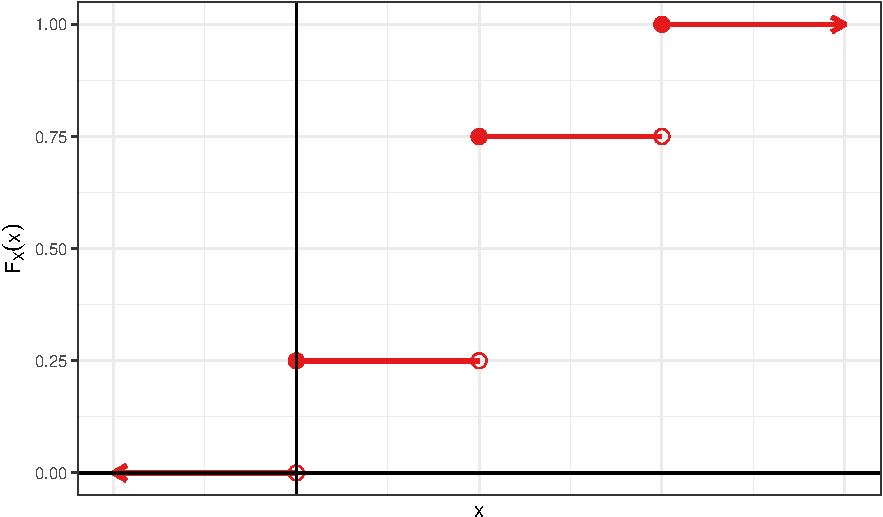
\includegraphics{00-prelim_files/figure-pdf/fig-eg-cdf-coin-flip-plot-1.pdf}

}

\caption{\label{fig-eg-cdf-coin-flip-plot}The cdf for the two coin flip
example.}

\end{figure}%

Note that a cdf completely determines the distribution of a random
variable. This statement is captured in
Theorem~\ref{thm-cdf-determines-dist}.

\begin{theorem}[]\protect\hypertarget{thm-cdf-determines-dist}{}\label{thm-cdf-determines-dist}

Let \(X\) have cdf \(F\) and \(Y\) have cdf \(G\). If \(F(x) = G(x)\)
for all \(x,\) then \(P(X \in A)= P(Y \in A) \forall A \in \mathbf{R}\).

\end{theorem}

Since cdfs determine or characterize a probability distribution, it is
useful to know the key properties of cdfs, which are listed below in
Theorem~\ref{thm-cdf-properties}.

\begin{theorem}[Properties of
cdfs]\protect\hypertarget{thm-cdf-properties}{}\label{thm-cdf-properties}

\(F : \mathbf{R} \to [0,1]\) is a cdf for some \(P\) iff,

\begin{enumerate}
\def\labelenumi{\arabic{enumi}.}
\tightlist
\item
  \(F\) is nondecreasing (i.e.,
  \(x_1 < x_2 \implies F(x_1) \leq F(x_2)\)),
\item
  \(F\) is normalized to \([0,1]\) (i.e.,
  \(\lim_{x \to -\infty} F(x) = 0\) and
  \(\lim_{x \to \infty} F(x) = 1\)),
\item
  \(F\) is right-continuous (i.e., \(F(x) = F(x^*) \forall x\) where
  \(F(x^*) = \lim_{y > x; y \to x} F(y)\)).
\end{enumerate}

\end{theorem}

For a rv \(X\) we say \(X\) is \emph{discrete} if it assumes at most a
\emph{countable} number of (discrete) values. For a discrete sample
space, the collection of all probabilities of \(X(\omega)\) gives us a
probability distribution.

\begin{definition}[Pmf]\protect\hypertarget{def-pmf}{}\label{def-pmf}

A pdf for a discrete rv \(X\) is \(f_X(x) = P(X = x)\). Since this
density function places a ``point mass'' at each \(x,\) it is sometimes
referred to as a probability mass function (pmf).

\end{definition}

Figure~\ref{fig-eg-pmf-histogram} displays the pmf for the coin flip
experiment considered in Example~\ref{exm-rv-3}. The pmf is a histogram
with point masses at \(x = 0,\) \(x=1,\) and \(x=2\). The mass placed at
these points is given by \(P(X = x)\). Since the pmf is a pdf for a
discrete random variable, recall from the axioms of probability that the
pmf therefore satisfies \(f(x) \geq 0,\) \(\forall x \in \mathbf{R},\)
and \(\sum_i f(x_i) = 1\). This fact can be observed in
Figure~\ref{fig-eg-pmf-histogram}:
\(f_X(0) + f_X(1) + f_X(2) = 0.25 + 0.5 + 0.25 = 1\).

\begin{figure}

\centering{

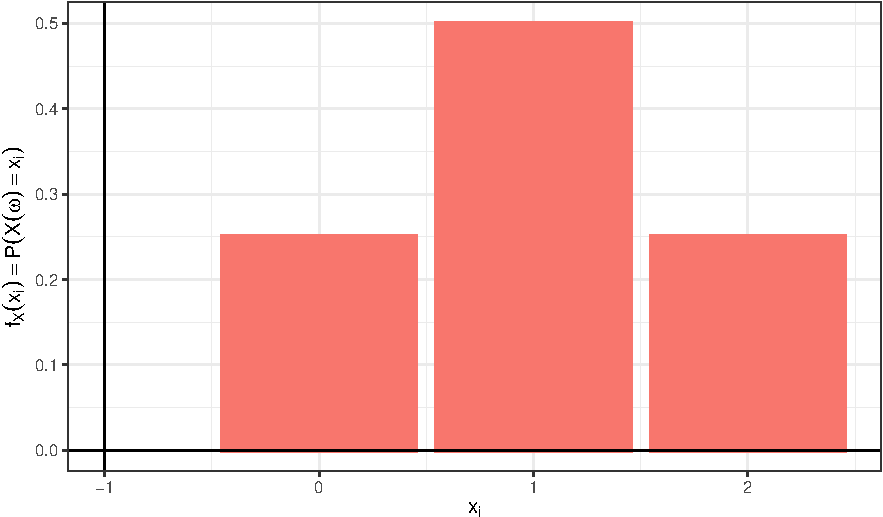
\includegraphics{00-prelim_files/figure-pdf/fig-eg-pmf-histogram-1.pdf}

}

\caption{\label{fig-eg-pmf-histogram}The histogram (pmf) for the two
coin flip example.}

\end{figure}%

A rv \(X\) is \emph{continuous} if there exists a continuous function
\(f_X\) such that,

\begin{enumerate}
\def\labelenumi{\arabic{enumi}.}
\tightlist
\item
  \(f_X(x) \geq 0 \forall x,\)
\item
  \(\int_{-\infty}^\infty f_X(x) dx = 1\) and
\item
  \(P(a < X < b) = \int_a^b f_X(x) dx,\) for \(a\leq b\).
\end{enumerate}

\begin{definition}[Pdf]\protect\hypertarget{def-pdf}{}\label{def-pdf}

A \(f_X\) satisfying the three properties above is a pdf for the
continous rv \(X\).

\end{definition}

\begin{tcolorbox}[enhanced jigsaw, toprule=.15mm, leftrule=.75mm, colframe=quarto-callout-important-color-frame, arc=.35mm, rightrule=.15mm, bottomrule=.15mm, coltitle=black, title=\textcolor{quarto-callout-important-color}{\faExclamation}\hspace{0.5em}{Events of probability zero}, breakable, colbacktitle=quarto-callout-important-color!10!white, bottomtitle=1mm, left=2mm, toptitle=1mm, titlerule=0mm, opacityback=0, opacitybacktitle=0.6, colback=white]

If \(X\) is continuous, then \(P(X = x) = 0\) for every \(x\). That is,
\[ 
P(a \leq X \leq b) = P(a < X \leq b) = P(a \leq X < b) = P(a < X < b),.
\]

\end{tcolorbox}

The cdf is related to the pdf by the derivative (difference). If \(X\)
is continuous: \[ F_X(x) = P(X \leq x) = \int_{-\infty}^x f_X(t) dt\]
and \(f_X(x) = F_X^\prime(x)\) at all \(x\) at which \(F_X\) is
differentiable. (Likewise, if \(X\) is discrete, then we replace the
integral with a sum
\(F_X(x) = P(X \leq x) = \sum_{x_i \leq x} f_X(x_i)\).)

\begin{definition}[Quantile
function]\protect\hypertarget{def-quantile}{}\label{def-quantile}

Let \(X\) be a rv with cdf \(F\). The inverse cdf, or quantile function,
is defined by \[F^{-1}(q) = \inf \{x : F(x) > q\}\] for \(q \in [0,1]\).
If \(F\) is monotonic increasing and continuous then \(F^{-1}(q)\) is
the unique real number \(x\) such that \(F(x) = q\).

\end{definition}

Some quantiles get used more than others (and therefore get names).
Important quantiles include, \(F^{-1}(\frac{1}{4})\) is the first
quantile, \(F^{-1}(\frac{1}{2})\) is the median, and
\(F^{-1}(\frac{3}{4})\) is the third quantile.

\begin{definition}[Equality in
distribution]\protect\hypertarget{def-equal-dist}{}\label{def-equal-dist}

We say \(X\) and \(Y\) are equal in distribution, \(X \equiv Y,\) if
\(F_X(x) = F_Y(x)\) for all \(x\).

\end{definition}

\begin{tcolorbox}[enhanced jigsaw, toprule=.15mm, leftrule=.75mm, colframe=quarto-callout-important-color-frame, arc=.35mm, rightrule=.15mm, bottomrule=.15mm, coltitle=black, title=\textcolor{quarto-callout-important-color}{\faExclamation}\hspace{0.5em}{Equality in distribution versus equality of rvs}, breakable, colbacktitle=quarto-callout-important-color!10!white, bottomtitle=1mm, left=2mm, toptitle=1mm, titlerule=0mm, opacityback=0, opacitybacktitle=0.6, colback=white]

Note that equality in distribution does not mean that the random
variables are the same. Rather, probability statements are the same.

Consider the following example. Suppose
\[P(X = 1) = P(X = -1) = \frac{1}{2}\,.\] Let \(Y = -X\). Then
\[P(Y = 1) = P(Y = -1) = \frac{1}{2}\,.\] Thus, \[X \equiv Y \,,\] but
\(X\) and \(Y\) are not equal! In fact, \(P(X = Y) = 0\).

\end{tcolorbox}

We sometimes consider more than one random variable, taken to together.
This leads to the concept of a joint and marginal densities.

\begin{definition}[Joint
pdf]\protect\hypertarget{def-joint-pdf}{}\label{def-joint-pdf}

A joint pdf for \((X,Y)\) satisfies

\begin{enumerate}
\def\labelenumi{\arabic{enumi}.}
\tightlist
\item
  \(f(x,y) \geq 0\) \(\forall x,y,\)
\item
  \(\iint_{-\infty}^\infty f(x,y) dx dy = 1,\)
\item
  for \(A \in \mathbf{R}\times \mathbf{R},\)
  \(P((X,Y) \in A) = \iint_A f(x,y) dx dy\).
\end{enumerate}

\end{definition}

\begin{definition}[Joint
cdf]\protect\hypertarget{def-joint-cdf}{}\label{def-joint-cdf}

A joint cdf is given by \(F(x,y) = P(X\leq x, Y\leq y)\).

\end{definition}

\begin{definition}[marginal
pdf]\protect\hypertarget{def-marginals}{}\label{def-marginals}

For \(X,Y\) with joint pdf \(f(x,y),\) we define the marginals for \(X\)
and \(Y\) as \(f_X(x) \int f(x,y) dy\) and \(f_Y(y) = \int f(x,y) dx,\)
respectively.

\end{definition}

We also have a notion of independence for two rvs.

\begin{definition}[Independence of
rvs]\protect\hypertarget{def-indep-rv}{}\label{def-indep-rv}

Rvs \(X\) and \(Y\) are independent if
\(P(X \in A, Y \in B) = P(X \in A) P(Y \in B)\).

\end{definition}

\begin{theorem}[]\protect\hypertarget{thm-pdf-indep-rv}{}\label{thm-pdf-indep-rv}

Let \(X,Y\) have joint \(f_{XY}\). Then \(X\) and \(Y\) are independent
iff \(f_{XY} = f_X \cdot f_Y\) for all \(x,y\).

\end{theorem}

If \(X_1, \dots X_n\) are independent and each as the same marginal
distribution with cdf \(F,\) we say \(X_1, \dots, X_n\) are iid and
write \(X_1, \dots, X_n \sim F\) iid. We also write
\(X_1, \dots, X_n \sim f\) if \(F\) has corresponding density \(f,\)
when no confusion arises. We will often consider collections of iid
random variables.

\begin{definition}[Random
sample]\protect\hypertarget{def-sample}{}\label{def-sample}

\(X_1, \dots, X_n \sim F\) iid is a random sample of size \(n\) from a
distribution \(F\).

\end{definition}

We also consider the expected value of a rv.

\begin{definition}[Expectation]\protect\hypertarget{def-expected-value}{}\label{def-expected-value}

For a discrete rv \(X\) with possible outcomes \(x_1, x_2, \dots\) and
corresponding probabilities \(p_1, p_2, \dots,\) the expectation is
defined by \[\mathbf{E}[X] = \sum_{i=1}^\infty x_i p_i\,.\]

For a continuous rv \(X\) with pdf \(f,\) the expectation is defined by
\[\mathbf{E}[X] = \int_{-\infty}^{\infty} x f(x) dx\,.\]

\end{definition}

For both discrete and continuous rvs, we refer to various statistics
relating to expected values as moments of the distribution.

\begin{definition}[\(n\)-th raw
moment]\protect\hypertarget{def-raw-moments}{}\label{def-raw-moments}

For a rv \(X,\) the \(n\)-th raw moment is given by \(\mathbf{E}[X^n]\).

\end{definition}

\begin{definition}[\(n\)-th central
moment]\protect\hypertarget{def-central-moments}{}\label{def-central-moments}

For a rv \(X\) with \(\mu = \mathbf{E}[X],\) the \(n\)-th central moment
is defined as \(\mathbf{E}[(X-\mu)^n]\).

\end{definition}

The \emph{mean} of a distribution is the first raw moment. The
\emph{variance} of a distribution is the second central moment.
Quantities related to higher order central moments are also of interest;
Table~\ref{tbl-moments} lists some of these with associated ``names''
that you might encounter. Variance is a measure of dispersion about the
mean. Skewness is a measure of the lopsidedness of a distribution. If a
distribution is symmetric (and its third central moment is defined) then
it will have skewness equal to zero. A distribution that is skewed to
the left (i.e., the tail of the distribution is longer on the left) will
have negative skewness and a distribution that is skewed to the right
(i.e., the tail of the distribution is longer on the right) will have
positive skewness. Kurtosis is a measure of how ``fat'' or ``heavy'' the
tails of a distribution are; distributions with heavy tails will have
high kurtosis values. Since variance and kurtosis are related to the
even-powered central moments, they will always be non-negative.

\begin{table}

\caption{\label{tbl-moments}First few moments for a rv \(X\) with mean
\(\mu = \mathbf{E}[X]\).}

\begin{minipage}{0.50\linewidth}

\subcaption{\label{tbl-raw-moments}Quantities related to raw moments}

\centering{

\begin{tabular}{cc}
\toprule
Expression & Name\\
\midrule
\(\mathbf{E}[X]\) & mean\\
\(\mathbf{E}[X^2]\) & ---\\
\(\mathbf{E}[X^3]\) & ---\\
\(\mathbf{E}[X^4]\) & ---\\
\bottomrule
\end{tabular}

}

\end{minipage}%
%
\begin{minipage}{0.50\linewidth}

\subcaption{\label{tbl-central-moments}Quantities related to central
moments}

\centering{

\begin{tabular}{cc}
\toprule
Expression & Name\\
\midrule
\(\mathbf{E}[(X - \mu)]\) & ---\\
\(\mathbf{E}[(X - \mu)^2]\) & variance\\
\(\mathbf{E}[(X - \mu)^3 / \sigma^3]\) & (Fisher's) skewness\\
\(\mathbf{E}[(X - \mu)^4 / \sigma^4]\) & kurtosis\\
\bottomrule
\end{tabular}

}

\end{minipage}%

\end{table}%

\begin{tcolorbox}[enhanced jigsaw, toprule=.15mm, leftrule=.75mm, colframe=quarto-callout-note-color-frame, arc=.35mm, rightrule=.15mm, bottomrule=.15mm, coltitle=black, title=\textcolor{quarto-callout-note-color}{\faInfo}\hspace{0.5em}{Its all Greek \ldots{} when it comes to kurtosis}, breakable, colbacktitle=quarto-callout-note-color!10!white, bottomtitle=1mm, left=2mm, toptitle=1mm, titlerule=0mm, opacityback=0, opacitybacktitle=0.6, colback=white]

The root of kurtosis comes from the Greek word for ``bulging'' or
``convex''. You may see a heavy-tailed or high kurtosis distributions
described as \emph{leptokurtic} (``narrow'' + ``bulging'') and a
light-tailed or low kurtosis distributions described as
\emph{platykurtic} (``broad'' or ``flat'' + ``bulging''). The ``high''
and ``low'' qualifications are made in relation to the tails of the
normal distribution; a distribution having the same kurtosis as the
normal distribution can be described as \emph{mesokurtic} (``middle'' +
``bulging'').

\end{tcolorbox}

\chapter{Sampling distributions}\label{sec-sampling-distributions}

A \emph{statistic} is a quantity that can be calculated from sample
data. Before observing data, a statistic is an unknown quantity and is,
therefore, a rv.

\begin{definition}[Statistic]\protect\hypertarget{def-statistic}{}\label{def-statistic}

Let \(X_1, \dots, X_n\) be observable rvs and let \(g\) be an arbitrary
real-valued function of \(n\) random variables. The rv
\[T = g(X_1, \dots, X_n)\] is a statistic.

\end{definition}

We refer to the probability distribution for a statistic as a sampling
distribution. The sampling distribution illustrates how the statistic
will vary across possible sample data. The sampling distribution
contains information about the values a statistic is likely to assume
and how likely it is to assume those values prior to observing data.

\begin{definition}[Sampling
distribution]\protect\hypertarget{def-sampling-dist}{}\label{def-sampling-dist}

Suppose rvs \(X_1, \dots, X_n\) are a random sample from \(F(\theta),\)
a distribution depending a parameter \(\theta\) whose value is uknown.
Let the rv \[T = g(X_1, \dots, X_n, \theta)\] be a function of
\(X_1, \dots, X_n\) and (possibly) \(\theta\). The distribution of \(T\)
(given \(\theta\)) is the sampling distribution of \(T\).

\end{definition}

The sampling distribution of \(T\) is derived from the distribution of
the random sample. Often we will be interested in a statistic \(T\) that
is an estimator for a parameter \(\theta\) (that is, \(T\) will not
depend on \(\theta\)).

In what follows, we review several special families of distributions
that are widely used in probability and statistics. These special
families of distributions will be indexed by one or parameters.

\section{Uniform distribution}\label{sec-uniform-distribution}

The uniform distribution places equal on uniform weight on the items
being sampled.

\begin{definition}[Uniform
distribution]\protect\hypertarget{def-uniform-dist}{}\label{def-uniform-dist}

A continuous rv \(X\) has a uniform distribution on \([a,b]\) with
\(a<b,\) if \(X\) has pdf \[
 f(x; a,b) = \frac{1}{b-a}\,, 
 \quad a < x < b\,,
\] or zero otherwise. We write \(X \sim \mathsf{Unif}(a,b)\).

\end{definition}

\begin{tcolorbox}[enhanced jigsaw, toprule=.15mm, leftrule=.75mm, colframe=quarto-callout-warning-color-frame, arc=.35mm, rightrule=.15mm, bottomrule=.15mm, coltitle=black, title=\textcolor{quarto-callout-warning-color}{\faExclamationTriangle}\hspace{0.5em}{Parameters}, breakable, colbacktitle=quarto-callout-warning-color!10!white, bottomtitle=1mm, left=2mm, toptitle=1mm, titlerule=0mm, opacityback=0, opacitybacktitle=0.6, colback=white]

Note that \(a\) and \(b\) are parameters in
Definition~\ref{def-uniform-dist}.

\end{tcolorbox}

\begin{exercise}[]\protect\hypertarget{exr-uniform}{}\label{exr-uniform}

As an exercise, derive the cdf using the definition. Derive a formula
for the mean and variance in terms of the parameters \(a\) and \(b\).

\end{exercise}

\section{Normal distribution}\label{sec-normal-distribution}

Normal distributions play an important role in probability and
statistics as they describe many natural phenomena. For instance, the
Central Limit Theorem tells us that the sample mean of a large random
sample (size \(m\)) of rvs with mean \(\mu\) and variance \(\sigma^2\)
is approximately normal in distribution with mean \(\mu\) and variance
\(\sigma^2/m\).

\begin{definition}[Normal or Gaussian
distribution]\protect\hypertarget{def-normal-dist}{}\label{def-normal-dist}

A continuous rv \(X\) has a normal distribution with parameters \(\mu\)
and \(\sigma^2,\) where \(-\infty < \mu < \infty\) and \(\sigma > 0,\)
if \(X\) has pdf \[
 f(x; \mu, \sigma) = \frac{1}{\sqrt{2 \pi} \sigma}e^{-(x-\mu)^2/(2\sigma^2)}\,, 
 \quad -\infty < x < \infty \,.
\] We write \(X \sim \mathsf{N}(\mu, \sigma^2)\).

\end{definition}

For \(X\sim \mathsf{N}(\mu,\sigma^2),\) it can be shown that
\(\mathbf{E}(X) = \mu\) and \(\mathop{\mathrm{Var}}(X) = \sigma^2,\)
that is, \(\mu\) is the \emph{mean} and \(\sigma^2\) is the
\emph{variance} of \(X\). The pdf forms a bell-shaped curve that is
symmetric about \(\mu,\) as illustrated in
Figure~\ref{fig-normals-diff-mean}. The value \(\sigma\) (\emph{standard
deviation}) is the distance from \(\mu\) to the inflection points of the
curve. As \(\sigma\) increases, the dispersion in the density increases,
as illustrated in Figure~\ref{fig-normals-diff-sd}. Thus, the
distribution's position (location) and spread depend on \(\mu\) and
\(\sigma\).

\begin{figure}

\centering{

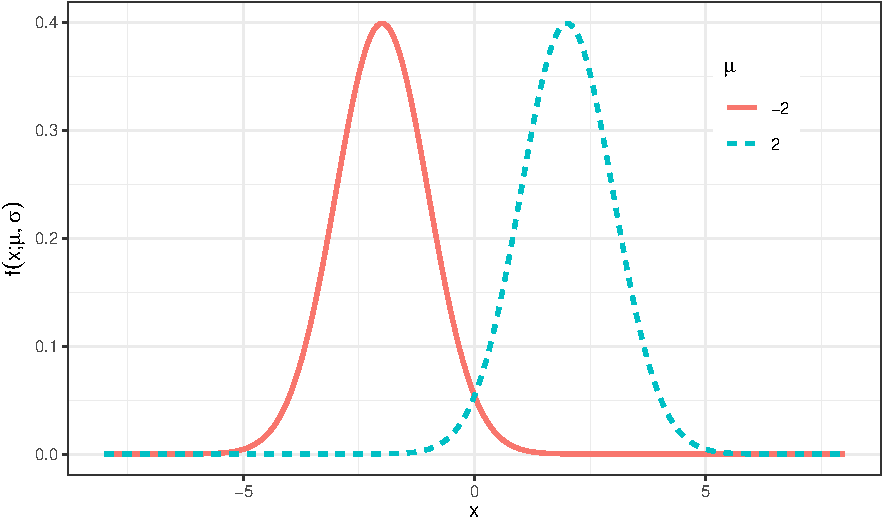
\includegraphics{01-sampling-distributions_files/figure-pdf/fig-normals-diff-mean-1.pdf}

}

\caption{\label{fig-normals-diff-mean}The pdfs of two normal rvs,
\(X_1 \sim \mathsf{N}(-2, 1)\) and \(X_2 \sim \mathsf{N}(2, 1),\) with
\emph{different means} and the same standard deviations.}

\end{figure}%

\begin{figure}

\centering{

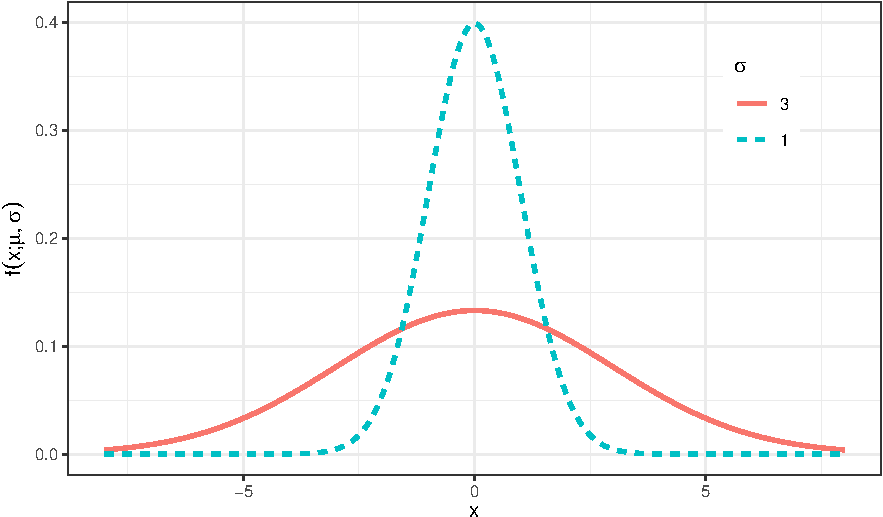
\includegraphics{01-sampling-distributions_files/figure-pdf/fig-normals-diff-sd-1.pdf}

}

\caption{\label{fig-normals-diff-sd}The pdfs of two normal rvs,
\(X_1 \sim \mathsf{N}(0, 9)\) and \(X_2 \sim \mathsf{N}(0, 1),\) with
the same means and \emph{different standard deviations}.}

\end{figure}%

\begin{definition}[Standard normal
distribution]\protect\hypertarget{def-standard-normal}{}\label{def-standard-normal}

We say that \(X\) has a standard normal distribution if \(\mu=0\) and
\(\sigma = 1\) and we will usually denote standard normal rvs by
\[Z \sim \mathsf{N}(0,1)\] (why \(Z\)? tradition!\footnote{``Traditions,
  traditions\ldots{} Without our traditions, our lives would be as shaky
  as a fiddler on the roof!''
  {[}\url{https://www.youtube.com/watch?v=gRdfX7ut8gw}{]}.}). We denote
the cdf of the standard normal by \[\Phi(z) = P(Z \leq z)\] and write
\(\varphi = \Phi'\) for its density function.

\end{definition}

\begin{tcolorbox}[enhanced jigsaw, toprule=.15mm, leftrule=.75mm, colframe=quarto-callout-important-color-frame, arc=.35mm, rightrule=.15mm, bottomrule=.15mm, coltitle=black, title=\textcolor{quarto-callout-important-color}{\faExclamation}\hspace{0.5em}{Useful facts about normal variates}, breakable, colbacktitle=quarto-callout-important-color!10!white, bottomtitle=1mm, left=2mm, toptitle=1mm, titlerule=0mm, opacityback=0, opacitybacktitle=0.6, colback=white]

\begin{enumerate}
\def\labelenumi{\arabic{enumi}.}
\tightlist
\item
  If \(X \sim \mathsf{N}(\mu, \sigma^2),\) then
  \[Z = (X - \mu) / \sigma  \sim \mathsf{N}(0,1).\]
\item
  If \(Z \sim \mathsf{N}(0, 1),\) then
  \[X = \mu + \sigma Z \sim \mathsf{N}(\mu, \sigma^2).\]
\item
  If \(X_i \sim \mathsf{N}(\mu_i, \sigma_i^2)\) for \(i = 1, \dots, n\)
  are independent rvs, then
  \[\sum_{i=1}^{n} X_i \sim \mathsf{N} \left( \sum_{i=1}^{n} \mu_i, \sum_{i=1}^{n} \sigma_i^2 \right) \,.\]\\
\end{enumerate}

\end{tcolorbox}

\begin{tcolorbox}[enhanced jigsaw, toprule=.15mm, leftrule=.75mm, colframe=quarto-callout-warning-color-frame, arc=.35mm, rightrule=.15mm, bottomrule=.15mm, coltitle=black, title=\textcolor{quarto-callout-warning-color}{\faExclamationTriangle}\hspace{0.5em}{Variances add}, breakable, colbacktitle=quarto-callout-warning-color!10!white, bottomtitle=1mm, left=2mm, toptitle=1mm, titlerule=0mm, opacityback=0, opacitybacktitle=0.6, colback=white]

In particular, for differences of independent rvs
\(X_1 \sim \mathsf{N}(\mu_1, \sigma_1^2)\) and
\(X_2 \sim \mathsf{N}(\mu_2, \sigma_2^2)\) then the variances add:
\[ X_1 - X_2 \sim \mathsf{N}(\mu_1 - \mu_2, \sigma_1^2 + \sigma_2^2) \,.\]

\end{tcolorbox}

Probabilities \(P(a \leq X \leq b)\) are found by converting the problem
in \(X \sim \mathsf{N}(\mu, \sigma^2)\) to the \emph{standard normal}
distribution \(Z \sim \mathsf{N}(0, 1)\) whose probability values
\(\Phi(z) = P(Z\leq z)\) can then be looked up in a table. From (1.)
above, \[
\begin{aligned}
   P(a < X < b) &= P\left( \frac{a-\mu}{\sigma} < Z < \frac{b-\mu}{\sigma} \right) \\ 
    &= \Phi \left( \frac{b-\mu}{\sigma}\right) - \Phi\left(\frac{a-\mu}{\sigma}\right) \,.
\end{aligned}
\] This process is often referred to as \emph{standardising} (the normal
rv).

\begin{example}[]\protect\hypertarget{exm-norm-rt}{}\label{exm-norm-rt}

Let \(X \sim \mathsf{N}(5, 9)\) and find \(P(X \geq 5.5)\).

\[
\begin{aligned}
   P(X \geq 5.5) &= P\left(Z \geq \frac{5.5 - 5}{3}\right) \\
    &= P(Z \geq 0.1667) \\
    &= 1 - P(Z \leq 0.1667) \\
    &= 1 - \Phi(0.1667) \\
    &= 1 - 0.5662 \\
    &= 0.4338\,,
\end{aligned}
\] where we look up the value of \(\Phi(z) = P(Z\leq z)\) in a table of
standard normal curve areas.

The probability corresponds to the shaded area under the normal density
\(\varphi(x) = \Phi'(x)\) corresponding to \(x \geq 5.5\) (see
Figure~\ref{fig-example-norm-geq}). To calculate this area, we can also
use the \texttt{R} code:
\texttt{pnorm(5.5,\ mean\ =\ 5,\ sd\ =\ 3,\ lower.tail\ =\ FALSE)}.

\begin{figure}

\centering{

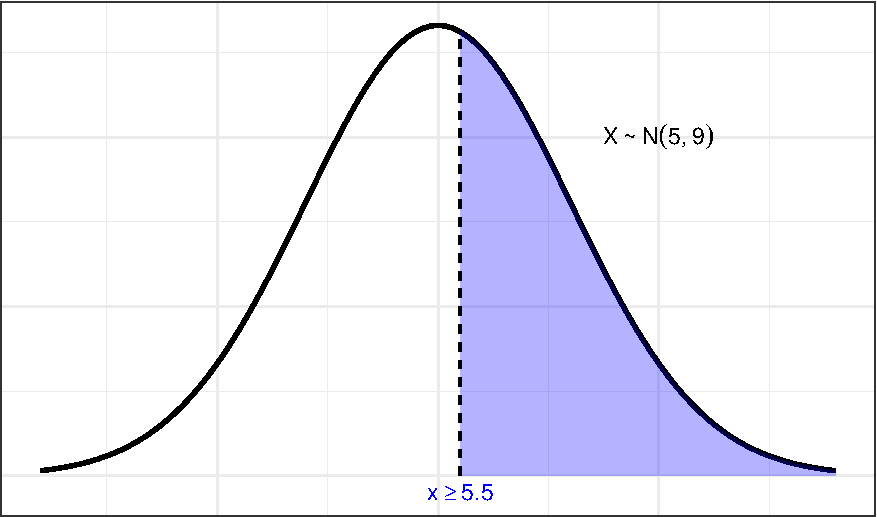
\includegraphics{01-sampling-distributions_files/figure-pdf/fig-example-norm-geq-1.pdf}

}

\caption{\label{fig-example-norm-geq}The normal density
\(\mathsf{N}(5,9)\) with the (one-sided) interval shaded in blue that
corresponds to the probability \(P(X \geq 5.5)\).}

\end{figure}%

\end{example}

\begin{example}[]\protect\hypertarget{exm-norm-dt}{}\label{exm-norm-dt}

Let \(X \sim \mathsf{N}(5, 9)\) and find \(P(4 \leq X \leq 5.25)\).

\[
\begin{aligned}
   P(4 \leq X \leq 5.25) &= P\left(\frac{4-5}{3} \leq Z \leq \frac{5.25-5}{3}\right) \\
   &= P(-0.3333 \leq Z \leq 0.0833) \\
   &= \Phi(0.0833) - \Phi(-0.3333) \\
   &= 0.5332 - 0.3694 \\
   &= 0.1638\,.
  \end{aligned}
\] where we look up the value of \(\Phi(z) = P(Z\leq z)\) in a table of
standard normal curve areas.

The probability corresponds to the shaded area under the normal density
\(\varphi(x) = \Phi'(x)\) corresponding to \(4 \leq x \leq 5.25\) (see
Figure~\ref{fig-example-norm-interval}). To calculate this area, we can
use the \texttt{R} code:
\texttt{pnorm(5.25,\ mean\ =\ 5,\ sd\ =\ 3)\ -\ pnorm(4,\ mean\ =\ 5,\ sd\ =\ 3)}.

\begin{figure}

\centering{

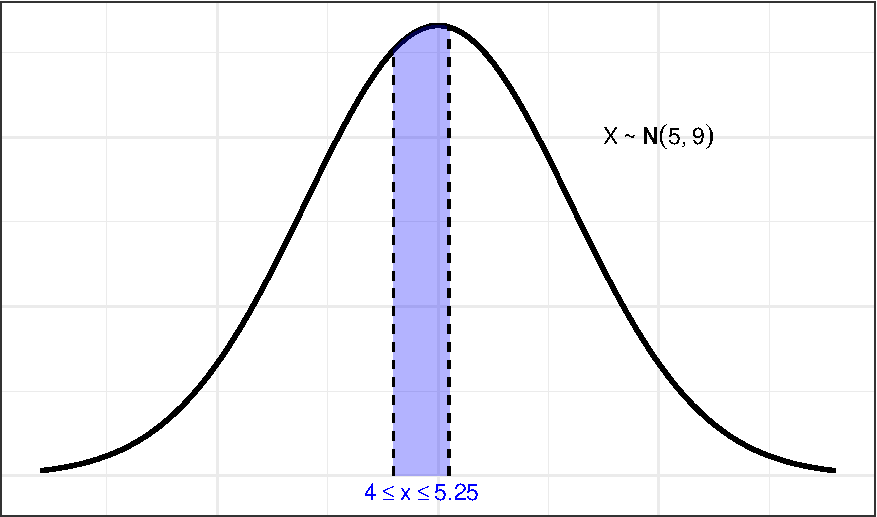
\includegraphics{01-sampling-distributions_files/figure-pdf/fig-example-norm-interval-1.pdf}

}

\caption{\label{fig-example-norm-interval}The normal density
\(\mathsf{N}(5,9)\) with the (two-sided) interval shaded in blue that
corresponds to the probability \(P(4 \leq X \leq 5.25)\).}

\end{figure}%

\end{example}

\begin{tcolorbox}[enhanced jigsaw, toprule=.15mm, leftrule=.75mm, colframe=quarto-callout-important-color-frame, arc=.35mm, rightrule=.15mm, bottomrule=.15mm, coltitle=black, title=\textcolor{quarto-callout-important-color}{\faExclamation}\hspace{0.5em}{Empirical rule (\(68-95-99.7\) rule)}, breakable, colbacktitle=quarto-callout-important-color!10!white, bottomtitle=1mm, left=2mm, toptitle=1mm, titlerule=0mm, opacityback=0, opacitybacktitle=0.6, colback=white]

For samples from a normal distribution, the percentage of values that
lie within one, two, and three standard deviations of the mean are
\(68.27\%,\) \(95.45\%,\) and \(99.73\%,\) respectively. That is, for
\(X \sim \mathsf{N}(\mu, \sigma^2),\) \[
P(\mu - 1 \sigma \leq X \leq \mu + 1 \sigma ) \approx 0.6827\,,
\] \[
P(\mu - 2 \sigma \leq X \leq \mu + 2 \sigma ) \approx 0.9545\,,
\] \[
P(\mu - 3 \sigma \leq X \leq \mu + 3 \sigma ) \approx 0.9973\,.
\] For a normal population, nearly all the values lie within ``three
sigmas'' of the mean.

\end{tcolorbox}

\section{\texorpdfstring{Student's \(\mathsf{t}\)
distribution}{Student's \textbackslash mathsf\{t\} distribution}}\label{sec-t-distribution}

Student's \(\mathsf{t}\) distribution gets its peculiar name as it was
first published under the pseudonym ``Student''.\footnote{William Sealy
  Gosset (1876--1937) wrote under the pseudonym ``Student''
  {[}\url{https://mathshistory.st-andrews.ac.uk/Biographies/Gosset/}{]}.}
This bit of obfuscation was to protect the identity of his
employer,\footnote{Gosset invented the t-test to handle small samples
  for quality control in brewing, specifically for the Guinness brewery
  in Dublin {[}\url{https://www.wikiwand.com/en/Guinness_Brewery}{]}.}
and thereby vital trade secrets, in a highly competitive and lucrative
industry.

\begin{definition}[Student's \(\mathsf{t}\)
distribution]\protect\hypertarget{def-t-dist}{}\label{def-t-dist}

A continuous rv \(X\) has a \(\mathsf{t}\) distribution with parameter
\(\nu > 0,\) if \(X\) has pdf \[
f(x; \nu) = \frac{\Gamma\left(\tfrac{\nu+1}{2}\right)}{\sqrt{\nu \pi} \Gamma \left(\tfrac{\nu}{2}\right)} \left( 1 + \tfrac{x^2}{\nu} \right)^{- \frac{\nu+1}{2}} \,, \quad -\infty < x < \infty\,.
\] We write \(X \sim \mathsf{t}(\nu)\). Note \(\Gamma\) is the standard
gamma function.\footnote{The gamma function is defined by
  \(\Gamma(z) = \int_0^\infty x^{z-1}e^{-x} dx\) when the real part of
  \(z\) is positive. For any positive integer \(n,\)
  \(\Gamma(n) = (n-1)!\) and for half-integers
  \(\Gamma(\tfrac{1}{2} + n) = \frac{(2n)!}{4^n n!} \sqrt{\pi}\).}

\end{definition}

The density for \(\mathsf{t}(\nu)\) for several values of \(\nu\) are
plotted below in Figure~\ref{fig-example-t-dist}.

\begin{figure}

\centering{

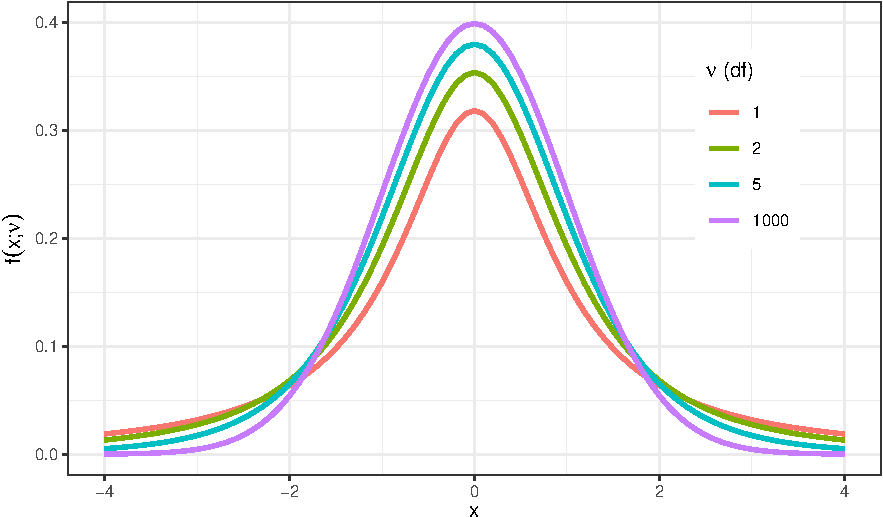
\includegraphics{01-sampling-distributions_files/figure-pdf/fig-example-t-dist-1.pdf}

}

\caption{\label{fig-example-t-dist}The density for \(\mathsf{t}(\nu)\)
for several values of \(\nu\) (df).}

\end{figure}%

\begin{tcolorbox}[enhanced jigsaw, toprule=.15mm, leftrule=.75mm, colframe=quarto-callout-important-color-frame, arc=.35mm, rightrule=.15mm, bottomrule=.15mm, coltitle=black, title=\textcolor{quarto-callout-important-color}{\faExclamation}\hspace{0.5em}{Properties of \(\mathsf{t}\) distributions}, breakable, colbacktitle=quarto-callout-important-color!10!white, bottomtitle=1mm, left=2mm, toptitle=1mm, titlerule=0mm, opacityback=0, opacitybacktitle=0.6, colback=white]

\begin{enumerate}
\def\labelenumi{\arabic{enumi}.}
\tightlist
\item
  The density for \(\mathsf{t}(\nu)\) is a bell-shaped curve centred at
  \(0\).
\item
  The density for \(\mathsf{t}(\nu)\) is more spread out than the
  standard normal density (i.e., it has ``fatter tails'' than the
  normal).
\item
  As \(\nu \to \infty,\) the spread of the corresponding
  \(\mathsf{t}(\nu)\) density converges to the standard normal density
  (i.e., the spread of the \(\mathsf{t}(\nu)\) density decreases
  relative to the standard normal).
\end{enumerate}

If \(X \sim \mathsf{t}(\nu),\) then \(\mathbf{E}[X] = 0\) for
\(\nu > 1\) (otherwise the mean is undefined).

\end{tcolorbox}

\begin{tcolorbox}[enhanced jigsaw, toprule=.15mm, leftrule=.75mm, colframe=quarto-callout-note-color-frame, arc=.35mm, rightrule=.15mm, bottomrule=.15mm, coltitle=black, title=\textcolor{quarto-callout-note-color}{\faInfo}\hspace{0.5em}{Cauchy distribution}, breakable, colbacktitle=quarto-callout-note-color!10!white, bottomtitle=1mm, left=2mm, toptitle=1mm, titlerule=0mm, opacityback=0, opacitybacktitle=0.6, colback=white]

A \(\mathsf{t}\) distributions with \(\nu = 1\) has pdf
\[f(x) = \frac{1}{\pi (1 + x^2)}\,,\] and we call this the Cauchy
distribution.

\end{tcolorbox}

\section{\texorpdfstring{\(\chi^2\)
distribution}{\textbackslash chi\^{}2 distribution}}\label{sec-chisq-distribution}

The \(\chi^2\) distribution arises as the distribution of a sum of the
squares of \(\nu\) independent standard normal rvs.

\begin{definition}[\(\chi^2\)
distribution]\protect\hypertarget{def-chisq-dist}{}\label{def-chisq-dist}

A continuous rv \(X\) has a \(\chi^2\) distribution with parameter
\(\nu \in \mathbf{N}_{>},\) if \(X\) has pdf \begin{equation*}
f(x; \nu) = \frac{1}{2^{\nu/2} \Gamma(\nu/2)} x^{(\nu/2)-1} e^{-x/2} \,, 
\end{equation*} with support \(x \in (0, \infty)\) if \(\nu=1,\)
otherwise \(x \in [0, \infty)\). We write \(X \sim \chi^2(\nu)\).

\end{definition}

The pdf \(f(x; \nu)\) of the \(\chi^2(\nu)\) distribution depends on a
positive integer \(\nu\) referred to as the df. The densities for
several values of \(\nu\) are plotted below in
Figure~\ref{fig-example-chisq-dist}. The density \(f(x;\nu)\) is
positively skewed, i.e., the right tail is longer, so the mass is
concentrated to the figure's left in
Figure~\ref{fig-example-chisq-dist}. The distribution becomes more
symmetric as \(\nu\) increases. We denote critical values of the
\(\chi^2(\nu)\) distribution by \(\chi^2_{\alpha, \nu}\).

\begin{figure}

\centering{

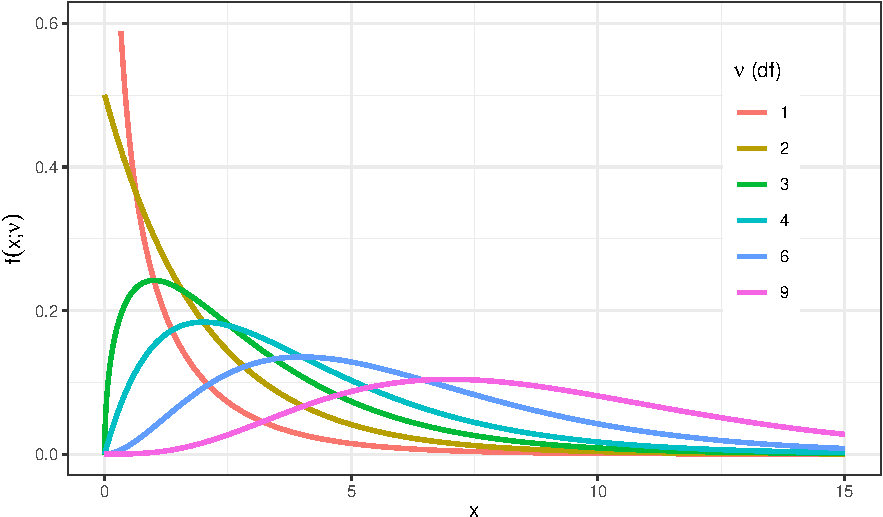
\includegraphics{01-sampling-distributions_files/figure-pdf/fig-example-chisq-dist-1.pdf}

}

\caption{\label{fig-example-chisq-dist}The density for \(\chi^2(\nu)\)
for several values of \(\nu\) (df).}

\end{figure}%

\begin{tcolorbox}[enhanced jigsaw, toprule=.15mm, leftrule=.75mm, colframe=quarto-callout-warning-color-frame, arc=.35mm, rightrule=.15mm, bottomrule=.15mm, coltitle=black, title=\textcolor{quarto-callout-warning-color}{\faExclamationTriangle}\hspace{0.5em}{Skew}, breakable, colbacktitle=quarto-callout-warning-color!10!white, bottomtitle=1mm, left=2mm, toptitle=1mm, titlerule=0mm, opacityback=0, opacitybacktitle=0.6, colback=white]

Unlike the normal and \(t\) distributions, the \(\chi^2\) distribution
is not symmetric! This means that critical values, e.g.,
\[\chi^2_{.99, \nu} \quad \text{and}\quad \chi^2_{0.01,\nu}\,,\] are
\textbf{not} equal. Hence, it will be necessary to look up both values
for CIs based on \(\chi^2\) critical values.

\end{tcolorbox}

If \(X \sim \chi^2(\nu),\) then \(\mathbf{E}[X] = \nu\) and
\(\mathop{\mathrm{Var}}[X] = 2\nu\).

\section{\texorpdfstring{\(\mathsf{F}\)
distribution}{\textbackslash mathsf\{F\} distribution}}\label{sec-F-distribution}

The \(\mathsf{F}\) distribution (``F'' for Fisher) arises as a test
statistic when comparing population variances and in the analysis of
variance (see @sec-anova).

\begin{definition}[\(\mathsf{F}\)
distribution]\protect\hypertarget{def-F-dist}{}\label{def-F-dist}

A continuous rv \(X\) has an \(\mathsf{F}\) distribution with df
parameters \(\nu_1\) and \(\nu_2,\) if \(X\) has pdf \[
 f(x; \nu_1, \nu_2) = 
    \frac{\Gamma\left(\frac{\nu_1+\nu_2}{2}\right) \nu_1^{\nu_1/2} \nu_2^{\nu_2/2}}
 {\Gamma\left(\frac{\nu_1}{2}\right) \Gamma\left(\frac{\nu_2}{2}\right)} 
 \frac{x^{\nu_1/2 - 1}}{(\nu_2+\nu_1 x)^{(\nu_1+\nu_2)/2}} \,.
\]

\end{definition}

The pdf \(f(x; \nu_1, \nu_2)\) of the \(\mathsf{F}(\nu_1, \nu_2)\)
distribution depends on two positive integers \(\nu_1\) and \(\nu_2\)
referred to, respectively, as the numerator and denominator df. The
density is plotted below for several combinations of \((\nu_1, \nu_2)\)
in Figure~\ref{fig-example-F-dist}.

\begin{figure}

\centering{

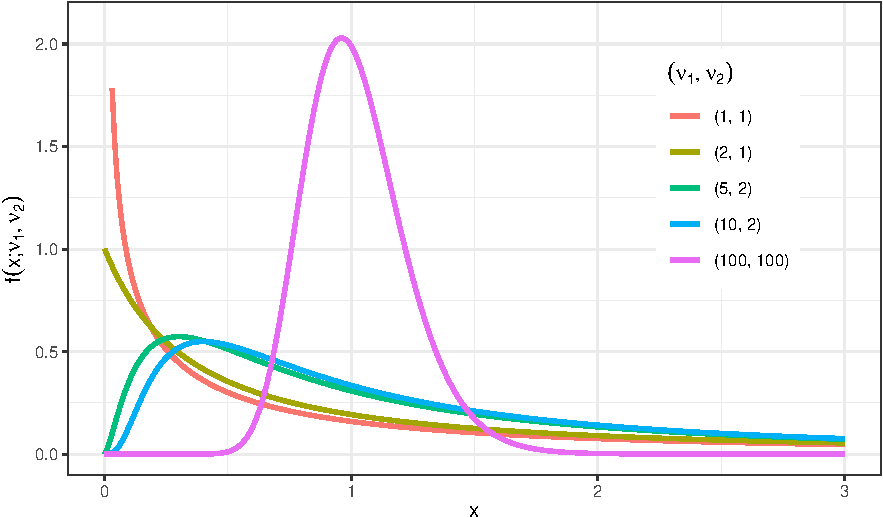
\includegraphics{01-sampling-distributions_files/figure-pdf/fig-example-F-dist-1.pdf}

}

\caption{\label{fig-example-F-dist}The density for
\(\mathsf{F}(\nu_1, \nu_2)\) for several combinations of
\((\nu_1, \nu_2)\).}

\end{figure}%

\begin{tcolorbox}[enhanced jigsaw, toprule=.15mm, leftrule=.75mm, colframe=quarto-callout-tip-color-frame, arc=.35mm, rightrule=.15mm, bottomrule=.15mm, coltitle=black, title=\textcolor{quarto-callout-tip-color}{\faLightbulb}\hspace{0.5em}{Where do the terms numerator and denominator df come from?}, breakable, colbacktitle=quarto-callout-tip-color!10!white, bottomtitle=1mm, left=2mm, toptitle=1mm, titlerule=0mm, opacityback=0, opacitybacktitle=0.6, colback=white]

The \(\mathsf{F}\) distribution is related to ratios of \(\chi^2\) rvs,
as captured in Theorem~\ref{thm-F-dist-chisq}.

\end{tcolorbox}

\begin{theorem}[Ratio of \(\chi^2\)
rvs]\protect\hypertarget{thm-F-dist-chisq}{}\label{thm-F-dist-chisq}

If \(X_1 \sim \chi^2(\nu_1)\) and \(X_2 \sim \chi^2(\nu_2)\) are
independent rvs, then the rv \[
 F = \frac{X_1 / \nu_1}{X_2 / \nu_2} \quad \sim \mathsf{F}(\nu_1,\nu_2)\,,
\] that comprises the ratio of two \(\chi^2\) rvs divided by their
respective df has an \(\mathsf{F}(\nu_1, \nu_2)\) distribution.

\end{theorem}

\chapter{Basics of statistical
inference}\label{sec-statistical-inference}

We discuss point estimation, confidence intervals, and hypothesis
testing in Sections Section~\ref{sec-point-estimation},
Section~\ref{sec-confidence-intervals}, and
Section~\ref{sec-hypothesis-testing}, respectively. These three tools
will form the basis for making inferences about a population.

\section{Point estimation}\label{sec-point-estimation}

Statistical inference seeks to draw conclusions about the
characteristics of a population from data. For example, suppose we are
botanists interested in the taxonomic classification of iris flowers.
Let \(\mu\) denote the true average petal length (in cm) of the
\emph{Iris setosa}\footnote{More about the \emph{Iris setosa} here
  {[}\url{https://www.wikiwand.com/en/Iris_setosa}{]}.} (AKA the
bristle-pointed iris). The parameter \(\mu\) is a characteristic of the
whole population of the \emph{setosa} species. Before we collect data,
the petal lengths of \(m\) independent \emph{setosa} flowers are denoted
by rvs \(X_1, X_2, \dots, X_m.\) Any function of the \(X_i\)'s, such as
the sample mean, \begin{equation}\phantomsection\label{eq-sample-mean}{
  \overline{X} = \frac{1}{m} \sum_{i=1}^m X_i\,, 
}\end{equation} or the sample variance,
\begin{equation}\phantomsection\label{eq-sample-var}{
  S^2 = \frac{1}{m-1} \sum_{i=1}^m (X_i - \overline{X})^2 \,, 
}\end{equation} is also a rv.

Suppose we actually find and measure the petal length of \(50\)
independent \emph{setosa} flowers resulting in observations
\(x_1, x_2, \dots, x_{50}\); the distribution (counts) of \(50\) such
petal length measurements are displayed in
Figure~\ref{fig-setosa-petal-lengths}. The sample mean \(\overline{x}\)
for petal length can then be used to draw a conclusion about the (true)
value of the population mean \(\mu.\) Based on the data in
Figure~\ref{fig-setosa-petal-lengths} and using
Equation~\ref{eq-sample-mean}, the value of the sample mean is
\(\overline{x} = 1.462.\) The value \(\overline{x}\) provides a ``best
guess'' or point estimate for the true value of \(\mu\) based on the
\(m=50\) samples.

\begin{figure}

\centering{

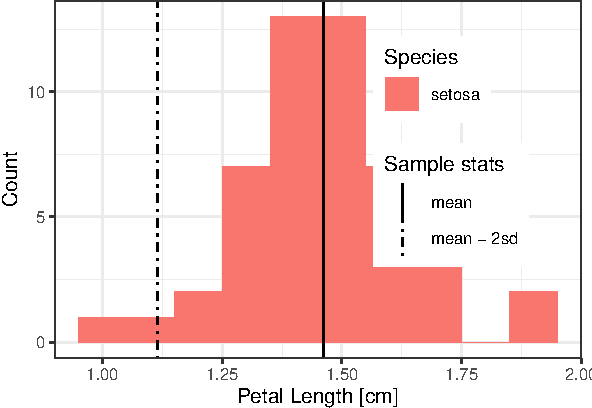
\includegraphics{02-basics-stat-infer_files/figure-pdf/fig-setosa-petal-lengths-1.pdf}

}

\caption{\label{fig-setosa-petal-lengths}The distribution (counts) of
\(m = 50\) \emph{setosa} petal length measurments.}

\end{figure}%

\begin{tcolorbox}[enhanced jigsaw, toprule=.15mm, leftrule=.75mm, colframe=quarto-callout-tip-color-frame, arc=.35mm, rightrule=.15mm, bottomrule=.15mm, coltitle=black, title=\textcolor{quarto-callout-tip-color}{\faLightbulb}\hspace{0.5em}{Loading datasets}, breakable, colbacktitle=quarto-callout-tip-color!10!white, bottomtitle=1mm, left=2mm, toptitle=1mm, titlerule=0mm, opacityback=0, opacitybacktitle=0.6, colback=white]

The \texttt{datasets} package has a variety of datasets that you can
play with. Once installed, data sets can be accessed in \texttt{R} by
loading \texttt{library(datasets)} and then calling, e.g.,
\texttt{data(iris)} to see the \texttt{iris} data set. For a full list
of available data sets, call \texttt{library(help\ =\ "datasets")} from
the console.

\end{tcolorbox}

\begin{tcolorbox}[enhanced jigsaw, toprule=.15mm, leftrule=.75mm, colframe=quarto-callout-note-color-frame, arc=.35mm, rightrule=.15mm, bottomrule=.15mm, coltitle=black, title=\textcolor{quarto-callout-note-color}{\faInfo}\hspace{0.5em}{Note \ref*{nte-iris}: Iris Data}, breakable, colbacktitle=quarto-callout-note-color!10!white, bottomtitle=1mm, left=2mm, toptitle=1mm, titlerule=0mm, opacityback=0, opacitybacktitle=0.6, colback=white]

\quartocalloutnte{nte-iris} 

The botanist Edgar Anderson's \textbf{Iris Data} contains 50 obs. of
four features (sepal length {[}cm{]}, sepal width {[}cm{]}, petal length
{[}cm{]}, and petal width {[}cm{]}) for each of three plant species
(\emph{setosa}, \emph{virginica}, \emph{versicolor}) for 150 obs. total.

\begin{Shaded}
\begin{Highlighting}[]
\NormalTok{iris }\SpecialCharTok{|\textgreater{}} \FunctionTok{glimpse}\NormalTok{()}
\end{Highlighting}
\end{Shaded}

\begin{verbatim}
Rows: 150
Columns: 5
$ Sepal.Length <dbl> 5.1, 4.9, 4.7, 4.6, 5.0, 5.4, 4.6, 5.0, 4.4, 4.9, 5.4, 4.8, 4.8, 4.~
$ Sepal.Width  <dbl> 3.5, 3.0, 3.2, 3.1, 3.6, 3.9, 3.4, 3.4, 2.9, 3.1, 3.7, 3.4, 3.0, 3.~
$ Petal.Length <dbl> 1.4, 1.4, 1.3, 1.5, 1.4, 1.7, 1.4, 1.5, 1.4, 1.5, 1.5, 1.6, 1.4, 1.~
$ Petal.Width  <dbl> 0.2, 0.2, 0.2, 0.2, 0.2, 0.4, 0.3, 0.2, 0.2, 0.1, 0.2, 0.2, 0.1, 0.~
$ Species      <fct> setosa, setosa, setosa, setosa, setosa, setosa, setosa, setosa, set~
\end{verbatim}

\end{tcolorbox}

\begin{definition}[Point
estimate]\protect\hypertarget{def-point-estimate}{}\label{def-point-estimate}

A point estimate of a parameter \(\theta\) (recall: a parameter is a
fixed, unknown quantity) is a single number that we consider a
reasonable value for \(\theta.\) Consider
\[\text{iid}\; X_1, X_2, \dots, X_m \sim F(\theta)\,.\] A point
estimator \(\widehat{\theta}_m\) of \(\theta\) is obtained by selecting
a suitable statistic \(g,\) \[
  \widehat{\theta}_m = g(X_1, \dots, X_m) \,.
\] A point estimate \(\widehat{\theta}_m\) can then be computed from the
estimator using sample data.

\end{definition}

\begin{tcolorbox}[enhanced jigsaw, toprule=.15mm, leftrule=.75mm, colframe=quarto-callout-warning-color-frame, arc=.35mm, rightrule=.15mm, bottomrule=.15mm, coltitle=black, title=\textcolor{quarto-callout-warning-color}{\faExclamationTriangle}\hspace{0.5em}{Overloaded notation}, breakable, colbacktitle=quarto-callout-warning-color!10!white, bottomtitle=1mm, left=2mm, toptitle=1mm, titlerule=0mm, opacityback=0, opacitybacktitle=0.6, colback=white]

The symbol \(\widehat{\theta}_m\) (or simply \(\widehat{\theta}\) when
the sample size \(m\) is clear from context) is typically used to denote
both the estimator and the point estimate resulting from a given sample.

\end{tcolorbox}

\begin{tcolorbox}[enhanced jigsaw, toprule=.15mm, leftrule=.75mm, colframe=quarto-callout-tip-color-frame, arc=.35mm, rightrule=.15mm, bottomrule=.15mm, coltitle=black, title=\textcolor{quarto-callout-tip-color}{\faLightbulb}\hspace{0.5em}{Best practice for reporting}, breakable, colbacktitle=quarto-callout-tip-color!10!white, bottomtitle=1mm, left=2mm, toptitle=1mm, titlerule=0mm, opacityback=0, opacitybacktitle=0.6, colback=white]

Writing, e.g., \(\widehat{\theta} = 42\) does not indicate how the point
estimate was obtained. Therefore, it is essential to report both the
estimator and the resulting point estimate.

\end{tcolorbox}

Definition~\ref{def-point-estimate} does not say how to select an
appropriate statistic. For the \emph{setosa} example, the sample mean
\(\overline{X}\) is suggested as a good estimator of the population mean
\(\mu.\) That is, \(\widehat{\mu} = \overline{X}\) or:

\begin{quote}
``the point estimator of \(\mu\) is the sample mean \(\overline{X}\)''.
\end{quote}

Here, while \(\mu\) and \(\sigma^2\) are fixed quantities representing
population characteristics, \(\overline{X}\) and \(S^2\) are rvs with
sampling distributions. If the population is \emph{normally distributed}
or if the \emph{sample is large} then the sampling distribution for
\(\overline{X}\) has a known form: \[
  \overline{X} \sim \mathsf{N}(\mu, \sigma^{2} / m) \,,
\] that is, \(\overline{X}\) is normal with mean
\(\mu_{\overline{X}} = \mu\) and variance
\(\sigma_{\overline{X}}^2 = \sigma^{2} / m\) where \(m\) is the sample
size and \(\mu\) and \(\sigma\) are the (typically unknown) population
parameters.

\begin{tcolorbox}[enhanced jigsaw, toprule=.15mm, leftrule=.75mm, colframe=quarto-callout-note-color-frame, arc=.35mm, rightrule=.15mm, bottomrule=.15mm, coltitle=black, title=\textcolor{quarto-callout-note-color}{\faInfo}\hspace{0.5em}{Note \ref*{nte-tree}: Cherry Tree Data}, breakable, colbacktitle=quarto-callout-note-color!10!white, bottomtitle=1mm, left=2mm, toptitle=1mm, titlerule=0mm, opacityback=0, opacitybacktitle=0.6, colback=white]

\quartocalloutnte{nte-tree} 

The \textbf{Cherry Tree Data} contains 31 obs. of three features
(diameter, height, and volume).

\begin{Shaded}
\begin{Highlighting}[]
\NormalTok{trees }\SpecialCharTok{|\textgreater{}} \FunctionTok{glimpse}\NormalTok{()}
\end{Highlighting}
\end{Shaded}

\begin{verbatim}
Rows: 31
Columns: 3
$ Girth  <dbl> 8.3, 8.6, 8.8, 10.5, 10.7, 10.8, 11.0, 11.0, 11.1, 11.2, 11.3, 11.4, 11.4~
$ Height <dbl> 70, 65, 63, 72, 81, 83, 66, 75, 80, 75, 79, 76, 76, 69, 75, 74, 85, 86, 7~
$ Volume <dbl> 10.3, 10.3, 10.2, 16.4, 18.8, 19.7, 15.6, 18.2, 22.6, 19.9, 24.2, 21.0, 2~
\end{verbatim}

\end{tcolorbox}

\begin{example}[]\protect\hypertarget{exm-estimators}{}\label{exm-estimators}

Let us consider the heights (measured in inches) of \(31\) black cherry
trees (sorted, for your enjoyment) in Table~\ref{tbl-cherry-data}.

\begin{table}

\caption{\label{tbl-cherry-data}Observations of \(m = 31\) felled black
cherry trees.}

\centering{

\centering
\begin{tabular}[t]{>{\raggedright\arraybackslash}p{150mm}}
\toprule
Height [in]\\
\midrule
\cellcolor{gray!10}{63, 64, 65, 66, 69, 70, 71, 72, 72, 74, 74, 75, 75, 75, 76, 76, 77, 78, 79, 80, 80, 80, 80, 80, 81, 81, 82, 83, 85, 86, 87}\\
\bottomrule
\end{tabular}

}

\end{table}%

\begin{figure}

\centering{

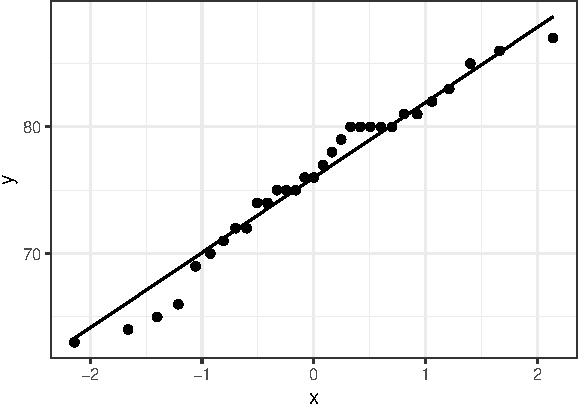
\includegraphics{02-basics-stat-infer_files/figure-pdf/fig-qq-plot-cherry-1.pdf}

}

\caption{\label{fig-qq-plot-cherry}Normal quantile-quantile plot for the
\texttt{Height} variable (feature) in the Cherry Tree Data.}

\end{figure}%

The quantile-quantile plot in Figure~\ref{fig-qq-plot-cherry}, which
compares the quantiles of this data to the quantiles of a normal
distribution, is fairly straight. Therefore, we assume that the
distribution of black cherry tree heights is (at least approximately)
normal with a mean value \(\mu\); i.e., that the population of heights
is distributed \(\mathsf{N}(\mu, \sigma^2),\) where \(\mu\) is a
parameter to be estimated and \(\sigma^2\) is unknown. The observations
\(X_1, \dots, X_{31}\) are then assumed to be a random sample from this
normal distribution, \[
\text{iid} \quad X_1, \dots, X_{31} \sim \mathsf{N}(\mu, \sigma^2) \,.
\]

Consider the following three different estimators and the resulting
point estimates for \(\mu\) based on the \(31\) samples in
Table~\ref{tbl-cherry-data}.

\begin{enumerate}
\def\labelenumi{\alph{enumi}.}
\item
  Estimator (sample mean) \(\overline{X}\) as in
  Equation~\ref{eq-sample-mean} and estimate
  \(\overline{x} = \sum x_i / n = 2356 / 31 = 76.\)
\item
  Estimator (average of extreme heights)
  \(\widetilde{X} = [\min(X_i) + \max(X_i)]/2\) and estimate
  \(\widetilde{x} = (63 + 87)/2 = 75.\)
\item
  Estimator (\(10\%\) trimmed mean -- i.e., in this instance exclude the
  smallest and largest three values) \(\overline{X}_{\text{tr}(10)}\)
  and estimate
  \(\overline{x}_{\text{tr}(10)} = (2356 - 63 - 64 - 65 - 87 - 86 - 85) / 25 = 76.24.\)
\end{enumerate}

Each estimator above uses a different notion of ``centre'' for the
sample data, i.e., represents a different statistic. An interesting
question is: which estimator will tend to produce estimates closest to
the true parameter value? Will the estimators work universally well for
all distributions?

\end{example}

\begin{tcolorbox}[enhanced jigsaw, toprule=.15mm, leftrule=.75mm, colframe=quarto-callout-tip-color-frame, arc=.35mm, rightrule=.15mm, bottomrule=.15mm, coltitle=black, title=\textcolor{quarto-callout-tip-color}{\faLightbulb}\hspace{0.5em}{How do we tell whether a population is normal?}, breakable, colbacktitle=quarto-callout-tip-color!10!white, bottomtitle=1mm, left=2mm, toptitle=1mm, titlerule=0mm, opacityback=0, opacitybacktitle=0.6, colback=white]

Constructing a normal quantile-quantile plot (or QQ plot) is one way of
assessing whether a normality assumption is reasonable. A QQ plot
compares the quantiles of the sample data \(x_i\) against the
theoretical standard normal quantiles, see
Figure~\ref{fig-qq-plot-cherry}. If the sample data is consistent with a
sample from a normal distribution, the points will lie in a straight
line (more or less). The QQ plot in Figure~\ref{fig-qq-plot-cherry}
compares quantiles of cherry tree heights from
Table~\ref{tbl-cherry-data} to normal quantiles. It is produced using
the following code.

\begin{Shaded}
\begin{Highlighting}[]
\NormalTok{trees }\SpecialCharTok{|\textgreater{}} \FunctionTok{ggplot}\NormalTok{(}\FunctionTok{aes}\NormalTok{(}\AttributeTok{sample =}\NormalTok{ Height)) }\SpecialCharTok{+} \FunctionTok{stat\_qq}\NormalTok{() }\SpecialCharTok{+} \FunctionTok{stat\_qq\_line}\NormalTok{()}
\end{Highlighting}
\end{Shaded}

The data \texttt{trees} is piped to the command \texttt{ggplot}. For a
QQ plot the key aesthetic element is \texttt{sample}; in this particular
instance we set this to \texttt{Height}. The geometry
\texttt{stat\_qq()} adds the data quantiles plotted versus the normal
quantiles. The geometry \texttt{stat\_qq\_line()} simply adds the fit
line.

\end{tcolorbox}

\begin{example}[]\protect\hypertarget{exm-infer-point-estimation}{}\label{exm-infer-point-estimation}

Although probably overkill for this problem, the \texttt{infer} package
can be used for point estimation using the \texttt{specify} and
\texttt{calculate} commands as follows:

\begin{Shaded}
\begin{Highlighting}[]
\NormalTok{trees }\SpecialCharTok{|\textgreater{}}
 \FunctionTok{specify}\NormalTok{(}\AttributeTok{response =}\NormalTok{ Height) }\SpecialCharTok{|\textgreater{}}
 \FunctionTok{calculate}\NormalTok{(}\AttributeTok{stat =} \StringTok{"mean"}\NormalTok{)}
\end{Highlighting}
\end{Shaded}

\begin{verbatim}
Response: Height (numeric)
# A tibble: 1 x 1
   stat
  <dbl>
1    76
\end{verbatim}

The \texttt{response} option specifies the variable of interest, and the
\texttt{stat} option can be changed to several quantities of interest.

\end{example}

In addition to reporting a point estimate and its estimator, some
indication of its precision should be given. One measure of the
precision of an estimate is its standard error.

\begin{definition}[Standard
error]\protect\hypertarget{def-standard-error}{}\label{def-standard-error}

The standard error of an estimator \(\widehat{\theta}\) is the standard
deviation \[
\sigma_{\widehat{\theta}} = \sqrt{\mathop{\mathrm{Var}}(\widehat{\theta})}\,.
\] Often, the standard error depends on unknown parameters and must also
be estimated. The estimated standard error is denoted by
\(\widehat{\sigma}_{\widehat{\theta}}\) or simply
\(s_{\widehat{\theta}}.\)

\end{definition}

\begin{tcolorbox}[enhanced jigsaw, toprule=.15mm, leftrule=.75mm, colframe=quarto-callout-tip-color-frame, arc=.35mm, rightrule=.15mm, bottomrule=.15mm, coltitle=black, title=\textcolor{quarto-callout-tip-color}{\faLightbulb}\hspace{0.5em}{Alternative notation}, breakable, colbacktitle=quarto-callout-tip-color!10!white, bottomtitle=1mm, left=2mm, toptitle=1mm, titlerule=0mm, opacityback=0, opacitybacktitle=0.6, colback=white]

The standard error is sometimes denoted
\(\mathsf{se}= \mathsf{se}(\widehat{\theta})\) and the estimated
standard error by \(\widehat{\mathsf{se}}.\)

\end{tcolorbox}

\section{Confidence intervals}\label{sec-confidence-intervals}

An alternative to reporting a point estimate for a parameter is to
report an interval estimate suggesting an entire range of plausible
values for the parameter of interest. A confidence interval is an
estimate that makes a probability statement about the interval's degree
of reliability. The first step in computing a confidence interval is to
select the confidence level \(\alpha.\) A popular choice is a \(95\%\)
confidence interval which corresponds to level \(\alpha = 0.05.\)

\begin{definition}[Confidence
interval]\protect\hypertarget{def-confidence-interval-gen}{}\label{def-confidence-interval-gen}

A \(100(1-\alpha)\%\) confidence interval for a parameter \(\theta\) is
a \emph{random} interval \[C_m = (L_m , U_m)\,,\] where
\(L_m = \ell(X_1, \dots, X_m)\) and \(U_m = u(X_1, \dots, X_m)\) are
functions of the data, such that \[
P_{\theta}(L_m < \theta < U_m ) = 1 - \alpha\,, 
\] for all \(\theta \in \Theta.\)

\end{definition}

My favourite interpretation of a confidence interval is due to
(\citeproc{ref-Wasserman:2013as}{Wasserman 2004}, p 92):

\begin{quote}
\emph{On day 1, you collect data and construct a 95 percent confidence
interval for a parameter \(\theta_1.\) On day 2, you collect new data
and construct a 95 percent confidence interval for an unrelated
parameter \(\theta_2.\) On day 3, you collect new data and construct a
95 percent confidence interval for an unrelated parameter \(\theta_3.\)
You continue this way constructing confidence intervals for a sequence
of unrelated parameters \(\theta_1,\) \(\theta_2,\) \(\dots\) Then 95
percent of your intervals will trap the true parameter value. There is
no need to introduce the idea of repeating the same experiment over and
over.}
\end{quote}

This interpretation clarifies that a confidence interval is not a
probability statement about the parameter \(\theta.\) In
Definition~\ref{def-confidence-interval-gen}, note that \(\theta\) is
fixed (\(\theta\) is not a rv) and the interval \(C_m\) is random. After
data has been collected and a point estimator has been calculated, the
resulting CIs either contain the true parameter value or do not, as
illustrated in Figure~\ref{fig-fifty-cis}.

\begin{figure}

\centering{

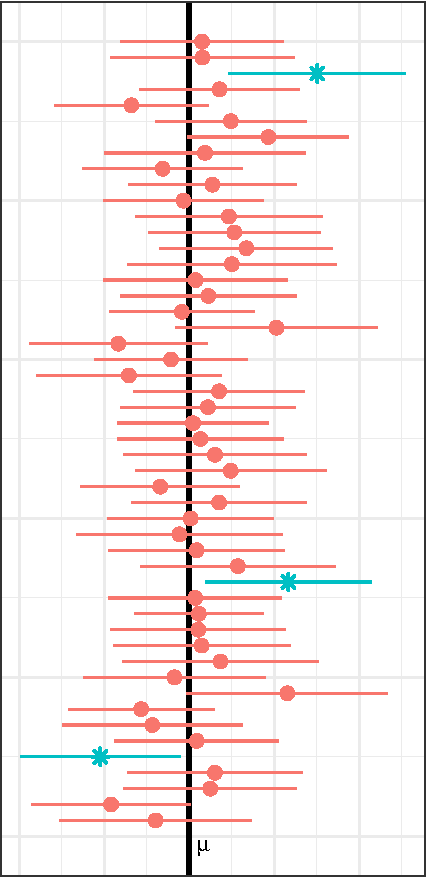
\includegraphics{02-basics-stat-infer_files/figure-pdf/fig-fifty-cis-1.pdf}

}

\caption{\label{fig-fifty-cis}Fifty \(95\%\) CIs for a population mean
\(\mu.\) After a sample is taken, the computed interval estimate either
contains \(\mu\) or does not (asterisks identify intervals that do not
include \(\mu\)). When drawing such a large number of \(95\%\) CIs, we
would anticipate that approximately \(5\%\) (ca. 2 or 3) would fail to
cover the true parameter \(\mu.\)}

\end{figure}%

\section{Hypothesis testing}\label{sec-hypothesis-testing}

Section~\ref{sec-point-estimation} and
Section~\ref{sec-confidence-intervals} reviewed how to estimate a
parameter by a single number (point estimate) or range of plausible
values (confidence interval), respectively. Next, we discuss methods for
determining which of two contradictory claims, or hypotheses, about a
parameter is correct.

\begin{definition}[Null and
alternative]\protect\hypertarget{def-null-alt-hypothesis}{}\label{def-null-alt-hypothesis}

The null hypothesis, denoted by \(H_0,\) is a claim we initially assume
to be true by default. The alternative hypothesis, denoted by \(H_a,\)
is an assertion contradictory to \(H_0.\)

\end{definition}

Typically, we shall consider a hypothesis test concerning a parameter
\(\theta \in \Theta,\) i.e., taking values in a parameter space
\(\Theta.\) The statistical hypotheses are contradictory in that \(H_0\)
and \(H_a\) divide \(\Theta\) into two disjoint sets. For example, for a
statistical inference regarding the \emph{equality} of a parameter
\(\theta\) with a fixed quantity \(\theta_0,\) the null and alternative
hypotheses will usually take one of the following forms in
Table~\ref{tbl-htest-null-alt-forms}.

\begin{longtable}[]{@{}
  >{\raggedright\arraybackslash}p{(\columnwidth - 4\tabcolsep) * \real{0.3333}}
  >{\raggedright\arraybackslash}p{(\columnwidth - 4\tabcolsep) * \real{0.3333}}
  >{\raggedright\arraybackslash}p{(\columnwidth - 4\tabcolsep) * \real{0.3333}}@{}}
\caption{Typical null hypothesis and corresponding alternative
hypothesis.}\label{tbl-htest-null-alt-forms}\tabularnewline
\toprule\noalign{}
\begin{minipage}[b]{\linewidth}\raggedright
Null hypothesis
\end{minipage} & \begin{minipage}[b]{\linewidth}\raggedright
Alternative hypothesis
\end{minipage} & \begin{minipage}[b]{\linewidth}\raggedright
Test form
\end{minipage} \\
\midrule\noalign{}
\endfirsthead
\toprule\noalign{}
\begin{minipage}[b]{\linewidth}\raggedright
Null hypothesis
\end{minipage} & \begin{minipage}[b]{\linewidth}\raggedright
Alternative hypothesis
\end{minipage} & \begin{minipage}[b]{\linewidth}\raggedright
Test form
\end{minipage} \\
\midrule\noalign{}
\endhead
\bottomrule\noalign{}
\endlastfoot
\(H_0 : \theta = \theta_0\) & \(H_a : \theta \neq \theta_0\) & two-sided
test \\
\(H_0 : \theta \leq \theta_0\) & \(H_a : \theta > \theta_0\) & one-sided
test \\
\(H_0 : \theta \geq \theta_0\) & \(H_a : \theta < \theta_0\) & one-sided
test \\
\end{longtable}

These hypothesis pairs are associated with either a one-sided or
two-sided test; what this means will become apparent in the sequel. The
value \(\theta_0,\) called the null value, separates the alternative
from the null.

\begin{definition}[Hypothesis
test]\protect\hypertarget{def-hypothesis-test}{}\label{def-hypothesis-test}

A hypothesis test asks if the available data provides sufficient
evidence to reject \(H_0.\) If the observations disagree with \(H_0,\)
we reject the null hypothesis. If the sample evidence does not strongly
contradict \(H_0,\) then we continue to believe \(H_0.\) The two
possible conclusions of a hypothesis test are: \emph{reject \(H_0\)} or
\emph{fail to reject \(H_0\)}.

\end{definition}

\begin{tcolorbox}[enhanced jigsaw, toprule=.15mm, leftrule=.75mm, colframe=quarto-callout-important-color-frame, arc=.35mm, rightrule=.15mm, bottomrule=.15mm, coltitle=black, title=\textcolor{quarto-callout-important-color}{\faExclamation}\hspace{0.5em}{``Fail to reject'' versus ``accept''}, breakable, colbacktitle=quarto-callout-important-color!10!white, bottomtitle=1mm, left=2mm, toptitle=1mm, titlerule=0mm, opacityback=0, opacitybacktitle=0.6, colback=white]

We comment that \emph{fail to reject \(H_0\)} is sometimes phrased as
\emph{retain \(H_0\)} or (perhaps less accurately) \emph{accept
\(H_0\)}.

Why not just \emph{accept} the null and move on with our lives?

Well, if I search the Highlands for the Scottish wildcat (endangered)
and fail to find any, does that prove they do not exist?

\end{tcolorbox}

A procedure for carrying out a hypothesis test is based on specifying
two additional items: a test statistic and a corresponding rejection
region. A test statistic \(T\) is a function of the sample data (like an
estimator). The decision to reject or fail to reject \(H_0\) will
involve computing the test statistic. The rejection region \(R\) is the
collection of values of the test statistic for which \(H_0\) is to be
rejected in favour of the alternative, e.g., \[
R = \left\{ x : T(x) > c \right\}\,,
\] where \(c\) is referred to as a critical value. If a given sample
falls in the rejection region, we reject \(H_0.\) If \(X \in R\) (e.g.,
the calculated test statistic exceeds some critical value), we reject
\(H_0.\) The alternative is that \(X \not\in R\) and we fail to reject
the null in this case.

Two types of errors can be made when carrying out a hypothesis test. The
basis for choosing a rejection region involves considering these errors.

\begin{definition}[Error
types]\protect\hypertarget{def-error-types}{}\label{def-error-types}

A type I error occurs if \(H_0\) is rejected when \(H_0\) is actually
true. A type II error is made if we fail to reject \(H_0\) when \(H_0\)
is actually false.

\end{definition}

If a test's maximal type I error is fixed at an acceptably small value,
then the type II error decreases as the sample size increases. In
particular, a conclusion is reached in a hypothesis test by selecting a
significance level \(\alpha\) for the test linked to the maximal type I
error rate. Typically, \(\alpha = 0.10,\) \(0.05,\) \(0.01,\) or
\(0.001\) is selected for the significance level.

\begin{definition}[\(P\)-value]\protect\hypertarget{def-P-value}{}\label{def-P-value}

A \(P\)-value is the probability, calculated assuming \(H_0\) is true,
of obtaining a value of the test statistic at least as contradictory to
\(H_0\) as the value calculated from the sample data.

\end{definition}

Smaller \(P\)-values indicate stronger evidence against \(H_0\) in favor
of \(H_a.\) If \(P \leq \alpha\) then we reject \(H_0\) at significance
level \(\alpha.\) If \(P \geq \alpha\) we fail to reject \(H_0\) at
significance level \(\alpha.\)

\begin{tcolorbox}[enhanced jigsaw, toprule=.15mm, leftrule=.75mm, colframe=quarto-callout-warning-color-frame, arc=.35mm, rightrule=.15mm, bottomrule=.15mm, coltitle=black, title=\textcolor{quarto-callout-warning-color}{\faExclamationTriangle}\hspace{0.5em}{What a \(P\)-value isn't\ldots{}}, breakable, colbacktitle=quarto-callout-warning-color!10!white, bottomtitle=1mm, left=2mm, toptitle=1mm, titlerule=0mm, opacityback=0, opacitybacktitle=0.6, colback=white]

The \(P\)-value is a probability calculated assuming that \(H_0\) is
true. However, the \(P\)-value is \textbf{not} the probability that:

\begin{enumerate}
\def\labelenumi{\arabic{enumi}.}
\tightlist
\item
  \(H_0\) is TRUE,
\item
  \(H_0\) is FALSE, or
\item
  a wrong conclusion is reached.
\end{enumerate}

\end{tcolorbox}

\begin{proposition}[]\protect\hypertarget{prp-signifiance-type1}{}\label{prp-signifiance-type1}

The hypothesis test procedure that \[
\begin{cases} 
\text{rejects}\; H_0 & \text{if}\; P \leq \alpha,\\
\text{fails to reject}\; H_0 & \text{otherwise},
\end{cases}
\] has \(P(\text{type I error}) = \alpha.\)

\end{proposition}

\begin{example}[]\protect\hypertarget{exm-htest-setup}{}\label{exm-htest-setup}

Churchill claims that he will receive half the votes for the House of
Commons seat for the constituency of Dundee.\footnote{Sir Winston
  Churchill was Member of Parliament for Dundee from 1908--1922
  {[}\url{https://www.wikiwand.com/en/Winston_Churchill}{]}.} If we do
not believe Churchill's claim and are doubtful of his popularity, we
would seek to test an alternative hypothesis. How should we write down
our research hypotheses?

If we let \(p\) be the fraction of the population voting for Churchill,
then we have the null hypothesis, \[
 H_0 : p = 0.5 \,,
\] and the alternative hypothesis (we believe Churchill is less popular
than he claims), \[
 H_a : p < 0.5 \,.
\] Support for the alternative hypothesis is obtained by showing a lack
of support for its converse hypothesis (the null hypothesis).

\end{example}

\begin{example}[]\protect\hypertarget{exm-htest-alpha}{}\label{exm-htest-alpha}

Suppose that \(m = 15\) voters are selected from Dundee and \(X,\) the
number favouring Churchill, is recorded. Based on observing \(X,\) we
construct a rejection region \(R = \{x : x \leq k \}.\) If \(k\) is
small compared to \(m,\) then the rejection region would provide strong
evidence to reject \(H_0.\) How should one choose the rejection region?

Assume now that \(m = 15\) voters are polled and that we select
\(k = 2\) to have a rejection region \(R = \{ x \leq 2 \}.\) For this
choice of \(k,\) the rejection region \(R\) provides strong support to
reject \(H_0.\) Assuming the null hypothesis is true, we expect
approximately half of the \(15\) voters (ca. 7) to vote for Churchill.
Observing \(x = 0,\) \(x = 1\) or \(x = 2\) (the values that would place
us in the rejection region) would provide strong evidence \emph{against}
\(H_0.\)

We can calculate the probability of a type I error. From the definition
of type I error, \[
 \begin{aligned}
 \alpha &= P(\text{type I error})\\
  &= P(\text{rejecting } H_0 \text{ when } H_0 \text{ is true})\\
  &= P(X \in R \text{ when } H_0 \text{ is true})\\
  &= P(X \leq 2 \text{ when } p = 0.5) \,.
 \end{aligned}
\] Since \(X \sim \mathsf{Binom}(15, 0.50),\) we calculate that
\(\alpha = 0.00369.\) Thus, for this particular choice of rejection
region \(R,\) the risk of concluding that Churchill will lose if, in
fact, he is the winner is tiny.

For this rejection region, how good is the test at protecting us from
type II errors, i.e., concluding that Churchill is the winner if, in
fact, he will lose? Suppose that Churchill receives \(25%
\) of the votes (\(p=0.25\)). The probability of type II error \(\beta\)
is, \[
  \begin{aligned}
  \beta &= P(\text{type II error})\\
  &= P(\text{fail to reject } H_0 \text{ when } H_0 \text{ false})\\
  &= P(X \not\in R \text{ when } H_0 \text{ false})\\
  &= P(X > 2 \text{ when } p = 0.3)\,.
 \end{aligned}
\] For \(X \sim \mathsf{Binom}(15, 0.25),\) we calculate
\(\beta = 0.764.\) If we use \(R = \{ x \leq 2\},\) then our test will
lead us to conclude that Churchill is the winner with a probability of
\(0.764\) even if \(p\) is as low as \(0.25\)!

If we repeat these calculations for \(R^* = \{x \leq 5\},\) we find
\(\alpha = 0.151\) versus \(\beta = 0.148,\) even if \(p\) is as low as
\(0.25,\) which is a much better balance between type I and type II
errors.

\end{example}

\begin{tcolorbox}[enhanced jigsaw, toprule=.15mm, leftrule=.75mm, colframe=quarto-callout-warning-color-frame, arc=.35mm, rightrule=.15mm, bottomrule=.15mm, coltitle=black, title=\textcolor{quarto-callout-warning-color}{\faExclamationTriangle}\hspace{0.5em}{What if the sample size is close to the population size?}, breakable, colbacktitle=quarto-callout-warning-color!10!white, bottomtitle=1mm, left=2mm, toptitle=1mm, titlerule=0mm, opacityback=0, opacitybacktitle=0.6, colback=white]

In Example~\ref{exm-htest-alpha}, \(X\) is a binomial random variable
because it can be modelled as \(m\) independent Bernoulli trails each
with probability \(p\) of success (i.e., votes for Churchill) as long as
the sample size \(m\) is much smaller than the population of Dundee. If
we had the means to canvas nearly the whole population, what goes wrong
conceptually?

\end{tcolorbox}

\begin{figure}

\centering{

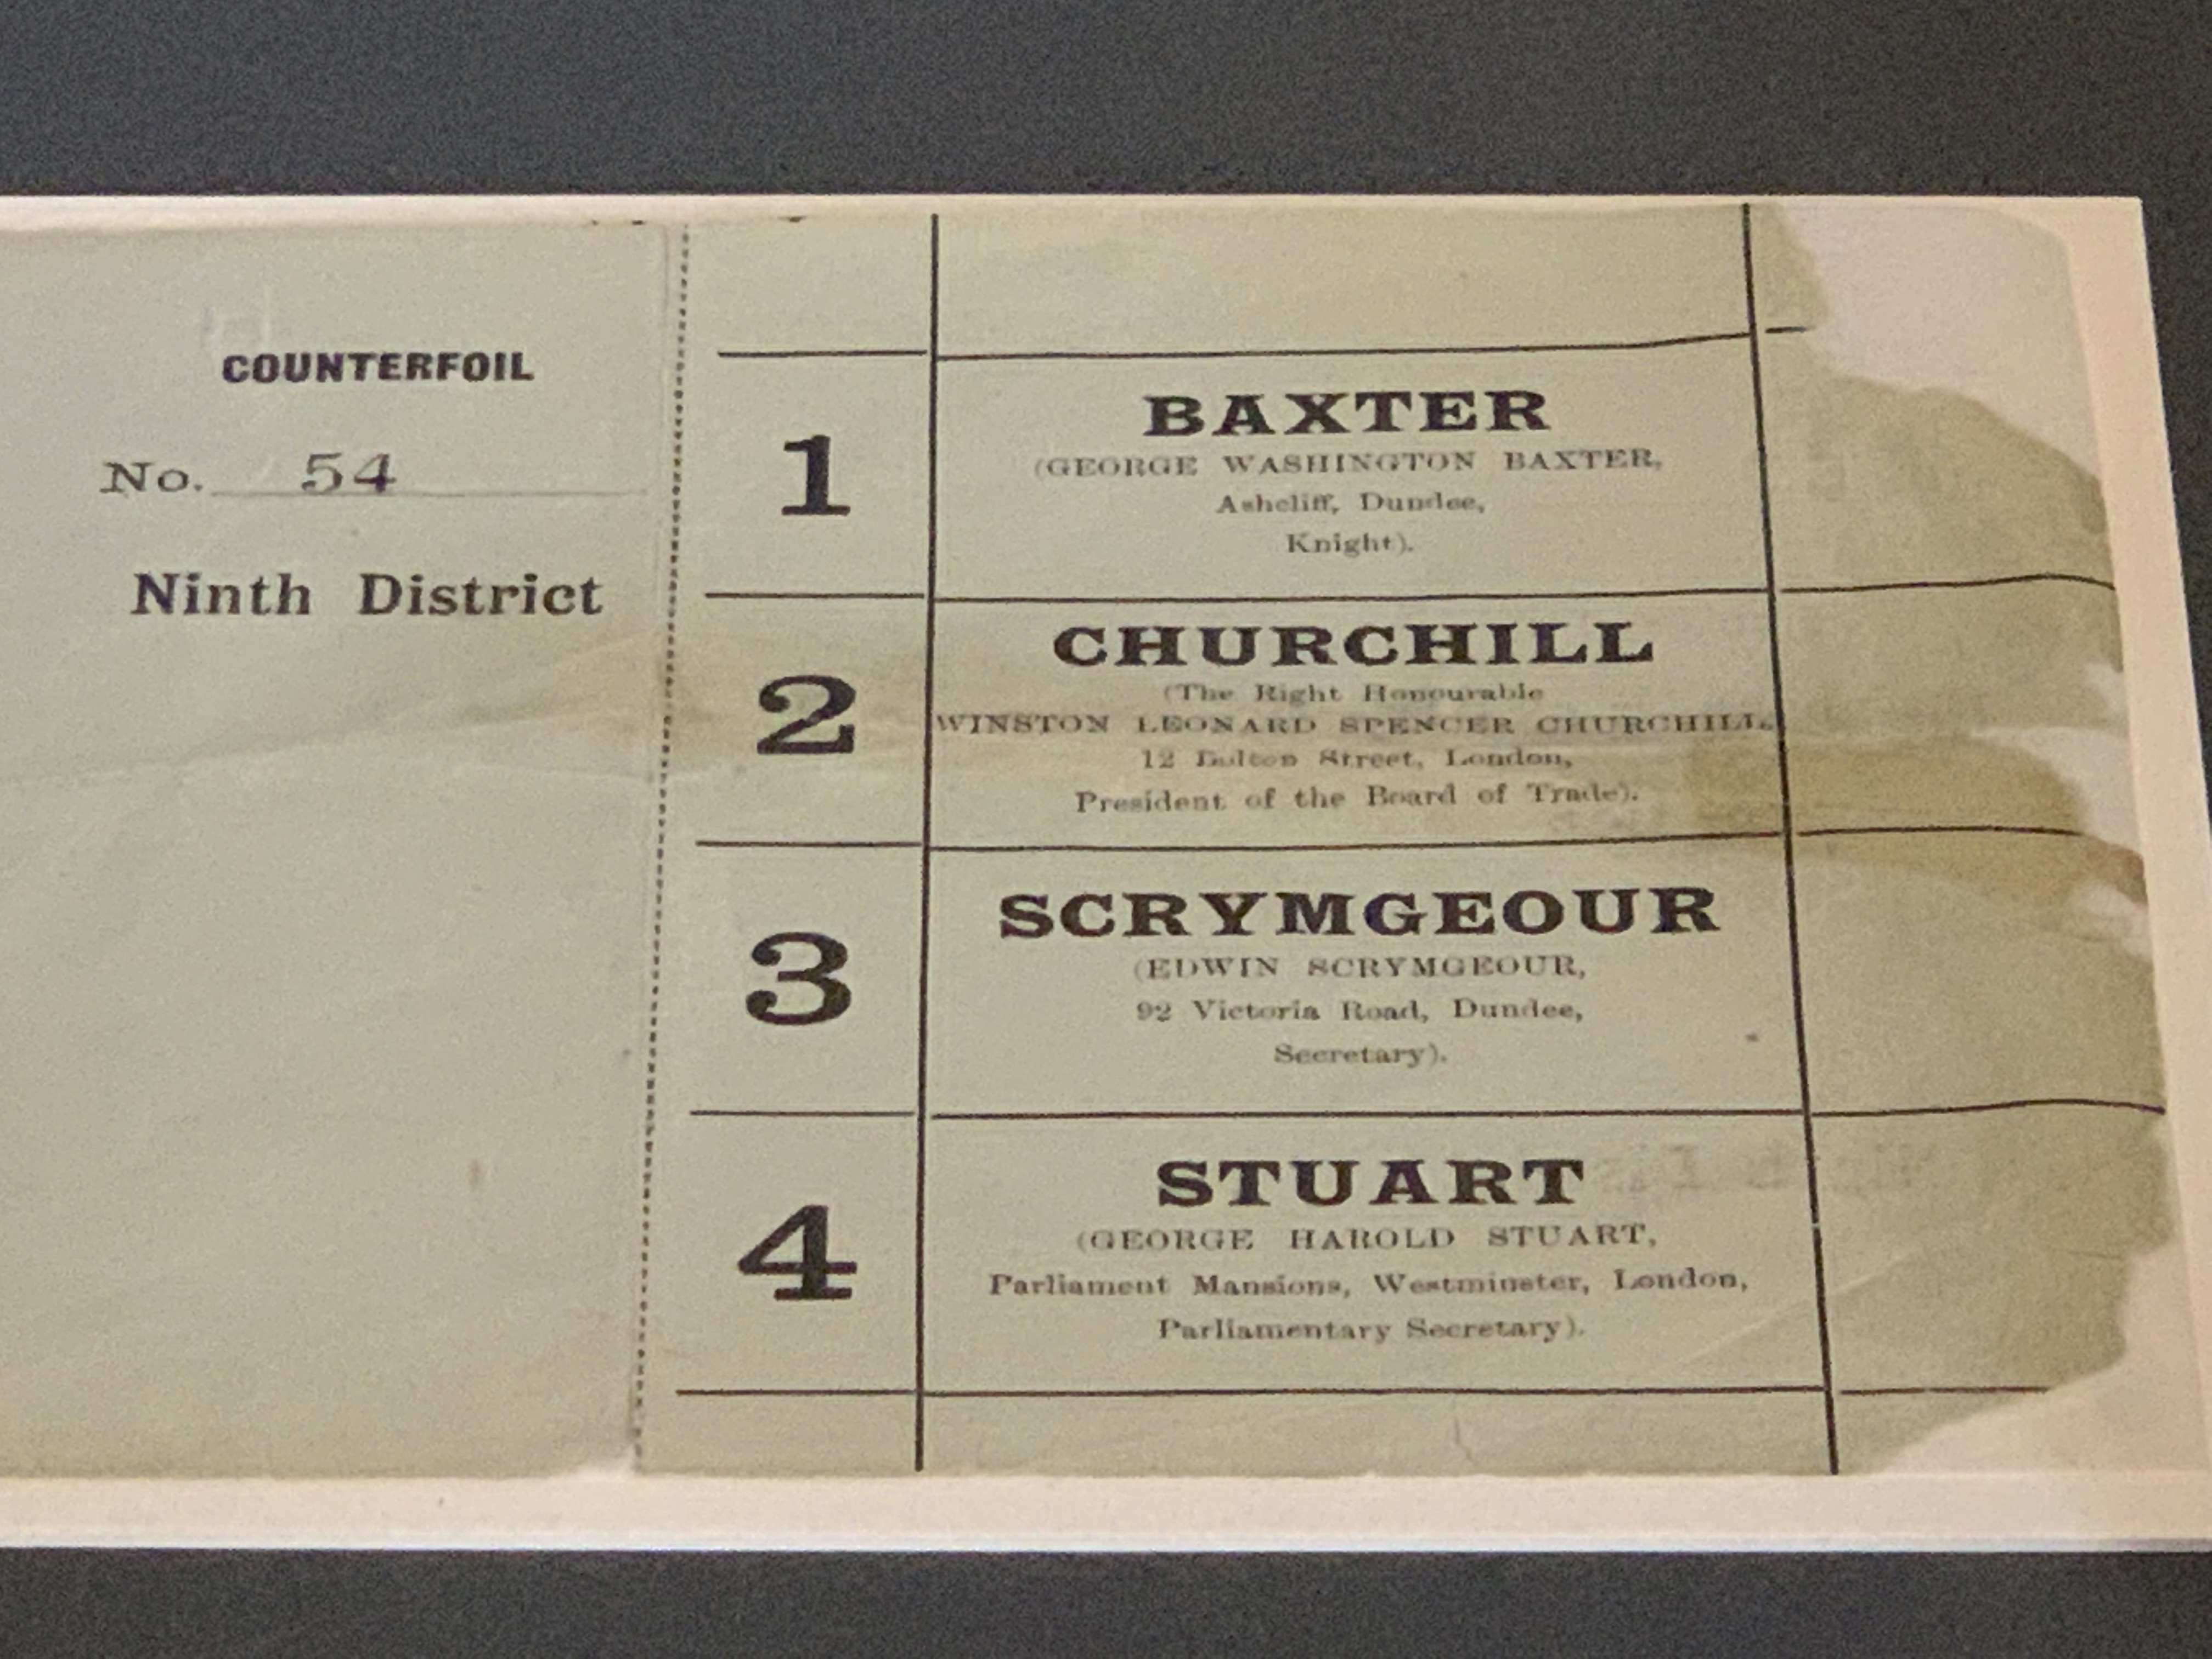
\includegraphics{assets/images/churchill_ballot.jpg}

}

\caption{\label{fig-churchill-ballot}Ballot listing Churchill from the
collection of the McManus, Dundee. When you take a break from studying,
go and see if you can find it! For more information on visiting the
McManus visit \url{https://www.mcmanus.co.uk/}.}

\end{figure}%

\begin{tcolorbox}[enhanced jigsaw, toprule=.15mm, leftrule=.75mm, colframe=quarto-callout-important-color-frame, arc=.35mm, rightrule=.15mm, bottomrule=.15mm, coltitle=black, title=\textcolor{quarto-callout-important-color}{\faExclamation}\hspace{0.5em}{Elements of a statistical test}, breakable, colbacktitle=quarto-callout-important-color!10!white, bottomtitle=1mm, left=2mm, toptitle=1mm, titlerule=0mm, opacityback=0, opacitybacktitle=0.6, colback=white]

A statistical test is based on a null hypothesis (\(H_0\)) and an
alternative hypothesis (\(H_a\)).

An appropriate test statistic \(T\) is computed. Then either:

\begin{itemize}
\tightlist
\item
  \(T\) is compared to a rejection region (based on significance level
  \(\alpha\))
\end{itemize}

OR

\begin{itemize}
\tightlist
\item
  \(P\)-value (based on \(T\)) is compare to the significance level
  \(\alpha.\)
\end{itemize}

\end{tcolorbox}

\chapter{Single sample inferences}\label{sec-inference-single-sample}

In a few situations, we can derive the sampling distribution for the
statistic of interest and use this as the basis for constructing
confidence intervals and hypothesis tests. Presently we estimate
population means \(\mu\) in Section~\ref{sec-estimating-means},
population proportions \(p\) in
Section~\ref{sec-estimating-proportions}, and population variances
\(\sigma^2\) in Section~\ref{sec-estimating-variances} in some special
cases.

\section{Estimating means}\label{sec-estimating-means}

If the parameter of interest is the population mean \(\theta = \mu\),
then what can be said about the distribution of the sample mean
estimator \(\widehat{\theta} = \overline{X}\) in
Equation~\ref{eq-sample-mean}? We will consider three cases,

\begin{enumerate}
\def\labelenumi{\arabic{enumi}.}
\tightlist
\item
  \hyperref[sec-mean-normal-var-known]{normal population with known
  \(\sigma^2\)},
\item
  \hyperref[sec-mean-large-sample]{any population with unknown
  \(\sigma^2\), when the sample size \(m\) is large}, and
\item
  \hyperref[sec-mean-normal-var-unknown]{normal population with unknown
  \(\sigma^2\), when the sample size \(m\) is small}.
\end{enumerate}

In each, the form of the confidence interval and hypothesis test
statistic for \(\mu\) can be derived using the approximate normality of
the sample mean.

In general, the confidence intervals for the mean based on normality
theory will have the form:
\begin{equation}\phantomsection\label{eq-ci-gen-form}{
 \text{point estimate}\; \mu \pm (\text{critical value}) \cdot (\text{precision of point estimate})\,, 
}\end{equation} where the reference distribution will be the standard
normal (for 1. and 2.) and the Student's \(\mathsf{t}\) distribution
(for 3.). The critical value corresponds to the value under the
reference distribution that yields the two-sided (symmetric) tail areas
summing to \(1-\alpha.\)

\subsection{Mean of a normal population with known
variance}\label{sec-mean-normal-var-known}

When sampling from a normal population with a known mean and variance,
the estimator for the sample mean is also normal with mean \(\mu\) and
variance \(\sigma^2/m\) where \(m\) is the sample size. Standardising,
\begin{equation}\phantomsection\label{eq-standardized-sample-mean}{
 \frac{\overline{X} - \mu}{ \sigma / \sqrt{m}} \quad \sim \mathsf{N}(0, 1)
}\end{equation} we see that \[
P\left(-z_{\alpha/2} <  \frac{\overline{X} - \mu}{ \sigma / \sqrt{m}} < z_{\alpha/2}\right) = 1 - \alpha\,.
\] Based on knowing the estimator's sampling distribution, we state the
following CI.

\begin{definition}[Confidence interval for mean of normal
population]\protect\hypertarget{def-ci-norm-known-var}{}\label{def-ci-norm-known-var}

A \(100(1-\alpha)\%\) confidence interval for the mean \(\mu\) of a
normal population when the value of \(\sigma^2\) is known is given by
\begin{equation}\phantomsection\label{eq-ci-norm-known-var}{
 \left(\overline{x} - z_{\alpha/2} \cdot \frac{\sigma}{\sqrt{m}}\,, 
        \overline{x} + z_{\alpha/2} \cdot \frac{\sigma}{\sqrt{m}} \right)\,, 
}\end{equation} or
\(\overline{x} \pm z_{\alpha/2} \cdot \sigma / \sqrt{m}\), where \(m\)
is the sample size.

\end{definition}

The CI for the mean Equation~\ref{eq-ci-norm-known-var} can be expressed
(cf. Equation~\ref{eq-ci-gen-form}) as \[
 \text{point estimate}\; \mu \pm 
 (z \;\text{critical value}) \cdot (\text{standard error of mean})\,.
\] The \(z\) critical value is related to the tail areas under the
standard normal curve; we need to find the \(z\)-score having a
cumulative probability equal to \(1-\alpha\) according to Definition
@ref(def:confidence-interval-gen).

\begin{example}[]\protect\hypertarget{exm-ci-norm-known-var}{}\label{exm-ci-norm-known-var}

Consider \(400\) samples from a normal population with a known standard
deviation \(\sigma = 17000\) with mean \(\overline{x} = 20992\) as
depicted in Figure~\ref{fig-ci-norm-known-var-code}. How do we construct
a \(95\%\) confidence interval for \(\mu\)?

\begin{figure}

\centering{

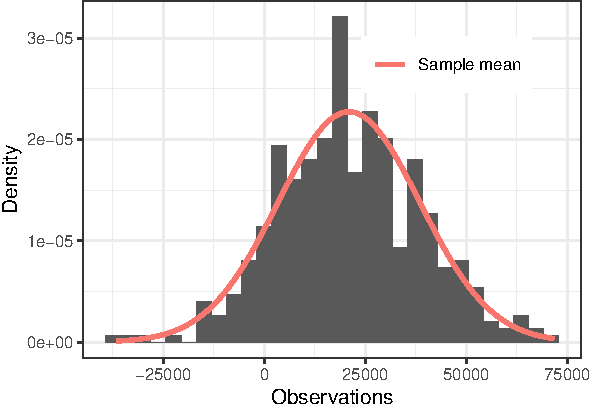
\includegraphics{03-infer-single-sample_files/figure-pdf/fig-ci-norm-known-var-code-1.pdf}

}

\caption{\label{fig-ci-norm-known-var-code}\(400\) samples from a normal
population with known variance \(\sigma = 17000\) together with the
corresponding (normal) sampling distribution for the observed mean.}

\end{figure}%

For \(\alpha = 0.05\), the critical value \(z_{0.025} = 1.96\); this
value can be found by looking in a table of critical \(z\) values or
using the \texttt{R} code \texttt{qnorm(1-.05/2)}. From
Definition~\ref{def-ci-norm-known-var}, \[
\begin{aligned}
\left(\overline{x} - z_{\alpha/2} \frac{\sigma}{\sqrt{m}}\,, \overline{x} + z_{\alpha/2} \frac{\sigma}{\sqrt{m}} \right) 
&= \left(20992 - 1.96 \frac{17000}{\sqrt{400}}\,, 20992 + 1.96 \frac{17000}{\sqrt{400}} \right) \\
&= \left(19326 \,, 22658\right)\,.
\end{aligned}
\]

The data above was generated with a true population parameter
\(\mu = 21500\), and the CI contains the parameter value (incidentally).

\end{example}

As noted in Equation~\ref{eq-ci-gen-form} and
Equation~\ref{eq-ci-norm-known-var}, the width of a CI is related to the
estimator's precision. The confidence level (or reliability) is
inversely related to this precision. When the population is normal and
the variance is known, determining the sample size necessary to achieve
a desired confidence level and precision is an appealing strategy. A
general formula for the sample size \(m^*\) necessary to achieve an
interval width \(w\) is obtained at confidence level \(\alpha\) by
equating \[w = 2z_{\alpha/2} \cdot \sigma /\sqrt{m^*}\] and then solving
for \(m^*.\)

\begin{proposition}[]\protect\hypertarget{prp-ci-select-n-fixed-w-alpha}{}\label{prp-ci-select-n-fixed-w-alpha}

The sample size \(m\) required to achieve a CI for \(\mu\) with width
\(w\) at level \(\alpha\) is given by, \[
m^* = \left( 2 z_{\alpha/2} \cdot \frac{\sigma}{w} \right)^2 \,.
\]

\end{proposition}

From Proposition~\ref{prp-ci-select-n-fixed-w-alpha}, we see that the
smaller the desired \(w\), the larger \(m^*\) must be (and subsequently,
the more effort that must be allocated to data collection).

\begin{example}[]\protect\hypertarget{exm-ci-norm-known-var-find-n}{}\label{exm-ci-norm-known-var-find-n}

In Example~\ref{exm-ci-norm-known-var} we identified a \(95\%\)
confidence interval for a normal population with known variance. The
range (width) of that interval was \(22658 - 19326 = 3332.\) How much
would \(m\) need to increase to halve the interval width?

Using Proposition~\ref{prp-ci-select-n-fixed-w-alpha}, \[
m = \left( 2 \cdot 1.96 \cdot \frac{17000}{1666} \right)^2 = (40)^2 = 1600\,.
\] Thus, we find that for the same level \(\alpha = 0.05\), we would
need to quadruple our original sample size to halve the interval.

\end{example}

\begin{tcolorbox}[enhanced jigsaw, toprule=.15mm, leftrule=.75mm, colframe=quarto-callout-warning-color-frame, arc=.35mm, rightrule=.15mm, bottomrule=.15mm, coltitle=black, title=\textcolor{quarto-callout-warning-color}{\faExclamationTriangle}\hspace{0.5em}{You heard it here first\ldots{}}, breakable, colbacktitle=quarto-callout-warning-color!10!white, bottomtitle=1mm, left=2mm, toptitle=1mm, titlerule=0mm, opacityback=0, opacitybacktitle=0.6, colback=white]

As Example~\ref{exm-ci-norm-known-var-find-n} shows, it is expensive to
reduce uncertainty!

\end{tcolorbox}

Suppose now that we would like to consider a hypothesis test for the
population mean, such as \(H_0 : \mu = \mu_0.\) Starting from
Equation~\ref{eq-standardized-sample-mean} and assuming that the null
hypothesis is true, we find \[
Z = \frac{\overline{X} - \mu_0}{\sigma / \sqrt{m}}\,.
\] The statistic \(Z\) measures the distance (measured in units of
\(\mathop{\mathrm{sd}}[\overline{X}]\)) between \(\overline{X}\) and its
expected value under the null hypothesis. We will use the statistic
\(Z\) to determine if there is substantial evidence against \(H_0\),
i.e.~if the distance is too far in a direction consistent with \(H_a.\)

\begin{proposition}[]\protect\hypertarget{prp-htest-norm-known-var}{}\label{prp-htest-norm-known-var}

Assume that we sample \(X_1, \dots, X_m\) from a normal population with
mean \(\mu\) and known variance \(\sigma^2.\)

Consider \(H_0 : \mu = \mu_0.\) The test statistic is
\begin{equation}\phantomsection\label{eq-htest-norm-known-var-T}{
 Z = \frac{\overline{X} - \mu_0}{\sigma / \sqrt{m}}\,.
}\end{equation}

For a hypothesis test at level \(\alpha\), we use the following
procedure:

If \(H_a : \mu > \mu_0\), then \(P = 1 - \Phi(z)\), i.e., upper-tail
\(R = \{z > z_{\alpha}\}.\)

If \(H_a : \mu < \mu_0\), then \(P = \Phi(z)\), i.e., lower-tail
\(R = \{z < - z_{\alpha}\}.\)

If \(H_a : \mu \neq \mu_0\), then \(P = 2(1-\Phi(|z|))\), i.e.,
two-tailed \(R = \{|z| > z_{\alpha/2}\}.\)

\end{proposition}

We recall that \(\Phi(z)\) is the area in the lower tail of the standard
normal density, i.e., to the \emph{left} of the calculated value of
\(z.\) Thus \(1 - \Phi(z)\) is the area in the upper-tail, and
\(2(1 - \Phi(|z|))\) is twice the area captured in the upper-tail by
\(|z|\), i.e.~the sum of the area in the tails corresponding to
\(\pm z.\) If \(P < \alpha\), then we reject \(H_0\) at level \(\alpha\)
as the data provides sufficient evidence at the \(\alpha\) level against
the null hypothesis.

\begin{example}[]\protect\hypertarget{exm-htest-norm-known-var-two-tail}{}\label{exm-htest-norm-known-var-two-tail}

Let's return to the data in Example~\ref{exm-ci-norm-known-var}, where
we sample from a normal population with a known standard deviation
\(\sigma = 17000.\) Suppose that someone claims the true mean is
\(\mu_0 = 20000.\) Does our sample mean \(\overline{x} = 20992\) based
on \(m = 400\) samples provide evidence to contradict this claim at the
\(\alpha = 0.05\) level?

The first thing to record is our parameter of interest: \(\mu\), the
true population mean. The null hypothesis, which we assume to be true,
is a statement about the value of \(\mu\), \[
 H_0 : \mu = 20000\,,
\] and the alternative hypothesis is \[
 H_a : \mu \neq 20000\,,
\] since we are concerned with a deviation in either direction from
\(\mu_0 = 20000.\)

Since the population is normal with known variance, we compute the test
statistic: \[
 z = \frac{\overline{x} - \mu_0}{\sigma / \sqrt{m}} = \frac{20992 - 20000}{17000 / \sqrt{400}} = 1.167\,.
\] That is, the observed sample mean \(\overline{x}\) is slightly more
than \(1\) standard deviation than what we expect under \(H_0.\)
Consulting Proposition~\ref{prp-htest-norm-known-var}, we see that a
two-tailed test is indicated for this particular \(H_a\) (i.e.,
containing ``\(\neq\)''). The \(P\)-value is the area, \[
P = 2(1 - \Phi(1.167)) = 2 (0.1216052) = 0.2432.
\] Thus, since \(P = 0.2432 > 0.05 = \alpha\), we fail to reject \(H_0\)
at the level \(0.05.\) The data does not support the claim that the true
population mean differs from the value \(20000\) at the \(0.05\) level.

\end{example}

\begin{tcolorbox}[enhanced jigsaw, toprule=.15mm, leftrule=.75mm, colframe=quarto-callout-tip-color-frame, arc=.35mm, rightrule=.15mm, bottomrule=.15mm, coltitle=black, title=\textcolor{quarto-callout-tip-color}{\faLightbulb}\hspace{0.5em}{Recall}, breakable, colbacktitle=quarto-callout-tip-color!10!white, bottomtitle=1mm, left=2mm, toptitle=1mm, titlerule=0mm, opacityback=0, opacitybacktitle=0.6, colback=white]

Note \(\Phi(z) = P(Z \leq z)\) is found by calling \texttt{pnorm(z)} in
\texttt{R} or by looking up the value in a \(Z\) table.

\end{tcolorbox}

\subsection{Mean of a population with unknown variance
(large-sample)}\label{sec-mean-large-sample}

Consider samples \(X_1, \dots, X_m\) from a population with mean \(\mu\)
and variance \(\sigma^2.\) Provided that \(m\) is large enough, the
Central Limit Theorem implies that the estimator for the sample mean
\(\overline{X}\) in Equation~\ref{eq-sample-mean} has
\emph{approximately} a normal distribution. Then \[
P \left( - z_{\alpha/2} < \frac{\overline{X} - \mu}{\sigma/\sqrt{m}} < z_{\alpha/2} \right) \approx 1 - \alpha\,,
\] since the transformed variable has approximately a standard normal
distribution. Thus, computing a point estimate based on a large \(m\) of
samples yields a CI for the population parameter \(\mu\) at an
\emph{approximate} confidence level \(\alpha.\) However, it is often the
case that the variance is unknown. When \(m\) is large, replacing the
population variance \(\sigma^2\) by the sample variance \(S^2\) in
Equation~\ref{eq-sample-var} will not typically introduce too much
additional variability.

\begin{proposition}[]\protect\hypertarget{prp-ci-large-sample}{}\label{prp-ci-large-sample}

For a large sample size \(m\), an approximate \(100(1-\alpha)\%\)
confidence interval for the mean \(\mu\) of any population when the
variance is unknown is given by
\begin{equation}\phantomsection\label{eq-ci-large-sample}{
 \left(\overline{x} - z_{\alpha/2} \cdot \frac{s}{\sqrt{m}} \,, 
        \overline{x} + z_{\alpha/2} \cdot \frac{s}{\sqrt{m}} \right)\,,  
}\end{equation} or \(\overline{x} \pm z_{\alpha/2} \cdot s / \sqrt{m}.\)

\end{proposition}

The CI for the mean Equation~\ref{eq-ci-large-sample} applies regardless
of the shape of the population distribution so long as the number of
samples is large. A rule of thumb is that \(m > 40\) is sufficient. In
words, the CI Equation~\ref{eq-ci-large-sample} can be expressed (cf.
Equation~\ref{eq-ci-gen-form}) as \[
 \text{point estimate}\; \mu \pm 
 (z \;\text{critical value}) \cdot (\text{estimated standard error of mean})\,.
\] Typically, a large-sample CI for a general parameter \(\theta\) holds
that is similar to Equation~\ref{eq-ci-large-sample} for any estimator
\(\widehat{\theta}\) that satisfies: (1) approximately normal in
distribution, (2) approximately unbiased, and (3) an expression for the
standard error is available.

To conduct a large-sample hypothesis test regarding the population mean
\(\mu\), we consider the test statistic \[
 Z = \frac{\overline{X} - \mu_0}{S / \sqrt{m}}
\] under the null hypothesis, i.e., we replace the population standard
deviation \(\sigma\) with the sample standard deviation \(S.\) When the
number of samples \(m\) is large (say \(m > 40\)), then \(Z\) will be
approximately normal. Substituting this test statistic \(Z\) for
Equation~\ref{eq-htest-norm-known-var-T}, we follow
Proposition~\ref{prp-htest-norm-known-var} to determine how to calculate
the \(P\)-value.

\begin{tcolorbox}[enhanced jigsaw, toprule=.15mm, leftrule=.75mm, colframe=quarto-callout-tip-color-frame, arc=.35mm, rightrule=.15mm, bottomrule=.15mm, coltitle=black, title=\textcolor{quarto-callout-tip-color}{\faLightbulb}\hspace{0.5em}{Rule of thumb}, breakable, colbacktitle=quarto-callout-tip-color!10!white, bottomtitle=1mm, left=2mm, toptitle=1mm, titlerule=0mm, opacityback=0, opacitybacktitle=0.6, colback=white]

For estimating means, we consider a sample size of \(m > 40\) to be
large.

However, `large' depends on the context: for example, the level of
support for the evidence that you are seeking. For \(m > 20\), the
interval estimate \[\text{point estimate } \pm 2\mathop{\mathrm{sd}}\]
has \(95\%\) coverage and is surprisingly robust, i.e.~applies to a wide
variety of population distributions including the normal. However, this
rule of thumb won't apply if you want to consider some different level,
say \(80\%\) (\citeproc{ref-vanBelle:2008rt}{Belle 2008, sec. 1}).

\end{tcolorbox}

\begin{example}[]\protect\hypertarget{exm-mean-large-sample-infer}{}\label{exm-mean-large-sample-infer}

Let's consider the \textbf{Iris Data} from Note~\ref{nte-iris} and use
the \texttt{infer} package to make inferences. In particular, consider
whether there is evidence at the \(0.05\) level to support the statement
that the true mean petal length of Iris flowers exceeds \(3.5\) cm.

Recall that the \textbf{Iris Data} contains \(m= 150\) measurements of
petal length across three species of Iris flowers and that the true
variance is unknown. We are interested in testing the null hypothesis,
\[H_0 : \mu \leq 3.5\,,\] against the alternative,
\[H_a : \mu > 3.5\,,\] i.e., a one-sided test.

We first compute the observed statistic (sample mean) \(\widehat{\mu}.\)
We use the \texttt{infer} package to construct a null distribution
\emph{computationally} for the response variable (petal length). We
specify that the hypothesis test is for the parameter based on a point
estimate and that we are testing for equality with the value
\(\mu_0 = 3.5.\) The null distribution is generated by computing 1000
bootstrap replications of the sample mean, i.e., the sample mean is
generated 1000 times by drawing 150 values at random with replacement
from the original corpus of \(m=150\) samples. (Note that we obtain the
null distribution computationally, so we do not need to standardise to
\(Z.\))

\begin{Shaded}
\begin{Highlighting}[]
\NormalTok{mu\_hat }\OtherTok{\textless{}{-}} \FunctionTok{mean}\NormalTok{(iris}\SpecialCharTok{$}\NormalTok{Petal.Length) }

\NormalTok{null\_dist }\OtherTok{\textless{}{-}}\NormalTok{ iris }\SpecialCharTok{|\textgreater{}}
 \FunctionTok{specify}\NormalTok{(}\AttributeTok{response =}\NormalTok{ Petal.Length) }\SpecialCharTok{|\textgreater{}}
 \FunctionTok{hypothesise}\NormalTok{(}\AttributeTok{null =} \StringTok{"point"}\NormalTok{, }\AttributeTok{mu =} \FloatTok{3.5}\NormalTok{) }\SpecialCharTok{|\textgreater{}}
 \FunctionTok{generate}\NormalTok{(}\AttributeTok{reps =} \DecValTok{1000}\NormalTok{, }\AttributeTok{type =} \StringTok{"bootstrap"}\NormalTok{) }\SpecialCharTok{|\textgreater{}}
 \FunctionTok{calculate}\NormalTok{(}\AttributeTok{stat =} \StringTok{"mean"}\NormalTok{)}

\NormalTok{null\_dist }\SpecialCharTok{|\textgreater{}}
 \FunctionTok{visualise}\NormalTok{() }\SpecialCharTok{+}
 \FunctionTok{shade\_p\_value}\NormalTok{(}\AttributeTok{obs\_stat =}\NormalTok{ mu\_hat, }\AttributeTok{direction =} \StringTok{"greater"}\NormalTok{)}
\end{Highlighting}
\end{Shaded}

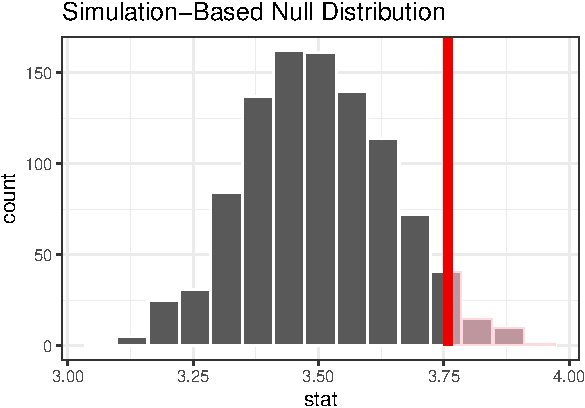
\includegraphics{03-infer-single-sample_files/figure-pdf/unnamed-chunk-2-1.pdf}

The bootstrapped null distribution is plotted using the
\texttt{visualise} command, and the regions of the null distribution
that are as extreme (or more extreme) than the observed statistic
\(\widehat{\mu}\) can be highlighted using the \texttt{shade\_p\_value}
command.

\begin{Shaded}
\begin{Highlighting}[]
\NormalTok{p\_val }\OtherTok{\textless{}{-}}\NormalTok{ null\_dist }\SpecialCharTok{|\textgreater{}}
 \FunctionTok{get\_p\_value}\NormalTok{(}\AttributeTok{obs\_stat =}\NormalTok{ mu\_hat, }\AttributeTok{direction =} \StringTok{"greater"}\NormalTok{)}
\NormalTok{p\_val}
\end{Highlighting}
\end{Shaded}

\begin{verbatim}
# A tibble: 1 x 1
  p_value
    <dbl>
1   0.042
\end{verbatim}

The test yields a \(P\)-value of \(P = 0.042.\) This values is quite
small; if \(\mu \leq 3.5\), then the probability of obtaining the sample
mean value \(\widehat{\mu} = 3.758\) is only 0.042! Thus, the data
provide sufficient evidence at the 0.05 level against the hypothesis
that the true mean petal length is at most 3.5 cm.

\end{example}

\subsection{Mean of a normal population with unknown
variance}\label{sec-mean-normal-var-unknown}

In Section~\ref{sec-mean-normal-var-known}, we considered samples
\(X_1, \dots, X_m\) from a normal population with a known \(\mu\) and
\(\sigma^2.\) In contrast, here, we consider samples from a normal
population and assume the population parameters \(\mu\) and \(\sigma^2\)
are unknown. If the number of samples is large, the discussion in
Section~\ref{sec-mean-large-sample} indicates that the rv
\[Z = (\overline{X} - \mu) \sqrt{m} / S \] has approximately a standard
normal distribution. However, if \(m\) is not sufficiently large then
the transformed variable will be more spread out than a standard normal
distribution.

\begin{theorem}[]\protect\hypertarget{thm-sample-mean-t-dist}{}\label{thm-sample-mean-t-dist}

For the sample mean \(\overline{X}\) based on \(m\) samples from a
normal distribution with mean \(\mu\), the rv
\begin{equation}\phantomsection\label{eq-t-statistic-mean}{
 T = \frac{\overline{X} - \mu}{S/\sqrt{m}}  \quad \sim \mathsf{t}(m-1)\,,
}\end{equation} that is, \(T\) has Student's \(\mathsf{t}\) distribution
with \(\nu = m-1\) df.

\end{theorem}

This leads us to consider a CI for the population parameter \(\mu\)
based on critical values of the \(\mathsf{t}\) distribution.

\begin{proposition}[]\protect\hypertarget{prp-ci-norm-unknown-var}{}\label{prp-ci-norm-unknown-var}

A \(100(1-\alpha)\%\) confidence interval for the mean \(\mu\) of a
normal population, when \(\sigma^2\) is unknown, is given by
\begin{equation}\phantomsection\label{eq-ci-norm-unknown-var}{
 \left(\overline{x} - t_{\alpha/2, m-1} \cdot \frac{s}{\sqrt{m}}\,, 
        \overline{x} + t_{\alpha/2, m-1} \cdot \frac{s}{\sqrt{m}} \right)\,, 
}\end{equation} or
\(\overline{x} \pm t_{\alpha/2, m-1} \cdot s/ \sqrt{m}.\) Here
\(\overline{x}\) and \(s\) are the sample mean and sample standard
deviation, respectively.

\end{proposition}

\begin{example}[]\protect\hypertarget{exm-ci-norm-unknown-var}{}\label{exm-ci-norm-unknown-var}

Let us return to the height of \(31\) felled black cherry trees from the
\textbf{Cherry Tree Data} in Note~\ref{nte-tree}. Give a \(99\%\) CI for
the population mean \(\mu.\)

For \(m = 31\), the critical value of the reference distribution is
\[t_{0.005, 30} \approx 2.7499\,,\] which can looked up in a table of
critical values for \(\mathsf{t}(\nu = 30)\) or found using the
\texttt{R} command \texttt{qt(1-0.01/2,\ df\ =\ 31-1)}. The sample mean
\(\overline{x} = 76\) (computed in Example~\ref{exm-estimators}) is
combined with the sample standard deviation, \[
\begin{aligned}
 s &= \sqrt{\frac{1}{m-1} \sum_{i=1}^m (x_i - \overline{x})^2}\\ 
   &= \sqrt{\frac{1}{30} \left((63-76)^2 + \cdots + (87 - 76)^2\right)}\\
   &= 6.372\,,
 \end{aligned}
\] to form the interval estimate \[
\begin{aligned}
& \left(\overline{x} - t_{\alpha/2, m-1}  \cdot \frac{s}{\sqrt{m}}\,, 
        \overline{x} + t_{\alpha/2, m-1} \cdot \frac{s}{\sqrt{m}} \right) \\
        &\qquad = \left(76 - 2.750 \cdot \frac{6.372}{\sqrt{31}} \,, 76 + 2.750 \cdot \frac{6.372}{\sqrt{31}} \right)\\
        &\qquad = \left(72.85\,, 79.15\right)\,.
\end{aligned}
\] For comparison, the critical value \(t_{.01/2, \nu}\) for
\(\nu = 14, \dots, 40\) can be recalled with the following command.

\begin{Shaded}
\begin{Highlighting}[]
\FunctionTok{qt}\NormalTok{(}\DecValTok{1}\FloatTok{{-}0.01}\SpecialCharTok{/}\DecValTok{2}\NormalTok{, }\AttributeTok{df =} \FunctionTok{seq}\NormalTok{(}\DecValTok{14}\NormalTok{,}\DecValTok{40}\NormalTok{))}
\end{Highlighting}
\end{Shaded}

\begin{verbatim}
 [1] 2.976843 2.946713 2.920782 2.898231 2.878440 2.860935 2.845340 2.831360 2.818756
[10] 2.807336 2.796940 2.787436 2.778715 2.770683 2.763262 2.756386 2.749996 2.744042
[19] 2.738481 2.733277 2.728394 2.723806 2.719485 2.715409 2.711558 2.707913 2.704459
\end{verbatim}

Note that these critical values can deviate significantly from the
corresponding \(z_{0.01/2} = 2.575829.\) In particular, if we had
erroneously used the large sample estimate
Equation~\ref{eq-ci-large-sample}, then we would have obtained a
\(99\%\) CI \((73.05\,, 78.95)\) which might give us a false sense of
security as it is narrower.

\end{example}

In contrast to Proposition~\ref{prp-ci-select-n-fixed-w-alpha}, it is
difficult to select the sample size \(m\) to control the width of the
\(\mathsf{t}\)-based CI as the width involves the unknown (before the
sample is acquired) \(s\) and because \(m\) also enters through
\(t_{\alpha/2, m-1}.\) A one-sample \(\mathsf{t}\) test based on
Equation~\ref{eq-t-statistic-mean} can be used to test a hypothesis
about the population mean when the population is normal and \(\sigma^2\)
is unknown.

\begin{proposition}[]\protect\hypertarget{prp-htest-mean-normal-var-unknown}{}\label{prp-htest-mean-normal-var-unknown}

Assume that we sample \(X_1, \dots, X_m\) from a normal population with
mean \(\mu\) and unknown variance \(\sigma^2.\)

Consider \(H_0 : \mu = \mu_0.\) The test statistic is \[
 T = \frac{\overline{X} - \mu_0}{S / \sqrt{m}} \,.
\]

For a hypothesis test at level \(\alpha\), we use the following
procedure:

If \(H_a : \mu > \mu_0\), then \(P\)-value is the area under
\(\mathsf{t}(m-1)\) to the right of \(t.\)

If \(H_a : \mu < \mu_0\), then \(P\)-value is the area under
\(\mathsf{t}(m-1)\) to the left of \(t.\)

If \(H_a : \mu \neq \mu_0\), then \(P\)-value is twice the area under
\(\mathsf{t}(m-1)\) to the right of \(|t|.\)

\end{proposition}

\begin{example}[]\protect\hypertarget{exm-htest-ttest}{}\label{exm-htest-ttest}

Let's consider the \textbf{Cherry Tree Data} in Note~\ref{nte-tree}. The
average timber volume is given in Table~\ref{tbl-cherry-data-vol}. The
distribution for this data is approximately normal. We might ask if the
data provide compelling evidence, say at level 0.05, for concluding that
the true average timber volume exceeds 21.3 cubic feet.\footnote{How
  much wood is that? About a sixth of a cord. A full cord of chopped
  firewood in the US is \(124\) cu ft; about enough to keep you warm
  through a New England winter (according to my mother-in-law).}

\begin{table}

\caption{\label{tbl-cherry-data-vol}Observations of \(m = 31\) felled
black cherry trees.}

\centering{

\centering
\begin{tabular}[t]{>{\raggedright\arraybackslash}p{150mm}}
\toprule
Volume [cu ft]\\
\midrule
\cellcolor{gray!10}{10.2, 10.3, 10.3, 15.6, 16.4, 18.2, 18.8, 19.1, 19.7, 19.9, 21.0, 21.3, 21.4, 22.2, 22.6, 24.2, 24.9, 25.7, 27.4, 31.7, 33.8, 34.5, 36.3, 38.3, 42.6, 51.0, 51.5, 55.4, 55.7, 58.3, 77.0}\\
\bottomrule
\end{tabular}

}

\end{table}%

Let's carry out a significance test for the true average volume of
timber \(\mu\) at level \(\alpha = 0.05.\) We assume the null hypothesis
\[
 H_0 : \mu = 21.3\,.
\] An appropriate alternative hypothesis is \[
 H_a : \mu > 21.3\,,
\] that is, we will adopt the stance that the true average exceeds
\(\mu_0 = 21.3\) only if the null is rejected.

From our \(m = 31\) samples, we find that \(\overline{x} = 30.17\) and
that \(s = 16.44.\) The computed value of the one-sample
\(\mathsf{t}\)-statistic is given by \[
\begin{aligned}
 t &= \frac{\overline{x} - \mu_0}{s / \sqrt{m}}\\
 &= \frac{30.17 - 21.3}{16.44 / \sqrt{31}}\\
 & = 3\,.
 \end{aligned}
\] The test is based on \(\nu = 31-1\) df, and \(P = 0.002663.\) This is
the upper-tail area, i.e., the area to the right of \(t\) in
Figure~\ref{fig-exm-htest-ttest-plot}. Since \(P \ll \alpha\), we reject
the null hypothesis that the population mean is \(21.3.\) The data
provide sufficient evidence that the population mean differs from
\(21.3.\)

\begin{figure}

\centering{

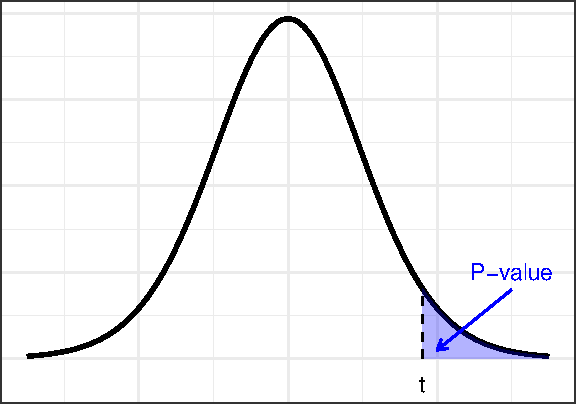
\includegraphics{03-infer-single-sample_files/figure-pdf/fig-exm-htest-ttest-plot-1.pdf}

}

\caption{\label{fig-exm-htest-ttest-plot}For this test, the reference
distribution is \(\mathsf{t}(\nu = 30)\) (\textbf{not} a Normal
distribution) and the \(P\)-value is the upper-tail area, i.e., to the
right of the computed statistic \(t.\)}

\end{figure}%

\end{example}

\begin{tcolorbox}[enhanced jigsaw, toprule=.15mm, leftrule=.75mm, colframe=quarto-callout-important-color-frame, arc=.35mm, rightrule=.15mm, bottomrule=.15mm, coltitle=black, title=\textcolor{quarto-callout-important-color}{\faExclamation}\hspace{0.5em}{Shapiro-Wilk normality test}, breakable, colbacktitle=quarto-callout-important-color!10!white, bottomtitle=1mm, left=2mm, toptitle=1mm, titlerule=0mm, opacityback=0, opacitybacktitle=0.6, colback=white]

We can assess the normality of the sample by examining the normal
quantile-quantile plot as in Example~\ref{exm-estimators}. For the data
in Example~\ref{exm-htest-ttest} recall that this is done using the
following \texttt{R} code.

\begin{Shaded}
\begin{Highlighting}[]
\NormalTok{trees }\SpecialCharTok{|\textgreater{}} \FunctionTok{ggplot}\NormalTok{(}\FunctionTok{aes}\NormalTok{(}\AttributeTok{sample =}\NormalTok{ Volume)) }\SpecialCharTok{+} \FunctionTok{stat\_qq}\NormalTok{() }\SpecialCharTok{+} \FunctionTok{stat\_qq\_line}\NormalTok{()}
\end{Highlighting}
\end{Shaded}

\begin{figure}[H]

\centering{

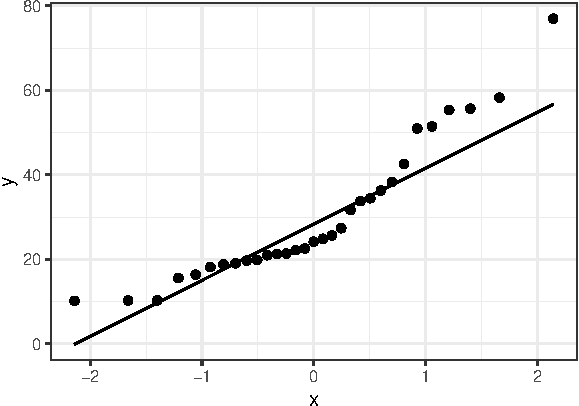
\includegraphics{03-infer-single-sample_files/figure-pdf/fig-qq-plot-cherry-vol-1.pdf}

}

\caption{\label{fig-qq-plot-cherry-vol}Normal quantile-quantile plot for
the \texttt{Volume} variable (feature) in the Cherry Tree Data.}

\end{figure}%

The data deviates quite a bit in the centre and in the tails of the
distribution, indicating that there might be a moderate departure from
normality.

It is also possible to test the null hypothesis that the data is
consistent with a normal distribution versus the alternative that the
data is not normal. This is called a Shapiro-Wilk normality test.

\begin{Shaded}
\begin{Highlighting}[]
\FunctionTok{shapiro.test}\NormalTok{(trees}\SpecialCharTok{$}\NormalTok{Height)}
\end{Highlighting}
\end{Shaded}

\begin{verbatim}

    Shapiro-Wilk normality test

data:  trees$Height
W = 0.96545, p-value = 0.4034
\end{verbatim}

At level \(0.05\), the Shapiro-Wilk test yields a \(P\)-value
\(P = 0.4034 > 0.05\), and therefore we fail to reject the null
hypothesis. We cannot exclude that the data is drawn from a normal
population. This ``prove'' the data is drawn from a normal distribution,
but it does tell us that for this particular example, an inference based
on a normal distribution instead of a \(\mathsf{t}\) distribution will
probably be reasonable. It is always good to view the QQ plot as well
--- sometimes if the number of samples is very large then the
Shapiro-Wilk test will reject the null for trivial deviations from
normality.

\end{tcolorbox}

\section{Estimating proportions}\label{sec-estimating-proportions}

Consider a population of size \(M\) in which each member either
satisfies a given property or does not (i.e.~a binary classification).
The proportion \(p \in (0,1)\) of the population satisfying the given
property is a parameter characterising the population we might be
interested in estimating. A sample of classified observations,
\(X_1, \dots, X_m \sim \mathsf{Bernoulli}(p)\,,\) from the population
contains a proportion,
\begin{equation}\phantomsection\label{eq-proportion-estimator}{
 \widehat{p} = \frac{1}{m} \sum_{i=1}^m X_i\,,
}\end{equation} satisfying the given property. The estimator
\(\widehat{p}\) varies with the sample, and for large \(m\), its
sampling distribution has the following properties:
\begin{equation}\phantomsection\label{eq-proportion-mean}{
\mu_{\widehat{p}} = \mathbf{E}[X_i] = p 
}\end{equation} and
\begin{equation}\phantomsection\label{eq-proportion-var}{
 \sigma_{\widehat{p}}^2 = \frac{\mathop{\mathrm{Var}}[X_i]}{m} = \frac{p(1-p)}{m}\,,
}\end{equation} provided that \(m\) is small relative to \(M.\)
Moreover, by invoking the Central Limit Theorem, we have the
distribution of \(\widehat{p}\) is approximately normal for sufficiently
large \(m\) as Equation~\ref{eq-proportion-estimator} is a sample mean.
Indeed, this normal approximation works well for moderately large \(m\)
as long as \(p\) is not too close to zero or one; a rule of thumb is
that \(mp > 5\) and \(m(1-p) > 5.\)

\begin{tcolorbox}[enhanced jigsaw, toprule=.15mm, leftrule=.75mm, colframe=quarto-callout-tip-color-frame, arc=.35mm, rightrule=.15mm, bottomrule=.15mm, coltitle=black, title=\textcolor{quarto-callout-tip-color}{\faLightbulb}\hspace{0.5em}{Rule of thumb}, breakable, colbacktitle=quarto-callout-tip-color!10!white, bottomtitle=1mm, left=2mm, toptitle=1mm, titlerule=0mm, opacityback=0, opacitybacktitle=0.6, colback=white]

For estimating proportions, a rule of thumb is \(m \leq 0.05 M.\)

Note that if \(m\) is large relative to \(M\) (\(m > 0.05 M\)) then the
variance Equation~\ref{eq-proportion-var} must be adjusted by a factor
(related to the hypergeometric distribution): \[
 \sigma_{\widehat{p}}^2 = \frac{p(1-p)}{m} \frac{M-m}{M-1}\,,
\] where for fixed \(m\) the factor converges to \(1\) as
\(M\to \infty.\)

\end{tcolorbox}

\begin{proposition}[]\protect\hypertarget{prp-ci-proportion}{}\label{prp-ci-proportion}

For large samples \(n\), a \(100(1-\alpha)\%\) confidence interval for
the parameter \(p\) is given by
\begin{equation}\phantomsection\label{eq-proportion-mean-ci}{
 \widehat{p} \pm z_{\alpha/2} \sqrt{\frac{\widehat{p} (1-\widehat{p})}{m}}\,.
}\end{equation}

\end{proposition}

This follows from Proposition~\ref{prp-ci-large-sample} by observing
that Equation~\ref{eq-proportion-estimator} is a sample mean and
replacing the standard error \(\sigma_{\widehat{p}}\) from
Equation~\ref{eq-proportion-var} by the estimated standard error, \[
 \widehat{\mathsf{se}}(\widehat{p}) = \sqrt{\frac{\widehat{p} (1-\widehat{p})}{m}}\,;
\] recall the \(s\) in Equation~\ref{eq-ci-large-sample}) is the sample
variance for the \emph{population} and \(s / \sqrt{m} = \mathsf{se}\) is
the standard error of the point estimator.

\begin{proposition}[]\protect\hypertarget{prp-htest-proportion}{}\label{prp-htest-proportion}

Let \(X\) be the count of members with a given property based on a
sample of size \(m\) from a population where a proportion \(p\) shares
the property. Then \(\widehat{p} = X / m\) is an estimator of \(p.\)
Assume \(m p_0 \geq 10\) and \(m (1-p_0) \geq 10.\)

Consider \(H_0 : p = p_0.\) The test statistic is \[
 Z = \frac{\widehat{p} - p_0}{\sqrt{p_0 (1-p_0) / m}} \,.
\]

For a hypothesis test at level \(\alpha\), we use the following
procedure:

If \(H_a : p > p_0\), then \(P\)-value is the area under
\(\mathsf{N}(0,1)\) to the right of \(z.\)

If \(H_a : p < p_0\), then \(P\)-value is the area under
\(\mathsf{N}(0,1)\) to the left of \(z.\)

If \(H_a : p \neq p_0\), then \(P\)-value is twice the area under
\(\mathsf{N}(0,1)\) to the right of \(|z|.\)

\end{proposition}

\begin{example}[]\protect\hypertarget{exm-est-prop-hypothesis-test}{}\label{exm-est-prop-hypothesis-test}

Let us revisit Example~\ref{exm-htest-setup}, where we considered
Churchill's claim that he would receive half the votes for the House of
Commons seat for the constituency of Dundee. We are sceptical that he is
as popular as he says. Suppose 116 out of 263 Dundonians polled claimed
they intended to vote for Churchill. Can it be concluded at a
significance level of \(0.10\) that more than half of all eligible
Dundonains will vote for Churchill?

The parameter of interest is \(p\), the proportion of votes for
Churchill. The null hypothesis is \[H_0 : p = 0.5\,,\] and the
alternative hypothesis is, \[H_a : p < 0.5\,.\] The test is oneside
(i.e.~\(H_a : p < 0.5\)) since we are interested in testing support for
``more than half''. Since \(263(0.5) = 131.5 > 10\), we satisfy the
assumptions stated in Proposition~\ref{prp-htest-proportion}.

Based on the sample, \(\widehat{p} = 116 / 263 = 0.4411.\) The test
statistic value is \[
\begin{aligned}
 z &= \frac{\widehat{p} - p_0}{\sqrt{p_0 (1-p_0) / m}} \\
 &= \frac{0.4411 - 0.5}{\sqrt{0.5 (1-0.5) / 263}}\\
 &= -1.91  \,.
\end{aligned}
\] The \(P\)-value for this lower-tailed \(z\) test is
\(P = \Phi(-1.91) = 0.028.\) Since \(P < 0.10 = \alpha\), we reject the
null hypothesis at the \(0.1\) level. The evidence for concluding that
the true proportion is different from \(p_0 = 0.5\) at the \(0.10\)
level is compelling.\footnote{Churchill took ca. \(44\%\) of the vote in
  the 1908 by-election to become MP for Dundee
  {[}\url{https://www.wikiwand.com/en/1908_Dundee_by-election}{]}.}

\end{example}

\section{Estimating variances}\label{sec-estimating-variances}

Next, we consider estimates of the population variance (and standard
deviation) when the population is assumed to have a normal distribution.
In this case, the sample variance \(S^2\) in
Equation~\ref{eq-sample-var} provides the basis for inferences. Consider
iid samples \(X_1, \dots, X_m \sim \mathsf{N}(\mu, \sigma^2).\) We
provide the following theorem without proof.

\begin{theorem}[]\protect\hypertarget{thm-samp-var-chisq}{}\label{thm-samp-var-chisq}

For the sample variance \(S^2\) based on \(m\) samples from a normal
distribution with variance \(\sigma^2\), the rv \[
V = \frac{(m-1)S^2}{\sigma^2} = \frac{\sum_i(X_i - \overline{X})^2}{\sigma^2} \qquad \sim \chi^2_{m-1}\,,
\] that is, \(V\) has a \(\chi^2\) distribution with \(\nu = m-1\) df.

\end{theorem}

Based on Theorem~\ref{thm-samp-var-chisq}, \[
P\left(\chi^2_{1-\alpha/2, m-1} < \frac{(m-1)S^2}{\sigma^2} < \chi^2_{\alpha/2, m-1} \right) = 1 - \alpha \,,
\] i.e., the area captured between the right and left tail critical
\(\chi^2\) values is \(1-\alpha.\) The expression above can be further
manipulated to obtain an interval for the unknown parameter
\(\sigma^2\): \[
P\left(\frac{(m-1) s^2}{\chi^2_{\alpha/2, m-1}} < \sigma^2 < \frac{(m-1) s^2}{\chi^2_{1-\alpha/2, m-1}} \right) = 1 - \alpha \,,
\] where we substitute the computed value of the point estimate \(s^2\)
for the estimator into the limits to give a CI for \(\sigma^2.\) If we
take square roots in the inequality above, we obtain a CI for the
population standard deviation \(\sigma.\)

\begin{proposition}[]\protect\hypertarget{prp-ci-variance}{}\label{prp-ci-variance}

A \(100(1-\alpha)\%\) confidence interval for the variance of a normal
population is \begin{equation}\phantomsection\label{eq-ci-variance}{
 \left( (m-1)s^2 / \chi^2_{\alpha/2, m-1} \,,  (m-1)s^2 / \chi^2_{1-\alpha/2, m-1} \right) \,.
}\end{equation} A \(100(1-\alpha)\%\) confidence interval for the
standard deviation \(\sigma\) of a normal population is given by taking
the square roots of the lower and upper limits in
Equation~\ref{eq-ci-variance}.

\end{proposition}

\begin{example}[]\protect\hypertarget{exm-eg-ci-variance}{}\label{exm-eg-ci-variance}

For the \textbf{Cherry Tree Data} in Table~\ref{tbl-cherry-data-vol}
concerning the timber volume of \(31\) felled black cherry trees, give a
\(95%
\) CI for the variance.

We are interested in estimating the true variance \(\sigma^2\) of the
timber volume based on \(m=31\) samples. Recall that the mean of our
data is \(\overline{x} = 30.17\) cu ft and that the sample variance is
\(s^2 = 270.2\) using the estimator Equation~\ref{eq-sample-var}. The
critical values for the \(\chi^2_{.975, 30} = 16.7908\) and
\(\chi^2{.025, 30} = 46.9792\) can be found by checking a table of
critical values of the \(\chi^2(\nu=30)\) distribution or by using the
\texttt{R} code \texttt{qchisq(1-0.05/2,\ df=30,\ lower.tail\ =\ FALSE)}
and \texttt{qchisq(0.05/2,\ df=df,\ lower.tail\ =\ FALSE)},
respectively, see Figure~\ref{fig-exm-htest-chisq-plot} below.

\begin{figure}

\centering{

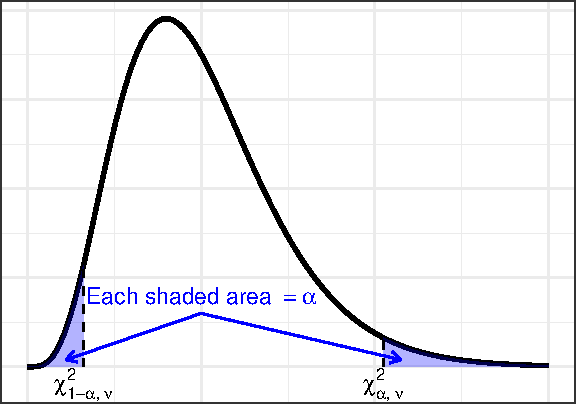
\includegraphics{03-infer-single-sample_files/figure-pdf/fig-exm-htest-chisq-plot-1.pdf}

}

\caption{\label{fig-exm-htest-chisq-plot}As the \(\chi^2\) distribution
is not symmetric, the upper and lower critical values will not be the
same (the shaded areas are equal).}

\end{figure}%

Pulling everything together, a \(95\%\) CI for the population variance
is given by \[
\begin{aligned}
 & \left( (m-1)s^2 / \chi^2_{\alpha/2, m-1} \,,  (m-1)s^2 / \chi^2_{1-\alpha/2, m-1} \right) \\
 &\qquad = \left( (30) 270.2 / 46.9792 \,, (30) 270.2 / 16.7908  \right) \\
 &\qquad = \left(172.5\,, 482.8\right)\,.
 \end{aligned}
\] Note the position of the critical values---don't swap them around.

\end{example}

\begin{example}[]\protect\hypertarget{exm-eg-ci-variance-infer}{}\label{exm-eg-ci-variance-infer}

Let's Revisit Example~\ref{exm-eg-ci-variance}) and use the
\texttt{infer} package to construct a \(95\%\) confidence interval for
the true standard deviation of the timber volume of black cherry trees
based on the available measurements in the \textbf{Cherry Tree Data},
Table~\ref{tbl-cherry-data-vol}).

\begin{Shaded}
\begin{Highlighting}[]
\NormalTok{s }\OtherTok{\textless{}{-}} \FunctionTok{sd}\NormalTok{(trees}\SpecialCharTok{$}\NormalTok{Volume)}

\NormalTok{null\_dist }\OtherTok{\textless{}{-}}\NormalTok{ trees }\SpecialCharTok{|\textgreater{}}
 \FunctionTok{specify}\NormalTok{(}\AttributeTok{response =}\NormalTok{ Volume) }\SpecialCharTok{|\textgreater{}}
 \FunctionTok{generate}\NormalTok{(}\AttributeTok{reps =} \DecValTok{1000}\NormalTok{, }\AttributeTok{type =} \StringTok{"bootstrap"}\NormalTok{) }\SpecialCharTok{|\textgreater{}}
 \FunctionTok{calculate}\NormalTok{(}\AttributeTok{stat =} \StringTok{"sd"}\NormalTok{)}

\NormalTok{ci }\OtherTok{\textless{}{-}}\NormalTok{ null\_dist }\SpecialCharTok{|\textgreater{}}
 \FunctionTok{get\_confidence\_interval}\NormalTok{(}\AttributeTok{point\_estimate =}\NormalTok{ s, }\AttributeTok{level =} \FloatTok{0.95}\NormalTok{, }\AttributeTok{type =} \StringTok{"se"}\NormalTok{)}

\NormalTok{null\_dist }\SpecialCharTok{|\textgreater{}} 
 \FunctionTok{visualise}\NormalTok{() }\SpecialCharTok{+} \FunctionTok{shade\_ci}\NormalTok{(ci)}
\end{Highlighting}
\end{Shaded}

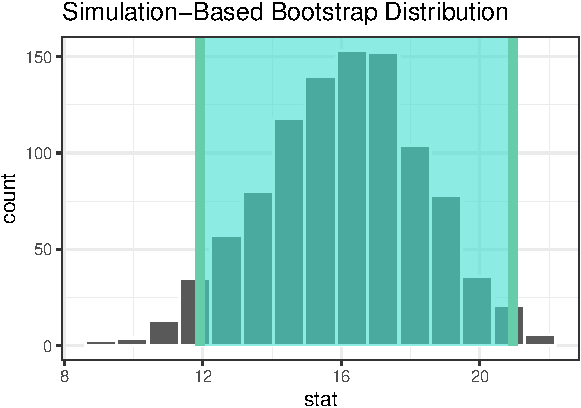
\includegraphics{03-infer-single-sample_files/figure-pdf/unnamed-chunk-10-1.pdf}

We plot the \(95\%\) confidence interval for the standard deviation
based on the computational null distribution obtained using 1000
bootstrap replications; note the interval estimate is in good agreement
with the values obtained in Example~\ref{exm-eg-ci-variance}.

\begin{Shaded}
\begin{Highlighting}[]
\NormalTok{ci}\SpecialCharTok{\^{}}\DecValTok{2}
\end{Highlighting}
\end{Shaded}

\begin{verbatim}
  lower_ci upper_ci
1 142.2009 438.9398
\end{verbatim}

Due to the computational nature, the bootstrapped interval estimate is
not precisely the same as the theoretical interval estimate and
rerunning the code will yield a slightly different interval.

\end{example}

\chapter{Two samples inferences}\label{sec-inference-two-samples}

We consider inferences---estimators, confidence intervals, and
hypothesis testing---for comparing means, proportions, and variances
based on two independent samples from different populations,
respectively, in Section~\ref{sec-compare-means},
Section~\ref{sec-compare-proportions},
Section~\ref{sec-compare-variances}. We also consider inferences when
the samples are not independent, so-called paired samples, in
Section~\ref{sec-compare-paired-samples}.

\section{Comparing means}\label{sec-compare-means}

Let us assume that we have two normal populations with iid samples \[
 X_1, \dots, X_m \sim \mathsf{N}(\mu_X, \sigma_X^2)
\] and \[
 Y_1, \dots, Y_n \sim \mathsf{N}(\mu_Y, \sigma_Y^2)
\] and, moreover, that the \(X\) and \(Y\) samples are independent of
one another. When comparing the means of two populations, the quantity
of interest is the difference: \(\mu_X - \mu_Y.\)

\begin{proposition}[]\protect\hypertarget{prp-qoi-diff-pop-means}{}\label{prp-qoi-diff-pop-means}

If we consider the sample means \(\overline{X}\) and \(\overline{Y},\)
then the mean of the variable \(\overline{X} - \overline{Y}\) is, \[
 \mu_{\overline{X} - \overline{Y}} 
= \mathbf{E}\left[ \overline{X} - \overline{Y} \right] = \mu_X - \mu_Y\,,
\] and the variance is, \[
 \sigma_{\overline{X} - \overline{Y}}^2
= \mathop{\mathrm{Var}}\left[ \overline{X} - \overline{Y} \right]
= \frac{\sigma_X^2}{m} + \frac{\sigma_Y^2}{n} \,.
\]

\end{proposition}

Proposition~\ref{prp-qoi-diff-pop-means} follows directly from the
definition of the sample mean in Equation~\ref{eq-sample-mean} and
properties of expectation and variance. If our parameter of interest is
\[
 \theta = \mu_1 - \mu_2\,,
\] then its estimator, \[
 \widehat{\theta} = \overline{X} - \overline{Y}\,,
\] is normally distributed with mean and variance given by
Proposition~\ref{prp-qoi-diff-pop-means}. If the sample sizes \(m\) and
\(n\) are large, then the estimator is approximately normally
distributed by the Central Limit Theorem regardless of the population.
We now discuss CIs and hypothesis tests for comparing population means
\(\theta = \mu_X - \mu_Y.\) We consider three cases when comparing
means:

\begin{enumerate}
\def\labelenumi{\arabic{enumi}.}
\tightlist
\item
  \hyperref[sec-compare-means-normpops-vars-known]{normal populations
  when the variances \(\sigma_X^2\) and \(\sigma_Y^2\) are known},
\item
  \hyperref[sec-compare-means-large-samples]{any populations with
  unknown variances \(\sigma_X^2\) and \(\sigma_Y^2,\) when the sample
  sizes \(m\) and \(n\) are large},
\item
  \hyperref[sec-compare-means-normpops-vars-unknown]{normal populations
  when the variances \(\sigma_X^2\) and \(\sigma_Y^2\) are unknown, when
  the sample sizes \(m\) and \(n\) are small},
\end{enumerate}

noting that the development primarily reflects that of
Section~\ref{sec-estimating-means}.

\subsection{Comparing means of normal populations when variances are
known}\label{sec-compare-means-normpops-vars-known}

When \(\sigma_X^2\) and \(\sigma_Y^2\) are known, standardizing
\(\overline{X} - \overline{Y}\) yields the standard normal variable:
\begin{equation}\phantomsection\label{eq-compare-means-standard-trans}{
 Z = \frac{\overline{X} - \overline{Y} - (\mu_X - \mu_Y)}{\sqrt{\frac{\sigma_X^2}{m} + \frac{\sigma_Y^2}{n}}}\quad \sim \mathsf{N}(0,1)\,.
}\end{equation}\\
Inferences proceed by treating the parameter of interest \(\theta\) as
in the single sample case using the test statistic
Equation~\ref{eq-compare-means-standard-trans}.

\begin{proposition}[]\protect\hypertarget{prp-ci-compare-means-normpops-vars-known}{}\label{prp-ci-compare-means-normpops-vars-known}

A \(100(1-\alpha)\%\) CI for the parameter \(\theta = \mu_X - \mu_Y\)
based on samples of size \(m\) from a normal population
\(\mathsf{N}(\mu_X, \sigma_X^2)\) and of size \(n\) from
\(\mathsf{N}(\mu_Y, \sigma_Y^2)\) with known variances, is given by \[
 (\overline{x} - \overline{y}) \pm z_{\alpha/2} 
 \cdot \sqrt{\frac{\sigma_X^2}{m} + \frac{\sigma_Y^2}{n}} \,.
\]

\end{proposition}

\begin{proposition}[]\protect\hypertarget{prp-htest-compare-means-normpops-vars-known}{}\label{prp-htest-compare-means-normpops-vars-known}

Assume that we sample iid
\(X_1, \dots, X_m \sim \mathsf{N}(\mu_X, \sigma_X^2)\) and iid
\(Y_1, \dots, Y_n \sim \mathsf{N}(\mu_Y, \sigma_Y^2)\) and that the
\(X\) and \(Y\) samples are independent.

Consider \(H_0 : \mu_X - \mu_Y = \theta_0.\) The test statistic is
\begin{equation}\phantomsection\label{eq-htest-compare-means-normpops-vars-known-statistic}{
 Z = \frac{\overline{X} - \overline{Y} - \theta_0}{\sqrt{\frac{\sigma_{X}^2}{m} + \frac{\sigma_{Y}^2}{n}}}\,.
}\end{equation}

For a hypothesis test at level \(\alpha,\) we use the following
procedure:

If \(H_a : \mu_X - \mu_Y > \theta_0,\) then \(P = 1 - \Phi(z),\) i.e.,
upper-tail \(R = \{z > z_{\alpha}\}.\)

If \(H_a : \mu_X - \mu_Y < \theta_0,\) then \(P = \Phi(z),\) i.e.,
lower-tail \(R = \{z < - z_{\alpha}\}.\)

If \(H_a : \mu_X - \mu_Y \neq \theta_0,\) then \(P = 2(1-\Phi(|z|)),\)
i.e., two-tailed \(R = \{|z| > z_{\alpha/2}\}.\)

\end{proposition}

\subsection{Comparing means when the sample sizes are
large}\label{sec-compare-means-large-samples}

When the samples are large, the assumptions about the normality of the
populations and knowledge of the variances \(\sigma_X^2\) and
\(\sigma_Y^2\) can be relaxed. For sufficiently large \(m\) and \(n,\)
the difference of the sample means, \(\overline{X} - \overline{Y},\) has
approximately a normal distribution for any underlying population
distributions by the Central Limit Theorem. Moreover, if \(m\) and \(n\)
are large enough, replacing the population variances with the sample
variances \(S_X^2\) and \(S_Y^2\) will not increase the variability of
the estimator or the test statistic too much.

\begin{proposition}[]\protect\hypertarget{prp-ci-compare-means-large-samples}{}\label{prp-ci-compare-means-large-samples}

For \(m\) and \(n\) sufficiently large, an approximate
\(100(1-\alpha)\%\) CI for \(\mu_X - \mu_Y\) for two samples from
populations with any underlying distribution is given by \[
 (\overline{x} - \overline{y}) \pm z_{\alpha/2} 
 \cdot \sqrt{\frac{s_{X}^2}{m} + \frac{s_{Y}^2}{n}}
\]

\end{proposition}

\begin{proposition}[]\protect\hypertarget{prp-htest-compare-means-large-samples}{}\label{prp-htest-compare-means-large-samples}

Under the same assumptions and procedures as in
Proposition~\ref{prp-htest-compare-means-normpops-vars-known}, a
large-sample, i.e., \(m > 40\) and \(n > 40,\) test statistic, \[
 Z = \frac{\overline{X} - \overline{Y} - \theta_0}{\sqrt{\frac{S_{X}^2}{m} + \frac{S_{Y}^2}{n}}}\,,
\] can be used in place of
Equation~\ref{eq-htest-compare-means-normpops-vars-known-statistic} for
hypothesis testing.

\end{proposition}

\subsection{Comparing means of normal populations when variances are
unknown and the sample size is
small}\label{sec-compare-means-normpops-vars-unknown}

If \(\sigma_X\) and \(\sigma_Y\) are unknown and either sample is small
(e.g., \(m < 30\) or \(n <30\)), but both populations are normally
distributed, then we can use Student's \(\mathsf{t}\) distribution to
make inferences. We provide the following theorem without proof.

\begin{theorem}[]\protect\hypertarget{thm-dist-t-compare-means-normpops}{}\label{thm-dist-t-compare-means-normpops}

When both population distributions are normal, the standardised variable
\[
T = \frac{\overline{X}-\overline{Y} - (\mu_X - \mu_Y)}{\sqrt{\frac{S_X^2}{m} + \frac{S_Y^2}{n}}} 
\quad \sim \mathsf{t}(\nu)\,,
\] where the df \(\nu\) is estimated from the data. Namely, \(\nu\) is
given by (round \(\nu\) down to the nearest integer):
\begin{equation}\phantomsection\label{eq-dist-t-compare-means-normpops-nu}{
 \nu = \frac{ \left( \frac{s_X^2}{m} + \frac{s_Y^2}{n} \right)^2}{\frac{(s_X^2 / m)^2}{m-1} + \frac{(s_Y^2/n)^2}{n-1}} 
 = \frac{ \left( s_{\overline{X}}^2 + s_{\overline{Y}}^2 \right)^2}{\frac{s_{\overline{X}}^4}{m-1} + \frac{s_{\overline{Y}}^4}{n-1}}\,,
}\end{equation} where \(s_X^2\) and \(s_Y^2\) are point estimators of
the sample variances; alternatively, we see that the formula
Equation~\ref{eq-dist-t-compare-means-normpops-nu} can also be written
in terms of the standard error of the sample means: \[
 s_{\overline{X}} = \frac{s_X}{\sqrt{m}} 
 \quad \text{and} \quad \qquad 
 s_{\overline{Y}} = \frac{s_Y}{\sqrt{n}} \,.
\]

\end{theorem}

The formula Equation~\ref{eq-dist-t-compare-means-normpops-nu} for the
data-driven choice of \(\nu\) calls for the computation of the standard
error of the sample means.

\begin{proposition}[]\protect\hypertarget{prp-ci-compare-means-normpops-vars-unknown}{}\label{prp-ci-compare-means-normpops-vars-unknown}

A \(100(1-\alpha)\%\) CI for \(\mu_X - \mu_Y\) for two samples of size
\(m\) and \(n\) from normal populations where the variances are unknown
is given by \[
 (\overline{x} - \overline{y}) \pm t_{\alpha/2, \nu} \sqrt{ \frac{s_X^2}{m} + \frac{s_Y^2}{n}}\,,
\] where we recall that \(t_{\alpha/2, \nu}\) is the \(\alpha/2\)
critical value of \(\mathsf{t}(\nu)\) with \(\nu\) given by
Equation~\ref{eq-dist-t-compare-means-normpops-nu}.

\end{proposition}

\begin{proposition}[]\protect\hypertarget{prp-htest-compare-means-normpops-vars-unknown}{}\label{prp-htest-compare-means-normpops-vars-unknown}

Assume that we sample iid \(X_1, \dots, X_m\) and iid
\(Y_1, \dots, Y_n\) from normal populations with unknown variances and
means \(\mu_X\) and \(\mu_Y,\) respectively, and that the \(X\) and
\(Y\) samples are independent.

Consider \(H_0 : \mu_X - \mu_Y = \theta_0.\) The test statistic is
\begin{equation}\phantomsection\label{eq-htest-compare-means-normpops-vars-unknown-statistic}{
 T = \frac{\overline{X} - \overline{Y} - \theta_0}{\sqrt{\frac{S_{X}^2}{m} + \frac{S_{Y}^2}{n}}}\,.
}\end{equation}

For a hypothesis test at level \(\alpha,\) we use the following
procedure:

If \(H_a : \mu_X - \mu_Y > \theta_0,\) then \(P\)-value is the area
under \(\mathsf{t}(\nu)\) to the right of \(t,\) i.e., upper-tail
\(R = \{t > t_{\alpha,\nu}\}.\)

If \(H_a : \mu_X - \mu_Y < \theta_0,\) then \(P\)-value is the area
under \(\mathsf{t}(\nu)\) to the left of \(t,\) i.e., lower-tail
\(R = \{t < - t_{\alpha,\nu}\}.\)

If \(H_a : \mu_X - \mu_Y \neq \theta_0,\) then \(P\)-value is twice the
area under \(\mathsf{t}(\nu)\) to the right of \(|t|,\) i.e., two-tailed
\(R = \{|t| > t_{\alpha/2, \nu}\}.\)

Here \(\nu\) is given by
Equation~\ref{eq-dist-t-compare-means-normpops-nu}.

\end{proposition}

If the variances of the normal populations are unknown but are the same,
\(\sigma_X^2 = \sigma_Y^2,\) then deriving CIs and test statistics for
comparing the means can be simplified by considering a combined or
pooled estimator for the single parameter \(\sigma^2.\) If we have two
samples from populations with variance \(\sigma^2,\) each sample
provides an estimate for \(\sigma^2.\) That is, \(S_X^2,\) based on the
\(m\) observations of the first sample, is one estimator for
\(\sigma^2\) and another is given by \(S_Y^2,\) based on \(n\)
observations of the second sample. The correct way to combine these two
estimators into a single estimator for the sample variance is to
consider the pooled estimator of \(\sigma^2,\)
\begin{equation}\phantomsection\label{eq-pooled-sample-var}{
 S_{\mathsf{p}}^2 = \frac{m-1}{m+n-2} S_X^2 + \frac{n-1}{m+n-2} S_Y^2 \,.
}\end{equation} The pooled estimator is a weighted average that adjusts
for differences between the sample sizes \(m\) and \(n.\)

\begin{tcolorbox}[enhanced jigsaw, toprule=.15mm, leftrule=.75mm, colframe=quarto-callout-warning-color-frame, arc=.35mm, rightrule=.15mm, bottomrule=.15mm, coltitle=black, title=\textcolor{quarto-callout-warning-color}{\faExclamationTriangle}\hspace{0.5em}{Why a weighted average?}, breakable, colbacktitle=quarto-callout-warning-color!10!white, bottomtitle=1mm, left=2mm, toptitle=1mm, titlerule=0mm, opacityback=0, opacitybacktitle=0.6, colback=white]

If \(m \neq n,\) then the estimator with \emph{more} samples will
contain \emph{more} information about the parameter \(\sigma^2.\) Thus,
the simple average \((S_X^2 + S_Y^2)/2\) wouldn't be fair, would it?

\end{tcolorbox}

\begin{proposition}[]\protect\hypertarget{prp-ci-compare-means-normpops-pooled}{}\label{prp-ci-compare-means-normpops-pooled}

A \(100(1-\alpha)\%\) CI for \(\mu_X - \mu_Y\) for two samples of size
\(m\) and \(n\) from normal populations where the variance \(\sigma^2\)
is unknown is given by \[
 (\overline{x} - \overline{y}) \pm t_{\alpha/2, m  + n - 2} \cdot \sqrt{ s_{\mathsf{p}}^2 \left( \frac{1}{m} + \frac{1}{n} \right)} \,,
\] where we recall that \(t_{\alpha/2, m+n-2}\) is the \(\alpha/2\)
critical value of the \(\mathsf{t}(\nu)\) with \(\nu = m + n - 2\) df.

\end{proposition}

Similarly, one can consider a pooled \(\mathsf{t}\) test, i.e., a
hypothesis test based on the pooled estimator for the variance as
opposed to the two-sample \(\mathsf{t}\) test in
Proposition~\ref{prp-htest-compare-means-normpops-vars-unknown}. In the
case of a pooled \(\mathsf{t}\) test, the test statistic \[
 T = \frac{\overline{X} - \overline{Y} - \theta_0}{\sqrt{S_{\mathsf{p}}^2 \left(\frac{1}{m} + \frac{1}{n}\right)}}\,,
\] with the pooled estimator of the variance, replaces
Equation~\ref{eq-htest-compare-means-normpops-vars-unknown-statistic} in
Proposition~\ref{prp-htest-compare-means-normpops-vars-unknown} and the
same procedures are followed for determining the \(P\)-value with
\(\nu = m+n-2\) in place of
Equation~\ref{eq-dist-t-compare-means-normpops-nu}. If you have reasons
to believe that \(\sigma_X^2 = \sigma_Y^2,\) these pooled \(\mathsf{t}\)
procedures are appealing because \(\nu\) is very easy to compute.

\begin{tcolorbox}[enhanced jigsaw, toprule=.15mm, leftrule=.75mm, colframe=quarto-callout-warning-color-frame, arc=.35mm, rightrule=.15mm, bottomrule=.15mm, coltitle=black, title=\textcolor{quarto-callout-warning-color}{\faExclamationTriangle}\hspace{0.5em}{Robustness}, breakable, colbacktitle=quarto-callout-warning-color!10!white, bottomtitle=1mm, left=2mm, toptitle=1mm, titlerule=0mm, opacityback=0, opacitybacktitle=0.6, colback=white]

Pooled \(t\) procedures are not robust if the assumption of equalised
variance is violated. Theoretically, you could first carry out a
statistical test \(H_0 : \sigma_X^2 = \sigma_Y^2\) on the equality of
variances and then use a pooled \(\mathsf{t}\) procedure if the null
hypothesis is not rejected. However, there is no free lunch: the typical
\(\mathsf{F}\) test for equal variances (see
Section~\ref{sec-compare-variances}) is sensitive to normality
assumptions. The two sample \(\mathsf{t}\) procedures, with the
data-driven choice of \(\nu\) in
Equation~\ref{eq-dist-t-compare-means-normpops-nu}, are therefore
recommended unless, of course, you have a very compelling reason to
believe \(\sigma_X^2 = \sigma_Y^2.\)

\end{tcolorbox}

\section{Comparing paired samples}\label{sec-compare-paired-samples}

The preceding analysis for comparing population means was based on the
assumption that a random sample \(X_1, \dots, X_n\) is drawn from a
distribution with mean \(\mu_X\) and that a completely independent
random sample \(Y_1, \dots, Y_n\) is drawn from a distribution with mean
\(\mu_Y.\) Some situations, e.g., comparing observations before and
after a treatment or exposure, necessitate the consideration of paired
values.

Consider a random sample of iid pairs, \[
(X_1, Y_1), \dots, (X_n, Y_n)\,,
\] with \(\mathbf{E}[X_i] = \mu_X\) and \(\mathbf{E}[Y_i] = \mu_Y.\) If
we are interested in making inferences about the difference
\(\mu_X - \mu_Y,\) then the paired differences \[
D_i = X_i - Y_i \,,\quad  i=1, \dots, n\,,
\] constitute a sample with mean \(\mu_D = \mu_X - \mu_Y\) that can be
treated using single-sample CIs and tests, e.g., see
Section~\ref{sec-mean-normal-var-unknown}.

\section{Comparing proportions}\label{sec-compare-proportions}

Consider a population containing a proportion \(p_X\) of individuals
satisfying a given property. For a sample of size \(m\) from this
population, we denote the sample proportion by \(\widehat{p}_X.\)
Likewise, we consider a population containing a proportion \(p_Y\) of
individuals satisfying the same given property. For a sample of size
\(n\) from this population, we denote the sample proportion by
\(\widehat{p}_Y.\) We assume the samples from the \(X\) and \(Y\)
populations are independent. The natural estimator for the difference in
population proportions \(p_X - p_Y\) is the difference in the sample
proportions \(\widehat{p}_X - \widehat{p}_Y.\)

Provided the samples are much smaller than the population sizes (i.e.,
the populations are about \(20\) times larger than the samples), \[
 \mu_{(\widehat{p}_X - \widehat{p}_Y)} = \mathbf{E}[\widehat{p}_X - \widehat{p}_Y] = p_X - p_Y\,,
\] and \[
 \sigma_{(\widehat{p}_X - \widehat{p}_Y)}^2 = \mathop{\mathrm{Var}}[\widehat{p}_X - \widehat{p}_Y] 
 = \frac{p_X(1-p_X)}{m} + \frac{p_Y(1-p_Y)}{n}\,,
\] because the count of individuals satisfying the given property in
each population will be independent draws from
\(\mathsf{Binom}(m, p_X)\) and \(\mathsf{Binom}(n, p_Y),\) respectively.
Further, if \(m\) and \(n\) are large (e.g., \(m \geq 30\) and
\(n \geq 30\)), then \(\widehat{p}_X\) and \(\widehat{p}_Y\) are
(approximately) normally distributed. Standardizing
\(\widehat{p}_X - \widehat{p}_Y,\) \[
 Z = \frac{\widehat{p}_X - \widehat{p}_Y - (p_X - p_Y)}{\sqrt{\frac{p_X(1-p_X)}{m} + \frac{p_Y(1-p_Y)}{n}}}
 \quad \sim \mathsf{N}(0,1)\,.
\] A CI for \(\widehat{p}_X - \widehat{p}_Y\) then follows from the
large-sample CI considered in Section~\ref{sec-mean-large-sample}.

\begin{proposition}[]\protect\hypertarget{prp-ci-compare-proportions}{}\label{prp-ci-compare-proportions}

An approximate \(100(1-\alpha)\%\) CI for \(p_X - p_Y\) is given by
\begin{equation}\phantomsection\label{eq-ci-compare-proportions}{
 \widehat{p}_X - \widehat{p}_Y \pm z_{\alpha/2}\sqrt{\frac{\widehat{p}_X (1 - \widehat{p}_X)}{m} + \frac{\widehat{p}_Y (1 - \widehat{p}_Y)}{n}}\,,
}\end{equation} and, as a rule of thumb, can be reliably used if
\(m \widehat{p}_X,\) \(m (1 - \widehat{p}_X),\) \(n \widehat{p}_Y,\) and
\(n (1-\widehat{p}_Y)\) are greater than or equal to \(10.\)

\end{proposition}

Proposition~\ref{prp-ci-compare-proportions} does not pool the
estimators for the population proportions. However, if we are
considering a hypothesis test concerning the equality of the population
proportions with the null hypothesis \[
H_0 : p_X - p_Y = 0 \,,
\] then we assume \(p_X = p_Y\) as our default position. Therefore, as a
matter of consistency, we should replace the standard error in
Equation~\ref{eq-ci-compare-proportions} with a pooled estimator for the
standard error of the population proportion, \[
 \widehat{p} = \frac{m}{m + n} \widehat{p}_X + \frac{n}{m + n} \widehat{p}_Y \,.
\]

\begin{proposition}[]\protect\hypertarget{prp-htest-compare-proportions}{}\label{prp-htest-compare-proportions}

Assume that \(m \widehat{p}_X,\) \(m (1-\widehat{p}_X),\)
\(n\widehat{p}_Y,\) \(n(1-\widehat{p}_Y)\) are all greater than \(10.\)

Consider \(H_0 : p_X - p_Y = 0.\) The test statistic is \[
 Z = \frac{\widehat{p}_X - \widehat{p}_Y}{\sqrt{\widehat{p} (1 - \widehat{p}) \left( \frac{1}{m} + \frac{1}{n} \right)}} \,.
\]

For a hypothesis test at level \(\alpha,\) we use the following
procedure:

If \(H_a : p_X - p_Y > 0,\) then \(P = 1 - \Phi(z),\) i.e., upper-tail
\(R = \{z > z_{\alpha}\}.\)

If \(H_a : p_X - p_Y < 0,\) then \(P = \Phi(z),\) i.e., lower-tail
\(R = \{z < - z_{\alpha}\}.\)

If \(H_a : p_X - p_Y \neq 0,\) then \(P = 2(1-\Phi(|z|)),\) i.e.,
two-tailed \(R = \{|z| > z_{\alpha/2}\}.\)

\end{proposition}

\section{Comparing variances}\label{sec-compare-variances}

For a random sample \[
X_1, \dots, X_m \sim \mathsf{N}(\mu_X, \sigma_X^2)
\] and an independent random sample \[
Y_1, \dots, Y_n \sim \mathsf{N}(\mu_Y, \sigma_Y^2)\,,
\] the rv \begin{equation}\phantomsection\label{eq-F-test-statistic}{
 F = \frac{S_X^2 / \sigma_X^2}{S_Y^2 / \sigma_Y^2} \quad \sim \mathsf{F}(m-1, n-1)\,,
}\end{equation} that is, \(F\) has an \(\mathsf{F}\) distribution with
df \(\nu_1 = m-1\) and \(\nu_2 = n-1.\) The statistic \(F\) in
Equation~\ref{eq-F-test-statistic} comprises the \emph{ratio} of
variances \(\sigma_X^2 / \sigma_Y^2\) and not the difference; therefore,
the plausibility of \(\sigma_X^2 = \sigma_Y^2\) will be based on how
much the ratio differs from \(1.\)

\begin{proposition}[]\protect\hypertarget{prp-htest-compare-variances}{}\label{prp-htest-compare-variances}

For the null hypothesis \(H_0 : \sigma_X^2 = \sigma_Y^2,\) the test
statistic to consider is: \[
f = \frac{s_X^2}{s_Y^2}
\] and the \(P\)-values are determined by the \(\mathsf{F}(m-1, n-1)\)
distribution where \(m\) and \(n\) are the respective sample sizes.

\end{proposition}

A \(100(1-\alpha)\%\) CI for the ratio \(\sigma_X^2 / \sigma_Y^2\) is
based on forming the probability, \[
 P(F_{1-\alpha/2, \nu_1, \nu_2} < F < F_{\alpha/2, \nu_1, \nu_2}) = 1 - \alpha\,,
\] where \(F_{\alpha/2, \nu_1, \nu_2}\) is the \(\alpha/2\) critical
value from the \(\mathsf{F}(\nu_1 = m-1, \nu_2 = n-1)\) distribution.
Substituting Equation~\ref{eq-F-test-statistic} with point estimates for
\(F\) and manipulating the inequalities it is possible to isolate the
ratio \(\sigma_X^2 / \sigma_Y^2,\) \[
 P \left( \frac{1}{F_{\alpha/2, \nu_1, \nu_2}} \frac{s_X^2}{s_Y^2} < \frac{\sigma_X^2}{\sigma_Y^2} < \frac{1}{F_{1-\alpha/2, \nu_1, \nu_2}} \frac{s_X^2}{s_Y^2} \right) 
 = 1 - \alpha \,.
\]

\begin{proposition}[]\protect\hypertarget{prp-ci-compre-variances}{}\label{prp-ci-compre-variances}

A \(100(1-\alpha)\%\) CI for the ratio of population variances
\(\sigma_X^2 / \sigma_Y^2\) is given by \[
 \left(F_{\alpha/2, m-1, n-1}^{-1} s_X^2 / s_Y^2 \,,  F_{1-\alpha/2, m-1, n-1}^{-1} s_X^2 / s_Y^2 \right)\,.
\]

\end{proposition}

\begin{proposition}[]\protect\hypertarget{prp-htest-compre-variances}{}\label{prp-htest-compre-variances}

Assume the population distributions are normal and the random samples
are independent of one another.

Consider \(H_0 : \sigma_X^2 = \sigma_Y^2.\) The test statistic is \[
 F = S_X^2 / S_Y^2 \,.
\]

For a hypothesis test at level \(\alpha,\) we use the following
procedure:

If \(H_a : \sigma_X^2 > \sigma_Y^2,\) then \(P\)-value is \(A_R = {}\)
area under the \(\mathsf{F}(m-1, n-1)\) curve to the right of \(f.\)

If \(H_a : \sigma_X^2 < \sigma_Y^2,\) then \(P\)-value is \(A_L = {}\)
area under the \(\mathsf{F}(m-1, n-1)\) curve to the left of \(f.\)

If \(H_a : \sigma_X^2 \neq \sigma_Y^2,\) then \(P\)-value is
\(2 \cdot \min(A_R, A_L).\)

\end{proposition}

\chapter{Analysis of variance}\label{sec-anova}

Analysis of variance, shortened as ANOVA or AOV, is a collection of
statistical models and estimation procedures for analysing the variation
among different groups. In particular, a single-factor ANOVA provides a
hypothesis test regarding the equality of two or more population means,
thereby generalising the one-sample and two-sample \(\mathsf{t}\) tests
considered in Section~\ref{sec-mean-normal-var-unknown} and
Section~\ref{sec-compare-means-normpops-vars-unknown}.

\section{Single factor ANOVA test}\label{sec-anova-single-factor-test}

Suppose that we have \(k\) normally distributed populations with
different means \(\mu_1, \dots, \mu_k\) and equal variances
\(\sigma^2.\) We denote the rv for the \(j\)th measurement taken from
the \(i\)th population by \(X_{ij}\) and the corresponding sample
observation by \(x_{ij}.\) For samples of size \(m_1, \dots, m_k,\) we
denote the sample means \[
 \overline{X}_i = \frac{1}{m_i} \sum_{j=1}^{m_i} X_{ij}\,, 
\] and sample variances \[
 S_i^2 = \frac{1}{m_i - 1} \sum_{j=1}^{m_i} (X_{ij} - \overline{X}_{i})^2\,,
\] for each \(i = 1, \dots, k\); likewise, we denote the associated
point estimates for the sample means
\(\overline{x}_1, \dots, \overline{x}_k\) and the sample variances
\(s_1^2, \dots, s_k^2.\) The average over all observations
\(m = \sum m_i,\) called the grand mean, is denoted by \[
 \overline{X} = \frac{1}{m} \sum_{i=1}^k \sum_{j=1}^{m_i} X_{ij}\,.
\] The sample variances \(s_i^2,\) and hence the sample standard
deviations, will generally vary even when the \(k\) populations share
the same variance; a rule of thumb is that the equality of variances is
reasonable if the largest \(s_i\) is not much more than two times the
smallest.

\begin{tcolorbox}[enhanced jigsaw, toprule=.15mm, leftrule=.75mm, colframe=quarto-callout-tip-color-frame, arc=.35mm, rightrule=.15mm, bottomrule=.15mm, coltitle=black, title=\textcolor{quarto-callout-tip-color}{\faLightbulb}\hspace{0.5em}{Alternative lingo}, breakable, colbacktitle=quarto-callout-tip-color!10!white, bottomtitle=1mm, left=2mm, toptitle=1mm, titlerule=0mm, opacityback=0, opacitybacktitle=0.6, colback=white]

In the context of ANOVA, these \(k\) populations are often referred to
as \emph{treatment} distributions.

\end{tcolorbox}

We wish to test the equality of the population means, given by the null
hypothesis, \[
 H_0 : \mu_1 = \mu_2 = \cdots = \mu_k\,,
\] versus the alternative hypothesis, \[
 H_a : \text{at least two}\; \mu_i \; \text{differ}\,.
\] Note that if \(k=3\) then \(H_0\) is true only if all three means are
the same, i.e., \(\mu_1 = \mu_1 = \mu_3,\) but there are a number of
ways which the alternative might hold: \(\mu_1 \neq \mu_2 = \mu_3\) or
\(\mu_1 = \mu_2 \neq \mu_3\) or \(\mu_1 = \mu_3 \neq \mu_2\) or
\(\mu_1 \neq \mu_2 \neq \mu_3.\)

The test procedure is based on comparing a measure of the difference in
variation among the sample means, i.e., the variation between \(x_i\)'s,
to a measure of variation within each sample.

\begin{definition}[]\protect\hypertarget{def-mstr-mse}{}\label{def-mstr-mse}

The mean square for treatments is \[
 \mathsf{MSTr} = \frac{1}{k-1} \sum_{i=1}^k m_i (\overline{X}_i - \overline{X})^2\,,
\] and the mean square error is \[
 \mathsf{MSE} = \frac{1}{m-k} \sum_{i=1}^k (m_i - 1) S_i^2 \,.
\] The \(\mathsf{MSTr}\) and \(\mathsf{MSE}\) are statistics that
measure the variation among sample means and the variation within
samples. We will also use \(\mathsf{MSTr}\) and \(\mathsf{MSE}\) to
denote the calculated values of these statistics.

\end{definition}

\begin{proposition}[]\protect\hypertarget{prp-htest-anova}{}\label{prp-htest-anova}

The test statistic \[
F = \frac{\mathsf{MSTr}}{\mathsf{MSE}} 
\] is the appropriate test statistic for the single-factor ANOVA problem
involving \(k\) populations (or treatments) with a random sample of size
\(m_1, \dots, m_k\) from each. When \(H_0\) is true, \[
F \sim \mathsf{F}(\nu_1 = k-1, \nu_2 = m - k)\,.
\] In the present context, a large test statistic value is more
contradictory to \(H_0\) than a smaller value. Therefore the test is
upper-tailed, i.e., consider the area \(F_\alpha\) to the right of the
critical value \(F_{\alpha, \nu_1, \nu_2}.\) We reject \(H_0\) if the
value of the test statistic \(F > F_\alpha.\)

\end{proposition}

\begin{tcolorbox}[enhanced jigsaw, toprule=.15mm, leftrule=.75mm, colframe=quarto-callout-note-color-frame, arc=.35mm, rightrule=.15mm, bottomrule=.15mm, coltitle=black, title=\textcolor{quarto-callout-note-color}{\faInfo}\hspace{0.5em}{Note \ref*{nte-salary}: Average Salary Data}, breakable, colbacktitle=quarto-callout-note-color!10!white, bottomtitle=1mm, left=2mm, toptitle=1mm, titlerule=0mm, opacityback=0, opacitybacktitle=0.6, colback=white]

\quartocalloutnte{nte-salary} 

The \textbf{Average Salary Data} comprises average salaries reported by
\(20\) local councils across the four nations of the United Kingdom
(England, N Ireland, Scotland and Wales). The sample means and sample
standard deviations are summarised in
Table~\ref{tbl-anova-samples-stats}.

\begin{table}[H]

\caption{\label{tbl-anova-samples-stats}\textbf{Average Salary Data}
reported from \(20\) local councils.}

\centering{

\centering
\begin{tabular}[t]{llccc}
\toprule
Nation & Average salaries ('000 £) & Sample size & Sample mean & Sample sd\\
\midrule
\cellcolor{gray!10}{England} & \cellcolor{gray!10}{17, 12, 18, 13, 15, 12} & \cellcolor{gray!10}{6} & \cellcolor{gray!10}{14.5} & \cellcolor{gray!10}{2.588}\\
N Ireland & 11, 7, 9, 13 & 4 & 10.0 & 2.582\\
\cellcolor{gray!10}{Scotland} & \cellcolor{gray!10}{15, 10, 13, 14, 13} & \cellcolor{gray!10}{5} & \cellcolor{gray!10}{13.0} & \cellcolor{gray!10}{1.871}\\
Wales & 10, 12, 8, 7, 9 & 5 & 9.2 & 1.924\\
\bottomrule
\end{tabular}

}

\end{table}%

\end{tcolorbox}

\begin{example}[]\protect\hypertarget{exm-anova}{}\label{exm-anova}

Consider the \textbf{Average Salary Data} reported in
Note~\ref{nte-salary}. Is the expected average salary in each nation the
same at the \(5\%\) level?

We begin by exploring the data through the generation and interpretation
of some box plots. The box plots in
Figure~\ref{fig-anova-samples-boxplots} indicate that there may be a
difference in median average salary by nation.

\begin{figure}

\centering{

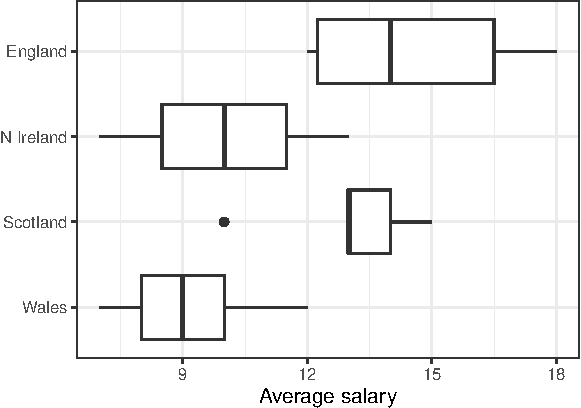
\includegraphics{05-anova_files/figure-pdf/fig-anova-samples-boxplots-1.pdf}

}

\caption{\label{fig-anova-samples-boxplots}Box plots of the average mean
salary data in Table Table~\ref{tbl-anova-samples-stats} indicate five
summary statistics: the median, two hinges (first and third quartiles)
and two whiskers (extending from the hinge to the most extreme data
point within \(1.5 \cdot \mathsf{IQR}\)).}

\end{figure}%

For \(\alpha = 0.05,\) we compute the upper-tail area \(F_{0.05}\)
i.e.~to the right of the critical value \(F_{0.05, 3, 16}\) by
consulting a statistical table or by using \texttt{R} to find
\(F_{0.05} = 3.2388715.\)

\begin{Shaded}
\begin{Highlighting}[]
\CommentTok{\# alt: qf(.05, df1 = 3, df2 = 16, lower.tail = FALSE)}
\FunctionTok{qf}\NormalTok{(}\DecValTok{1}\FloatTok{{-}.05}\NormalTok{, }\AttributeTok{df1 =} \DecValTok{4{-}1}\NormalTok{, }\AttributeTok{df2 =} \DecValTok{20{-}4}\NormalTok{) }
\end{Highlighting}
\end{Shaded}

\begin{verbatim}
[1] 3.238872
\end{verbatim}

The grand mean is \[
 \overline{x} = \frac{17 + 12 + 18 + \cdots + 8 + 7 + 9}{20} = 11.9\,,
\] and hence the variation among sample means is given by, \[
\begin{aligned}
 \mathsf{MSTr} &= \frac{1}{4-1} \left(m_1(\overline{x}_1 - \overline{x})^2 + \cdots + m_4 (\overline{x}_4 - \overline{x})^2\right) \\
 &= \left(6 (14.5-11.9)^2 + 4(10.0 - 11.9)^2 + 5(13.0-11.9)^2 + 5 ( 9.2 - 11.9)^2\right) / 3 \\
 &= 32.5 \,.
\end{aligned}
\] The mean square error is \[
 \begin{aligned}
 \mathsf{MSE} & = \frac{1}{20-4} \left((m_1 - 1)s_1^2 + \cdots (m_4-1)s_4^2\right)\\ 
  &= \frac{5(2.588)^2 + 3(2.582)^2 + 4(1.871)^2 + 4(1.924)^2}{16} \\
  &= 5.14366
 \end{aligned}
\] yielding the test statistic value \[
 F = \frac{\mathsf{MSTr}}{\mathsf{MSE}} = \frac{32.5}{5.14366} 
 = 6.3184581 \,.
\] Since \(F > F_\alpha\) we reject \(H_0.\) The data do not support the
hypothesis that the mean salaries in each nation are identical at the
\(5\%\) level.

\end{example}

\section{Confidence intervals}\label{sec-anova-ci}

In Section~\ref{sec-compare-means}, we gave a CI for comparing
population means involving the difference \(\mu_X - \mu_Y.\) In some
settings, we would like to give CIs for more complicated functions of
population means \(\mu_i.\) Let \[
 \theta = \sum_{i=1}^k c_i \mu_i\,,
\] for constants \(c_i.\) As we assume the \(X_ij\) are normally
distributed with \(\mathbf{E}[X_{ij}] = \mu_i\) and
\(\mathop{\mathrm{Var}}[X_{ij}] = \sigma^2,\) the estimator \[
 \widehat{\theta} = \sum_{i=1}^k c_i \overline{X}_{i}\,,
\] is normally distributed with \[
 \mathop{\mathrm{Var}}[\widehat{\theta}] = \sum_{i=1}^k c_i^2 \mathop{\mathrm{Var}}[\overline{X}_i] = \sigma^2 \sum_{i=1}^{k} \frac{c_i^2}{m_i}\,.
\] We estimate \(\sigma^2\) by the \(\mathsf{MSE}\) and standardise the
estimator to arrive at a \(\mathsf{t}\) variable \[
 \frac{\widehat{\theta} - \theta}{\widehat{\sigma}_{\widehat{\theta}}}\,,
\] where \(\widehat{\sigma}_{\widehat{\theta}}\) is the estimated
standard error of the estimator.

\begin{proposition}[]\protect\hypertarget{prp-ci-anova}{}\label{prp-ci-anova}

A \(100(1-\alpha)\%\) CI for \(\sum c_i \mu_i\) is given by \[
 \sum_{i=1}^k c_i \overline{x}_i \pm t_{\alpha/2, m-k} \sqrt{\mathsf{MSE} \sum_{i=1}^k \frac{c_i^2}{m_i}}\,.
\]

\end{proposition}

\begin{example}[]\protect\hypertarget{exm-anova-ci}{}\label{exm-anova-ci}

Determine a \(90\%\) CI for the difference in mean average salary for
councils in Scotland and England, based on the data available in
Table~\ref{tbl-anova-samples-stats}

For \(\alpha = 0.10,\) the critical value \(t_{0.05, 16} = 1.7458837\)
is found by looking in a table of \(\mathsf{t}\) critical values or by
using \texttt{R}:

\begin{Shaded}
\begin{Highlighting}[]
\CommentTok{\# alt: qt(0.1/2, 16, lower.tail = FALSE)}
\FunctionTok{qt}\NormalTok{(}\DecValTok{1}\FloatTok{{-}0.1}\SpecialCharTok{/}\DecValTok{2}\NormalTok{, }\AttributeTok{df =} \DecValTok{20} \SpecialCharTok{{-}} \DecValTok{4}\NormalTok{) }
\end{Highlighting}
\end{Shaded}

\begin{verbatim}
[1] 1.745884
\end{verbatim}

Then for the function \(\overline{x}_2 - \overline{x_1},\) \[
\begin{aligned}
(\overline{x}_{Eng} - \overline{x}_{Sco}) \pm& t_{0.05, 16} \sqrt{\mathsf{MSE}} \sqrt{\frac{1}{m_{Eng}} + \frac{1}{m_{Sco}}} \\
& = (14.5 - 13.0) \pm 1.7458837 \sqrt{5.14366} \sqrt{\frac{1}{6} + \frac{1}{5}} \\
& = 1.5 \pm 2.3976575\,.
\end{aligned}
\] Thus, a \(90\%\) confidence interval for \(\mu_{Eng} - \mu_{Sco}\) is
\((-0.8977\,, 3.898).\)

\end{example}

\begin{tcolorbox}[enhanced jigsaw, toprule=.15mm, leftrule=.75mm, colframe=quarto-callout-warning-color-frame, arc=.35mm, rightrule=.15mm, bottomrule=.15mm, coltitle=black, title=\textcolor{quarto-callout-warning-color}{\faExclamationTriangle}\hspace{0.5em}{Consider the following}, breakable, colbacktitle=quarto-callout-warning-color!10!white, bottomtitle=1mm, left=2mm, toptitle=1mm, titlerule=0mm, opacityback=0, opacitybacktitle=0.6, colback=white]

How does the result in Example~\ref{exm-anova-ci} compare to the
\(\mathsf{t}\) method in
Section~\ref{sec-compare-means-normpops-vars-unknown}?

\end{tcolorbox}

\chapter{Linear regression}\label{sec-linear-models}

Regression analysis allows us to study the relationship among two or
more rvs. Typically, we are interested in the relationship between a
response or dependent rv \(Y\) and a covariate \(X.\) The relationship
between \(X\) and \(Y\) will be explained through a regression function,
\[
 r(x) = \mathbf{E}[Y \mid X = x] = \int y f(y\mid x) dy \,.
\] In particular, we shall assume that \(r\) is linear,
\begin{equation}\phantomsection\label{eq-linear-regression-function}{
 r(x) = \beta_0 + \beta_1 x\,,
}\end{equation} and estimate the intercept \(\beta_0\) and slope
\(\beta_1\) of this linear model from sample data \[
 (Y_1, X_1), \dots, (Y_m, X_m) \sim F_{Y,X}\,.
\]

\begin{tcolorbox}[enhanced jigsaw, toprule=.15mm, leftrule=.75mm, colframe=quarto-callout-tip-color-frame, arc=.35mm, rightrule=.15mm, bottomrule=.15mm, coltitle=black, title=\textcolor{quarto-callout-tip-color}{\faLightbulb}\hspace{0.5em}{Alternative lingo}, breakable, colbacktitle=quarto-callout-tip-color!10!white, bottomtitle=1mm, left=2mm, toptitle=1mm, titlerule=0mm, opacityback=0, opacitybacktitle=0.6, colback=white]

The covariates \(X\) are also called predictor variables, explanatory
variables, independent variables, and/or features depending on who you
are talking to.

\end{tcolorbox}

\section{Simple linear regression
models}\label{sec-simple-linear-regression}

The simplest regression is when \(X_i\) is one-dimensional and \(r(x)\)
is linear as in Equation~\ref{eq-linear-regression-function}. A linear
regression posits the expected value of \(Y_i\) is a linear function of
the data \(X_i,\) but that \(Y\) deviates from its expected value by a
random amount for fixed \(x_i.\)

\begin{definition}[]\protect\hypertarget{def-linear-model}{}\label{def-linear-model}

The simple linear regression model relates a random response \(Y_i\) to
a set of independent variables \(X_i,\)
\begin{equation}\phantomsection\label{eq-linear-model}{
 Y_i = \beta_0 + \beta_1 X_i + \epsilon_i \,,
}\end{equation} where the intercept \(\beta_0\) and slope \(\beta_1\)
are unknown parameters and the random deviation or random error
\(\epsilon_i\) is a rv assumed to satisfy:

\begin{enumerate}
\def\labelenumi{\arabic{enumi}.}
\tightlist
\item
  \(\mathbf{E}[\epsilon_i \mid X_i = x_i] = 0,\)
\item
  \(\mathop{\mathrm{Var}}[\epsilon_i \mid X_i = x_i] = \sigma^2\) does
  not depend on \(x_i,\)
\item
  \(\epsilon_i\) and \(\epsilon_j\) are independent for
  \(i, j = 1, \dots, m.\)
\end{enumerate}

\end{definition}

From the assumptions on \(\epsilon_i,\) the linear model
Equation~\ref{eq-linear-model} implies \[
 \mathbf{E}[Y_i \mid X_i = x_i] = \beta_0 + \beta_1 x_i \,.
\] Thus, if \(\widehat{\beta}_0\) and \(\widehat{\beta}_1\) are
estimators of \(\beta_0\) and \(\beta_1,\) then the fitted line is \[
 \widehat{r}(x) = \widehat{\beta}_0 + \widehat{\beta}_1 x
\] and the predicted or fitted value
\(\widehat{Y}_i = \widehat{r}(X_i)\) is an estimator for
\(\mathbf{E}[Y_i \mid X_i = x_i].\) The residuals are defined to be
\begin{equation}\phantomsection\label{eq-ls-residuals}{
 \widehat{\epsilon}_i = Y_i - \widehat{Y}_i = Y_i - \left( \widehat{\beta}_0 + \widehat{\beta}_1 X_i \right) \,.
}\end{equation} The residual sums of squares,
\begin{equation}\phantomsection\label{eq-rss}{
 \mathsf{RSS} = \sum_{i=1}^m \widehat{\epsilon}_i^2\,,
}\end{equation} measures how well the regression line \(\widehat{r}\)
fits the data \((Y_1, X_1), \dots, (Y_m, X_m).\) The least squares
estimates of \(\widehat{\beta}_0\) and \(\widehat{\beta}_1\) are the
values that minimize the \(\mathsf{RSS}\) in Equation~\ref{eq-rss}.

\begin{theorem}[]\protect\hypertarget{thm-least-squares-estimates}{}\label{thm-least-squares-estimates}

The least squares estimates for \(\widehat{\beta}_1\) and
\(\widehat{\beta}_0\) are given by, respectively,
\begin{equation}\phantomsection\label{eq-ls-slope}{
 \widehat{\beta}_1 = \frac{\sum_{i=1}^m (X_i - \overline{X})(Y_i - \overline{Y})}{\sum_{i=1}^m (X_i - \overline{X})^2} = \frac{S_{xy}}{S_{xx}} \,,
}\end{equation} and
\begin{equation}\phantomsection\label{eq-ls-intercept}{
 \widehat{\beta}_0 = \overline{Y} - \widehat{\beta}_1 \overline{X}\,.
}\end{equation}

\end{theorem}

Equation~\ref{eq-rss} is a function of \(\widehat{\beta}_0\) and
\(\widehat{\beta}_1\) from the definition of the residuals
Equation~\ref{eq-ls-residuals}. Then Equation~\ref{eq-ls-slope} and
Equation~\ref{eq-ls-intercept} follow by equating the partial
derivatives of Equation~\ref{eq-rss} to zero. The \(\widehat{\beta}_0\)
and \(\widehat{\beta}_1\) are the unique solution to this linear system.

\begin{tcolorbox}[enhanced jigsaw, toprule=.15mm, leftrule=.75mm, colframe=quarto-callout-tip-color-frame, arc=.35mm, rightrule=.15mm, bottomrule=.15mm, coltitle=black, title=\textcolor{quarto-callout-tip-color}{\faLightbulb}\hspace{0.5em}{Alternative lingo}, breakable, colbacktitle=quarto-callout-tip-color!10!white, bottomtitle=1mm, left=2mm, toptitle=1mm, titlerule=0mm, opacityback=0, opacitybacktitle=0.6, colback=white]

The \(\mathsf{RSS}\) is sometimes referred to as the error sum of
squares and abbreviated \(\mathsf{SSE}\) (no, the order is not a typo).

\end{tcolorbox}

\begin{example}[]\protect\hypertarget{exm-linear-model-fit-residuals}{}\label{exm-linear-model-fit-residuals}

In Figure~\ref{fig-linear-model-fit} and
Figure~\ref{fig-linear-model-residuals}, we consider the \textbf{Cherry
Tree Data} (see Table~\ref{tbl-cherry-data}) and discussion). We fit a
least squares regression of timber volume (response variable) to the
tree's diameter (independent variable). As you would expect, the timber
yield increases with diameter.

The \texttt{R} code below can be used to calculate the least squares
regression and residuals.

\begin{Shaded}
\begin{Highlighting}[]
\FunctionTok{data}\NormalTok{(trees)}
\NormalTok{y }\OtherTok{\textless{}{-}}\NormalTok{ trees}\SpecialCharTok{$}\NormalTok{Volume}
\NormalTok{x }\OtherTok{\textless{}{-}}\NormalTok{ trees}\SpecialCharTok{$}\NormalTok{Girth }\CommentTok{\# NB: this is the diameter; data mislabeled!}
\NormalTok{fit }\OtherTok{\textless{}{-}} \FunctionTok{lm}\NormalTok{(y }\SpecialCharTok{\textasciitilde{}}\NormalTok{ x)}
\NormalTok{e }\OtherTok{\textless{}{-}} \FunctionTok{resid}\NormalTok{(fit)}
\NormalTok{yhat }\OtherTok{\textless{}{-}} \FunctionTok{predict}\NormalTok{(fit)}
\end{Highlighting}
\end{Shaded}

The \texttt{fit} data frame contains the estimates for
\(\widehat{\beta}_0\) and \(\widehat{\beta}_1\):

\begin{Shaded}
\begin{Highlighting}[]
\NormalTok{fit}\SpecialCharTok{$}\NormalTok{coefficients}
\end{Highlighting}
\end{Shaded}

\begin{verbatim}
(Intercept)           x 
 -36.943459    5.065856 
\end{verbatim}

Both Figure~\ref{fig-linear-model-fit} and
Figure~\ref{fig-linear-model-residuals} are scatter plots of the
observed values \(y.\) In Figure~\ref{fig-linear-model-fit}, the
regression line \(\widehat{y}\) is plotted along with the residuals
\(\widehat{\epsilon}.\) In Figure~\ref{fig-linear-model-residuals}, the
sample mean \(\overline{y}\) is plotted together with the deviations
\(y - \overline{y}.\)

\end{example}

\begin{figure}

\centering{

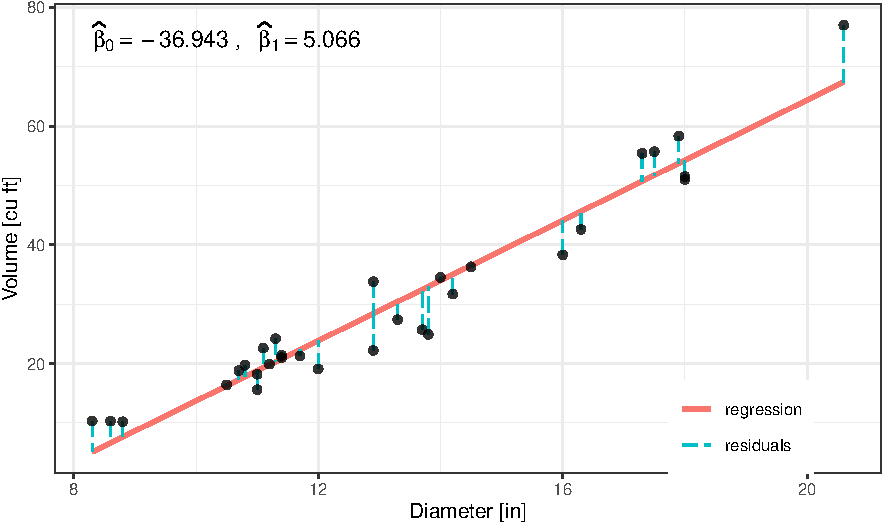
\includegraphics{06-linear-models_files/figure-pdf/fig-linear-model-fit-1.pdf}

}

\caption{\label{fig-linear-model-fit}Linear regression (or least squares
fit) of Volume to Diameter from the \textbf{Cherry Tree Data}. The
vertical bars between the observed data point and the regression line
indicate the error in the fit (the least squares residual). The
residuals are squared and summed to yield the \(\mathsf{RSS}\) (alt:
\(\mathsf{SSE}\)).}

\end{figure}%

\begin{figure}

\centering{

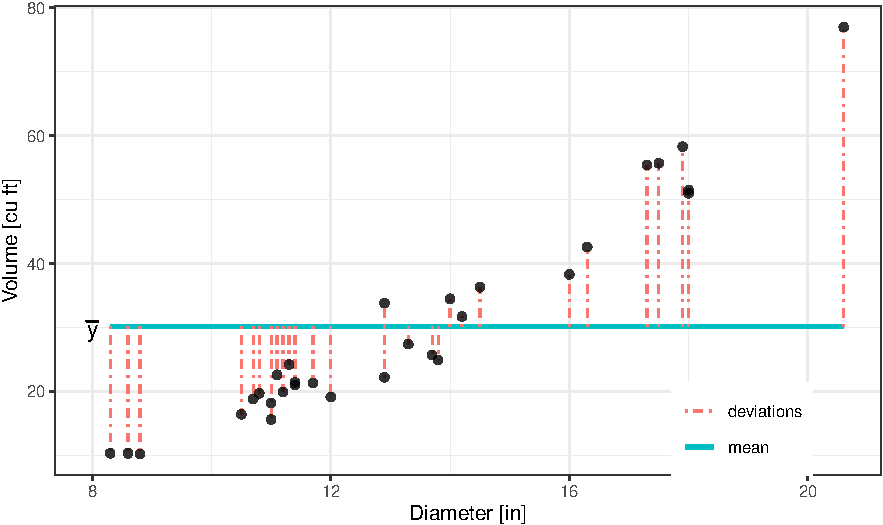
\includegraphics{06-linear-models_files/figure-pdf/fig-linear-model-residuals-1.pdf}

}

\caption{\label{fig-linear-model-residuals}The deviations about the
sample mean \(\overline{y}.\) The sum of the squared deviations or
\(\mathsf{SST}\) (total sum of squares) is a measure of the total
variation in the observations.}

\end{figure}%

\section{\texorpdfstring{Estimating \(\sigma^2\) for linear
regressions}{Estimating \textbackslash sigma\^{}2 for linear regressions}}\label{sec-ls-estimate-var}

The parameter \(\sigma^2\) (the variance of the random deviation)
determines the variability in the regression model.

\begin{theorem}[]\protect\hypertarget{thm-least-squares-var-estimate}{}\label{thm-least-squares-var-estimate}

An unbiased estimate of \(\sigma^2\) is given by
\begin{equation}\phantomsection\label{eq-least-squares-var-estimate}{
 \widehat{\sigma}^2 = s^2 = \frac{\mathsf{RSS}}{m-2} = \frac{1}{m-2} \sum_{i=1}^m (y_i - \widehat{y}_i)^2\,.
}\end{equation}

\end{theorem}

In Figure~\ref{fig-linear-model-sigma-large-v-small}, we present a least
squares regression of timber volume on both tree diameter and height
(for the \textbf{Cherry Tree Data}). As expected, the regressions
indicate the volume increases with both covariates. Estimates for the
variance of the random deviation
Equation~\ref{eq-least-squares-var-estimate} in both regression models,
\(\sigma_{D}^2\) and \(\sigma_{H}^2,\) respectively, are computed to be
\(s^2_{D} = 18.08\) and \(s^2_{H} = 179.48.\) Thus, we see that small
variances lead to observations of \((x_i, y_i)\) that sit tightly around
the regression line, in contrast to large variances that lead to a large
cloud of points.

\begin{figure}

\centering{

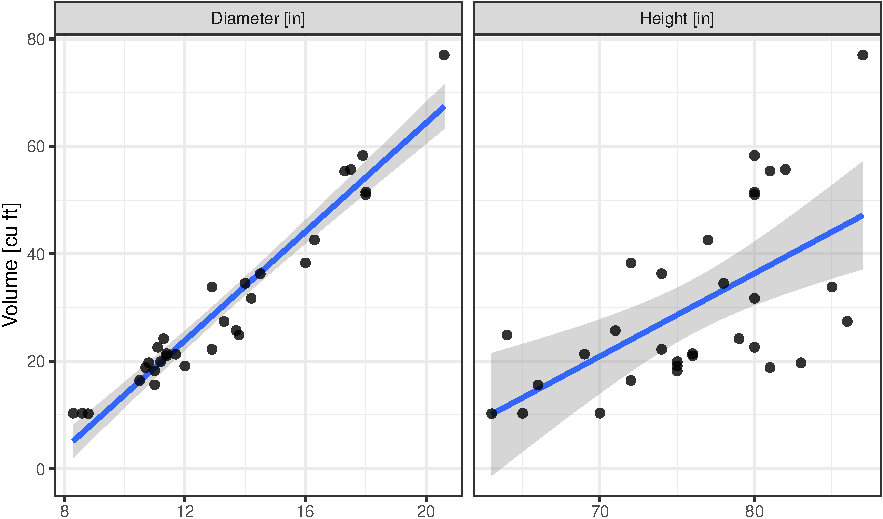
\includegraphics{06-linear-models_files/figure-pdf/fig-linear-model-sigma-large-v-small-1.pdf}

}

\caption{\label{fig-linear-model-sigma-large-v-small}For the
\textbf{Cherry Tree Data}, we estimate the variance to be
\(s^2_{D} = 18.08\) (for Diameter) and \(s^2_{H} = 179.48\) (for
Height); small variances lead to observations of \((x_i, y_i)\) that sit
tightly around the regression line, in contrast to large variances that
lead to a large cloud of points.}

\end{figure}%

\begin{tcolorbox}[enhanced jigsaw, toprule=.15mm, leftrule=.75mm, colframe=quarto-callout-warning-color-frame, arc=.35mm, rightrule=.15mm, bottomrule=.15mm, coltitle=black, title=\textcolor{quarto-callout-warning-color}{\faExclamationTriangle}\hspace{0.5em}{Why do we lose two degrees of freedom?}, breakable, colbacktitle=quarto-callout-warning-color!10!white, bottomtitle=1mm, left=2mm, toptitle=1mm, titlerule=0mm, opacityback=0, opacitybacktitle=0.6, colback=white]

In Theorem~\ref{thm-least-squares-var-estimate}, the number in the
denominator is the df associated with the \(\mathsf{RSS}\) and \(s^2.\)
To calculate \(\mathsf{RSS},\) you must estimate two parameters
\(\beta_0\) and \(\beta_1,\) which results in the loss of two df. Hence
the \(m-2.\)

\end{tcolorbox}

We note to make inferences, the statistic \[
 S^2 = \frac{\mathsf{RSS}}{m-2}
\] is an unbiased estimator or \(\sigma^2\) and the random variable \[
 \frac{(m-2) S^2}{\sigma^2} \sim \chi^2(m-2)\,.
\] Moreover, the statistic \(S^2\) is independent of both
\(\widehat{\beta}_0\) and \(\widehat{\beta}_1.\)

\section{Inferences for least-squares
parameters}\label{sec-inference-ls}

If \(\epsilon_i\) in Equation~\ref{eq-linear-model} is assumed to be
normally distributed, then we can derive the sampling distributions of
the estimators \(\widehat{\beta}_0\) and \(\widehat{\beta}_1.\) Hence,
we can use these sampling distributions to make inferences about the
parameters \(\beta_0\) and \(\beta_1.\)

Provided iid \(\epsilon_i \mid X_i \sim \mathsf{N}(0, \sigma^2),\) the
least-squares estimators possess the following properties.

\begin{enumerate}
\def\labelenumi{\arabic{enumi}.}
\tightlist
\item
  Both \(\widehat{\beta}_0\) and \(\widehat{\beta}_1\) are normally
  distributed.
\item
  Both \(\widehat{\beta}_0\) and \(\widehat{\beta}_1\) are unbiased,
  i.e., \(\mathbf{E}[\widehat{\beta}_i] = \beta_i\) for \(i = 0,1.\)
\item
  \(\mathop{\mathrm{Var}}[\widehat{\beta}_0] = c_{00} \sigma^2\) where
  \(c_{00} = \sum_{i=1}^m x_i^2 / (m S_{xx}).\)
\item
  \(\mathop{\mathrm{Var}}[\widehat{\beta}_1] = c_{11} \sigma^2\) where
  \(c_{11} = 1/S_{xx}.\)
\item
  \(\mathop{\mathrm{Cov}}[\widehat{\beta}_0, \widehat{\beta}_1] = c_{01} \sigma^2\)
  where \(c_{01} = - \overline{x} / S_{xx}.\)
\end{enumerate}

These properties can be determined by working directly from
Equation~\ref{eq-ls-slope} and Equation~\ref{eq-ls-intercept}.

\begin{proposition}[]\protect\hypertarget{prp-htest-ls-betas}{}\label{prp-htest-ls-betas}

Consider \(H_0 : \beta_i = \beta_{i0}.\) The test statistic is
\begin{equation}\phantomsection\label{eq-htest-ls-betas-statistic}{
 T = \frac{\widehat{\beta}_i - \beta_{i0}}{S\sqrt{c_{ii}}} \,.
}\end{equation}

For a hypothesis test at level \(\alpha,\) we use the following
procedure:

If \(H_a : \beta_i > \beta_{i0},\) then \(P\)-value is the area under
\(\mathsf{t}(m-2)\) to the right of \(t.\)

If \(H_a : \beta_i < \beta_{i0},\) tthen \(P\)-value is the area under
\(\mathsf{t}(m-2)\) to the left of \(t.\)

If \(H_a : \beta_i \neq \beta_{i0},\) then \(P\)-value is twice the area
under \(\mathsf{t}(m-2)\) to the right of \(|t|.\)

\end{proposition}

A confidence interval for \(\beta_i,\) based on the statistic
Equation~\ref{eq-htest-ls-betas-statistic}, can be given following the
procedures in Chapter~\ref{sec-inference-single-sample}.

\begin{proposition}[]\protect\hypertarget{prp-ci-ls-betas}{}\label{prp-ci-ls-betas}

A \(100(1-\alpha)\%\) CI for \(\beta_i\) is given by \[
 \widehat{\beta}_i \pm t_{\alpha/2, m-2} S \sqrt{c_{ii}} \,.
\]

\end{proposition}

\section{Correlation}\label{sec-correlation}

Let \((X_1, Y_1), \dots, (X_m, Y_m)\) denote a random sample from a
bivariate normal distribution with \(\mathbf{E}[X_i] = \mu_X,\)
\(\mathbf{E}[Y_i] = \mu_Y,\)
\(\mathop{\mathrm{Var}}[X_i] = \sigma_X^2,\)
\(\mathop{\mathrm{Var}}[Y_i] = \sigma_Y^2,\) and correlation coefficient
\(\rho.\) The sample correlation coefficient is given by,
\begin{equation}\phantomsection\label{eq-sample-correlation-statistic}{
 r = \frac{\sum_{i=1}^m (X_i - \overline{X})(Y_i - \overline{Y})}{\sqrt{\sum_{i=1}^m (X_i - \overline{X})^2 \sum_{i=1}^m (Y_i - \overline{Y})^2}}\,,
}\end{equation} which can be rewritten in terms of \(S_{xx},\)
\(S_{xy},\) and \(S_{yy}\): \[
 r = \frac{S_{xy}}{\sqrt{S_{xx}S_{yy}}} = \widehat{\beta}_1 \sqrt{\frac{S_{xx}}{S_{yy}}}\,,
\] using Equation~\ref{eq-ls-slope} and we see that \(r\) and
\(\widehat{\beta}_1\) have the same sign. A \(|r|\) close to \(1\) means
that the regression line is a good fit to the data, and, similarly, an
\(|r|\) close to \(0\) means a poor fit to the data. Note that the
correlation coefficient (and the least squares regression) are only
suitable for describing \emph{linear} relationships; a nonlinear
relationship can also yield \(r\) near zero (see
Figure~\ref{fig-linear-model-correlation}).

\begin{figure}

\centering{

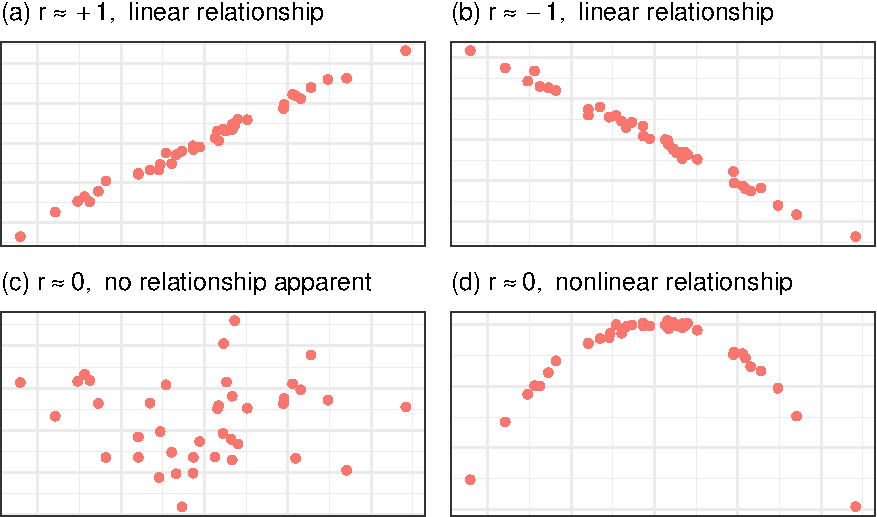
\includegraphics{06-linear-models_files/figure-pdf/fig-linear-model-correlation-1.pdf}

}

\caption{\label{fig-linear-model-correlation}Correlations range from
\(-1\) to \(1\) with \(|r|=1\) indicating a strong linear relationship
and \(r\) near zero indicating the absence of a linear relationship.}

\end{figure}%

\section{Prediction using linear
models}\label{prediction-using-linear-models}

Once a model is fit, it can be used to predict a value of \(y\) for a
given \(x.\) However, the model only gives the most likely value of
\(y\); a corresponding prediction interval is usually more appropriate.

\begin{proposition}[]\protect\hypertarget{prp-prediction-interval}{}\label{prp-prediction-interval}

A \(100(1-\alpha)\%\) prediction interval for an actual value of \(Y\)
when \(x = x^*\) is given by \[
 (\widehat{\beta}_0 + \widehat{\beta}_1 x^*) \pm t_{\alpha/2, m-2} S \sqrt{1 + \frac{1}{n} + \frac{(x^* - \overline{x})^2}{S_{xx}}} \,.
\]

\end{proposition}

\begin{tcolorbox}[enhanced jigsaw, toprule=.15mm, leftrule=.75mm, colframe=quarto-callout-warning-color-frame, arc=.35mm, rightrule=.15mm, bottomrule=.15mm, coltitle=black, title=\textcolor{quarto-callout-warning-color}{\faExclamationTriangle}\hspace{0.5em}{Prediction versus confidence intervals}, breakable, colbacktitle=quarto-callout-warning-color!10!white, bottomtitle=1mm, left=2mm, toptitle=1mm, titlerule=0mm, opacityback=0, opacitybacktitle=0.6, colback=white]

The prediction interval is different from the confidence interval for
expected \(Y.\) Note that the length of the \emph{confidence interval}
for \(\mathbf{E}[Y]\) when \(x=x^*\) is given by \[
 2 \cdot t_{\alpha/2} S  \sqrt{\frac{1}{n} + \frac{(x^* - \overline{x})^2}{S_{xx}}}
\] whereas the length for the \emph{prediction interval} of \(Y\) is \[
 2 \cdot t_{\alpha/2} S  \sqrt{1 + \frac{1}{n} + \frac{(x^* - \overline{x})^2}{S_{xx}}} \,.
\] Thus the prediction intervals for an actual value of \(Y\) are longer
than the confidence intervals for \(\mathbf{E}[Y]\) if both are
determined for the same value \(x^*.\)

\end{tcolorbox}

The linear model \[
 \mathbf{E}[ Y \mid X = x ] = \beta_0 + \beta_1 x \,, 
\] assumes that the conditional expectation of \(Y\) for a fixed value
of \(X\) is a linear function of the \(x\) value. If we assume that
\((X,Y)\) has a bivariate normal distribution, then \[
 \beta_1 = \frac{\sigma_Y}{\sigma_X} \rho \,,
\] and thus, for the simple hypothesis tests we have considered
(Table~\ref{tbl-htest-null-alt-forms}), statistical tests for
\(\beta_1\) and \(\rho\) are equivalent.

\chapter{Categorical data}\label{sec-categorical-data}

\section{Multinomial experiments}\label{multinomial-experiments}

Suppose we have a population divided into \(k > 2\) distinct categories.
We consider an experiment where we select \(m\) individuals (or objects)
from the population and categorise each. We denote the population
proportion in the \(i\)th category by \(p_i.\) If the sample size \(m\)
is much smaller than the population size \(M\) (so that the \(m\) trials
are independent), this experiment will be approximately
\emph{multinomial} with success probability \(p_i\) for each category,
\(i=1, \dots, k.\)

Before the experiment is performed, we denote the number (or count) of
the trials resulting in category \(i\) by the rv \(N_i.\) The expected
number of trails that result in category \(i\) is given by
\begin{equation}\phantomsection\label{eq-mean-count-multinomial}{
\mathbf{E}[N_i] = m p_i\,, \quad i=1, \dots, k\,.
}\end{equation} After the experiment is performed, we denote the
corresponding observed value by \(n_i.\) Since the trials result in
distinct categories, \[
\sum_{i=1}^k N_i = \sum_{i=1}^{k} n_i = m \,,
\] which indicates that, for a given \(m,\) we only need to observe
\(k-1\) of the variables to be able to work out what the \(k\)th
variable should be.

\section{Goodness-of-fit for a single
factor}\label{sec-goodness-of-fit-tests}

We are interested in making inferences about the proportion parameters
\(p_i.\) Specifically, we will consider the null hypothesis,
\begin{equation}\phantomsection\label{eq-null-multinomial}{
H_0 : p_1 = p_{10}\,, p_2 = p_{20}\,, \cdots\,, p_k = p_{k0}\,,
}\end{equation} that completely specifies a value \(p_{i0}\) for each
\(p_i.\) The alternative hypothesis \(H_a\) will state that \(H_0\) is
not true, i.e., that at least one \(p_i\) is different from the value
\(p_{i0}\) claimed under the null \(H_0.\)

\begin{tcolorbox}[enhanced jigsaw, toprule=.15mm, leftrule=.75mm, colframe=quarto-callout-warning-color-frame, arc=.35mm, rightrule=.15mm, bottomrule=.15mm, coltitle=black, title=\textcolor{quarto-callout-warning-color}{\faExclamationTriangle}\hspace{0.5em}{Notation}, breakable, colbacktitle=quarto-callout-warning-color!10!white, bottomtitle=1mm, left=2mm, toptitle=1mm, titlerule=0mm, opacityback=0, opacitybacktitle=0.6, colback=white]

Here for \(i=1, \dots, k\) we use the notation \(p_{i0}\) to denote the
value of \(p_i\) claimed under the null hypothesis.

\end{tcolorbox}

Provided the null hypothesis in Equation~\ref{eq-null-multinomial} is
true, the expected values Equation~\ref{eq-mean-count-multinomial} can
be written in terms of the expected frequencies, \[
 \mathbf{E}[N_i] = m p_{i0}\,, \quad i=1,\dots,k\,.
\] Often the \(n_i,\) referred to as the observed cell counts, and the
corresponding \(m p_{i0},\) referred to as the expected cell counts, are
tabulated, for example, as in Table~\ref{tbl-cell-counts}.

\begin{longtable}[]{@{}llllll@{}}
\caption{Observed and expected cell
counts.}\label{tbl-cell-counts}\tabularnewline
\toprule\noalign{}
Category & \(i=1\) & \(i=2\) & \(\cdots\) & \(i=k\) & Row total \\
\midrule\noalign{}
\endfirsthead
\toprule\noalign{}
Category & \(i=1\) & \(i=2\) & \(\cdots\) & \(i=k\) & Row total \\
\midrule\noalign{}
\endhead
\bottomrule\noalign{}
\endlastfoot
Observed & \(n_1\) & \(n_2\) & \(\cdots\) & \(n_k\) & \(m\) \\
Expected & \(mp_{10}\) & \(mp_{20}\) & \(\cdots\) & \(mp_{k0}\) &
\(m\) \\
\end{longtable}

The test procedure assesses the discrepancy between the value of the
observed and expected cell counts. This discrepancy, or goodness of fit,
is measured by the squared deviations divided by the expected count.

\begin{tcolorbox}[enhanced jigsaw, toprule=.15mm, leftrule=.75mm, colframe=quarto-callout-tip-color-frame, arc=.35mm, rightrule=.15mm, bottomrule=.15mm, coltitle=black, title=\textcolor{quarto-callout-tip-color}{\faLightbulb}\hspace{0.5em}{Why divide by expected cell counts?}, breakable, colbacktitle=quarto-callout-tip-color!10!white, bottomtitle=1mm, left=2mm, toptitle=1mm, titlerule=0mm, opacityback=0, opacitybacktitle=0.6, colback=white]

The division by the expected cell counts accounts for possible
differences in the relative magnitude of the observed/expected counts.

\end{tcolorbox}

\begin{theorem}[]\protect\hypertarget{thm-multinomial-experiment}{}\label{thm-multinomial-experiment}

For \(m p_i \geq 5\) for \(i = 1, \dots, k,\) the rv \[
 V = \sum_{i=1}^k \frac{(N_i - m p_i)^2}{m p_i} \quad \sim \chi^2(k-1)\,,
\] that is, \(V\) has approximately a \(\chi^2\) distribution with
\(\nu = k-1\) df.

\end{theorem}

\begin{proposition}[]\protect\hypertarget{prp-htest-multinomial}{}\label{prp-htest-multinomial}

Consider the null \[
H_0 : p_1 = p_{10}, p_2 = p_{20}, \cdots, p_k = p_{k0}\,,
\] and the alternative \[
H_a : p_i \neq p_{i0}\; \text{for at least one}\; i\,.
\] The test statistic is \[
 V = \sum_{i=1}^k \frac{(N_i - m p_{i0})^2}{m p_{i0}}\,.
\] As a rule of thumb, provided \(m p_{i0} \geq 5\) for all
\(i = 1, \dots, k,\) then the \(P\)-value is the area under
\(\chi^2(k-1)\) to the right of \(v.\)

\end{proposition}

If \(m p_{i0} < 5\) for some \(i\) then it may be possible to combine
the categories such that the new categorizations satisfy the assumptions
of Proposition~\ref{prp-htest-multinomial}.

\begin{tcolorbox}[enhanced jigsaw, toprule=.15mm, leftrule=.75mm, colframe=quarto-callout-warning-color-frame, arc=.35mm, rightrule=.15mm, bottomrule=.15mm, coltitle=black, title=\textcolor{quarto-callout-warning-color}{\faExclamationTriangle}\hspace{0.5em}{What about partial information?}, breakable, colbacktitle=quarto-callout-warning-color!10!white, bottomtitle=1mm, left=2mm, toptitle=1mm, titlerule=0mm, opacityback=0, opacitybacktitle=0.6, colback=white]

Things are much more complicated if the category probabilities are not
entirely specified.

\end{tcolorbox}

\section{Test for the independence of
factors}\label{test-for-the-independence-of-factors}

In Section~\ref{sec-goodness-of-fit-tests}, we considered categorising a
population into a single factor. We now consider a single population
where each individual is categorised into two factors with \(I\)
distinct categories for the first factor and \(J\) distinct categories
for the second factor. Each individual from the population belongs to
exactly one of the \(I\) categories of the first factor and exactly one
of the \(J\) categories of the second factor. We want to determine
whether or not there is any dependency between the two factors.

For a sample of \(m\) individuals, we denote by \(n_{ij}\) the count of
the \(m\) samples that fall both in category \(i\) of the first factor
and category \(j\) of the second factor, for \(i = 1, \dots, I\) and
\(j = 1, \dots, J.\) A contingency table with \(I\) rows and \(J\)
columns (i.e., \(IJ\) cells) will be used to record the \(n_{ij}\)
counts (in an obvious way). Let \(p_{ij}\) be the proportion of
individuals in the population who belong in category \(i\) of factor 1
and category \(j\) of factor \(2.\) Then, the probability that a
randomly selected individual falls in category \(i\) of factor 1 is
found by summing over all \(j\): \[
p_{i} = \sum_{j=1}^J p_{ij}\,,
\] and likewise, the probability that a randomly selected individual
falls in category \(j\) of factor 2 is found by summing over all \(i\):
\[
p_{j} = \sum_{i=1}^I p_{ij}\,.
\] The null hypothesis that we will be interested in adopting is
\begin{equation}\phantomsection\label{eq-null-two-factor}{
H_0 : p_{ij} = p_{i} \cdot p_{j} \; \forall (i,j)\,,
}\end{equation} that is, an individual's category in factor 1 is
independent of the category in factor 2.

Following the same program as for the single category goodness-of-fit
test, we note that assuming the null hypothesis
Equation~\ref{eq-null-two-factor} is true, then the expected count in
cell \(i,j\) is \[
 \mathbf{E}[N_{ij}] = m p_{ij} = m p_{i} p_{j}\,;
\] and we estimate \(p_i\) and \(p_j\) by the appropriate sample
proportion: \[
\widehat{p}_i = \frac{n_i}{m}\,, \qquad n_i = \sum_{j} n_{ij} \quad \text{(row totals)}\,,
\] and \[
\widehat{p}_j = \frac{n_j}{m}\,, \qquad n_j = \sum_{i} n_{ij}\quad \text{(column totals)}\,.
\] Thus, the expected cell count is given by \[
\widehat{e}_{ij} = m \widehat{p}_i \widehat{p}_j = \frac{n_i n_j}{m}\,,
\] and we assess the goodness of fit between the observed cell count
\(n_ij\) and the expected cell count \(\widehat{e}_ij.\)

\begin{proposition}[]\protect\hypertarget{prp-independence-test}{}\label{prp-independence-test}

Assume the null hypothesis \[
H_0 : p_{ij} = p_i p_j \; \text{for all } i=1, \dots, I\,, j=1, \dots, J\,,
\] against the alternative hypothesis \[
H_a : H_0 \;\text{is not true}\,. 
\] The test statistic is \[
V = \sum_{i=1}^I \sum_{j=1}^J \frac{(N_{ij} - \widehat{e}_{ij})^2}{\widehat{e}_{ij}} \,.
\] As a rule of thumb, provided \(\widehat{e}_{ij} \geq 5\) for all
\(i,j\) and when \(H_0\) is true, then the test statistic has
approximately a \(\chi^2(\nu)\) distribution with \(\nu = (I-1)(J-1)\)
df. For a hypothesis test at level \(\alpha,\) the procedure is
upper-tailed, and the \(P\)-value is the area under \(\chi^2(\nu)\) to
the right of \(v.\)

\end{proposition}

\begin{tcolorbox}[enhanced jigsaw, toprule=.15mm, leftrule=.75mm, colframe=quarto-callout-tip-color-frame, arc=.35mm, rightrule=.15mm, bottomrule=.15mm, coltitle=black, title=\textcolor{quarto-callout-tip-color}{\faLightbulb}\hspace{0.5em}{Alternative lingo}, breakable, colbacktitle=quarto-callout-tip-color!10!white, bottomtitle=1mm, left=2mm, toptitle=1mm, titlerule=0mm, opacityback=0, opacitybacktitle=0.6, colback=white]

Contingency is just another word for dependency in the context of
goodness-of-fit tables.

\end{tcolorbox}

\chapter{Quality control}\label{sec-quality-control}

Quality control is an area of applied statistics that makes
interventions to maintain or improve the outcome of industrial
processes. Random variations in output processes might negatively impact
the quality of a product. We want to identify the sources of random
output-process variations that might have \emph{assignable causes}.
Control charts are a tool that helps us to recognise when industrial
processes are no longer controlled so that one might then seek to
identify assignable causes.

\section{Control charts}\label{sec-control-charts}

The essential elements of control charting involve specifying a control
region and then analysing time-series data. We will specify a baseline
value along with an upper and lower control limit and assume that a
process is under control unless a test statistic suggests otherwise. To
construct a control chart, one collects data about a process at fixed
points of time and calculates the running value of a quality statistic.
Suppose the quality statistic exceeds the upper or lower control limits.
In that case, the process is deemed out of control, and the product
quality is assumed to be negatively impacted.

\begin{tcolorbox}[enhanced jigsaw, toprule=.15mm, leftrule=.75mm, colframe=quarto-callout-important-color-frame, arc=.35mm, rightrule=.15mm, bottomrule=.15mm, coltitle=black, title=\textcolor{quarto-callout-important-color}{\faExclamation}\hspace{0.5em}{Default position}, breakable, colbacktitle=quarto-callout-important-color!10!white, bottomtitle=1mm, left=2mm, toptitle=1mm, titlerule=0mm, opacityback=0, opacitybacktitle=0.6, colback=white]

The default position adopted for quality control will be reminiscent of
hypothesis testing: ``assume that a process is under control unless a
test statistic suggests otherwise.''

\end{tcolorbox}

The process of creating a control chart is best illustrated through an
extended example, like Example~\ref{exm-qc-three-sigma} provided below.

\begin{example}[]\protect\hypertarget{exm-qc-three-sigma}{}\label{exm-qc-three-sigma}

Here we consider the typical \(3 \sigma\) control charting for a process
mean \(\overline{X}\) based on estimated parameters. That is, we assume
the generating process \(X\) is normally distributed with unknown
parameters \(\mu\) and \(\sigma^2\). We seek to estimate the mean
\(\overline{X}\). Our control region is specified to be three standard
deviations; the process is in control if it remains within three
standard deviations of a baseline value.

\begin{tcolorbox}[enhanced jigsaw, toprule=.15mm, leftrule=.75mm, colframe=quarto-callout-note-color-frame, arc=.35mm, rightrule=.15mm, bottomrule=.15mm, coltitle=black, title=\textcolor{quarto-callout-note-color}{\faInfo}\hspace{0.5em}{Note \ref*{nte-beer}: Beer Production Data}, breakable, colbacktitle=quarto-callout-note-color!10!white, bottomtitle=1mm, left=2mm, toptitle=1mm, titlerule=0mm, opacityback=0, opacitybacktitle=0.6, colback=white]

\quartocalloutnte{nte-beer} 

The \textbf{Beer Production Data} contains measurements of the features
OG, ABV, pH, and IBU for \(50\) batches of each of three types of
product (Premium Lager, IPA, and Light Lager).

\begin{Shaded}
\begin{Highlighting}[]
\NormalTok{beer }\SpecialCharTok{|\textgreater{}} \FunctionTok{glimpse}\NormalTok{()}
\end{Highlighting}
\end{Shaded}

\begin{verbatim}
Rows: 150
Columns: 6
$ Batch_Id <dbl> 1, 2, 3, 4, 5, 6, 7, 8, 9, 10, 11, 12, 13, 14, 15, 16, 17, 18, 19, 20, ~
$ OG       <dbl> 5.1, 4.9, 4.7, 4.6, 5.0, 5.4, 4.6, 5.0, 4.4, 4.9, 5.4, 4.8, 4.8, 4.3, 5~
$ ABV      <dbl> 3.5, 3.0, 3.2, 3.1, 3.6, 3.9, 3.4, 3.4, 2.9, 3.1, 3.7, 3.4, 3.0, 3.0, 4~
$ pH       <dbl> 1.4, 1.4, 1.3, 1.5, 1.4, 1.7, 1.4, 1.5, 1.4, 1.5, 1.5, 1.6, 1.4, 1.1, 1~
$ IBU      <dbl> 9.0, 10.0, 7.0, 9.0, 8.0, 7.7, 7.4, 7.1, 6.8, 6.5, 6.2, 5.9, 5.6, 5.3, ~
$ Beer     <chr> "Premium Lager", "Premium Lager", "Premium Lager", "Premium Lager", "Pr~
\end{verbatim}

\end{tcolorbox}

Let's consider the Beer Production Data in Note~\ref{nte-beer}. We are
interested in the IPA's pH value, which influences saccharification. We
assume that three batches of IPA are produced per day, and we prepare
the data as follows.

\begin{Shaded}
\begin{Highlighting}[]
\NormalTok{ipa }\OtherTok{\textless{}{-}}\NormalTok{ beer }\SpecialCharTok{|\textgreater{}} 
 \FunctionTok{select}\NormalTok{(Batch\_Id, pH, Beer) }\SpecialCharTok{|\textgreater{}} 
 \FunctionTok{filter}\NormalTok{(Beer }\SpecialCharTok{==} \StringTok{"IPA"}\NormalTok{) }\SpecialCharTok{|\textgreater{}} 
 \FunctionTok{rename}\NormalTok{(}\AttributeTok{Day =}\NormalTok{ Batch\_Id)}

\NormalTok{m }\OtherTok{\textless{}{-}} \DecValTok{3}    \CommentTok{\# three batches per day}
\NormalTok{k }\OtherTok{\textless{}{-}} \DecValTok{16}   \CommentTok{\# number of days}
\NormalTok{ipa}\SpecialCharTok{$}\NormalTok{Day[}\DecValTok{1}\SpecialCharTok{:}\NormalTok{(m}\SpecialCharTok{*}\NormalTok{k)] }\OtherTok{\textless{}{-}} \FunctionTok{rep}\NormalTok{(}\DecValTok{1}\SpecialCharTok{:}\NormalTok{k, }\AttributeTok{each =}\NormalTok{ m)}
\NormalTok{ipa }\OtherTok{\textless{}{-}}\NormalTok{ ipa[}\DecValTok{1}\SpecialCharTok{:}\NormalTok{(m}\SpecialCharTok{*}\NormalTok{k),]}
\end{Highlighting}
\end{Shaded}

The prepared data, \texttt{ipa}, is summarized in the
Table~\ref{tbl-qc-beer-data}.

\begin{Shaded}
\begin{Highlighting}[]
\NormalTok{ipa\_stat }\OtherTok{\textless{}{-}}\NormalTok{ ipa }\SpecialCharTok{|\textgreater{}} 
 \FunctionTok{group\_by}\NormalTok{(Day) }\SpecialCharTok{|\textgreater{}} 
 \FunctionTok{summarise}\NormalTok{(}\AttributeTok{obs =} \FunctionTok{list}\NormalTok{(pH), }\AttributeTok{mean =} \FunctionTok{signif}\NormalTok{(}\FunctionTok{mean}\NormalTok{(pH), }\AttributeTok{digits =} \DecValTok{4}\NormalTok{), }
           \AttributeTok{sd =} \FunctionTok{signif}\NormalTok{(}\FunctionTok{sd}\NormalTok{(pH), }\AttributeTok{digits =} \DecValTok{4}\NormalTok{), }\AttributeTok{range =} \FunctionTok{max}\NormalTok{(pH) }\SpecialCharTok{{-}} \FunctionTok{min}\NormalTok{(pH)) }
\NormalTok{ipa\_stat }\SpecialCharTok{|\textgreater{}} 
 \FunctionTok{kbl}\NormalTok{(}\AttributeTok{align =} \StringTok{"rcccc"}\NormalTok{, }\AttributeTok{booktabs =}\NormalTok{ T, }\AttributeTok{escape =}\NormalTok{ F) }\SpecialCharTok{|\textgreater{}}
 \FunctionTok{kable\_styling}\NormalTok{(}\AttributeTok{latex\_options =} \FunctionTok{c}\NormalTok{(}\StringTok{"striped"}\NormalTok{))}
\end{Highlighting}
\end{Shaded}

\begin{table}

\caption{\label{tbl-qc-beer-data}Observations and summary statistics for
the \textbf{Beer Production Data}.}

\centering{

\centering
\begin{tabular}[t]{rcccc}
\toprule
Day & obs & mean & sd & range\\
\midrule
\cellcolor{gray!10}{1} & \cellcolor{gray!10}{4.7, 4.5, 4.9} & \cellcolor{gray!10}{4.700} & \cellcolor{gray!10}{0.20000} & \cellcolor{gray!10}{0.4}\\
2 & 4.0, 4.6, 4.5 & 4.367 & 0.32150 & 0.6\\
\cellcolor{gray!10}{3} & \cellcolor{gray!10}{4.7, 3.3, 4.6} & \cellcolor{gray!10}{4.200} & \cellcolor{gray!10}{0.78100} & \cellcolor{gray!10}{1.4}\\
4 & 3.9, 3.5, 4.2 & 3.867 & 0.35120 & 0.7\\
\cellcolor{gray!10}{5} & \cellcolor{gray!10}{4.0, 4.7, 3.6} & \cellcolor{gray!10}{4.100} & \cellcolor{gray!10}{0.55680} & \cellcolor{gray!10}{1.1}\\
\addlinespace
6 & 4.4, 4.5, 4.1 & 4.333 & 0.20820 & 0.4\\
\cellcolor{gray!10}{7} & \cellcolor{gray!10}{4.5, 3.9, 4.8} & \cellcolor{gray!10}{4.400} & \cellcolor{gray!10}{0.45830} & \cellcolor{gray!10}{0.9}\\
8 & 4.0, 4.9, 4.7 & 4.533 & 0.47260 & 0.9\\
\cellcolor{gray!10}{9} & \cellcolor{gray!10}{4.3, 4.4, 4.8} & \cellcolor{gray!10}{4.500} & \cellcolor{gray!10}{0.26460} & \cellcolor{gray!10}{0.5}\\
10 & 5.0, 4.5, 3.5 & 4.333 & 0.76380 & 1.5\\
\addlinespace
\cellcolor{gray!10}{11} & \cellcolor{gray!10}{3.8, 3.7, 3.9} & \cellcolor{gray!10}{3.800} & \cellcolor{gray!10}{0.10000} & \cellcolor{gray!10}{0.2}\\
12 & 5.1, 4.5, 4.5 & 4.700 & 0.34640 & 0.6\\
\cellcolor{gray!10}{13} & \cellcolor{gray!10}{4.7, 4.4, 4.1} & \cellcolor{gray!10}{4.400} & \cellcolor{gray!10}{0.30000} & \cellcolor{gray!10}{0.6}\\
14 & 4.0, 4.4, 4.6 & 4.333 & 0.30550 & 0.6\\
\cellcolor{gray!10}{15} & \cellcolor{gray!10}{4.0, 3.3, 4.2} & \cellcolor{gray!10}{3.833} & \cellcolor{gray!10}{0.47260} & \cellcolor{gray!10}{0.9}\\
\addlinespace
16 & 4.2, 4.2, 4.3 & 4.233 & 0.05774 & 0.1\\
\bottomrule
\end{tabular}

}

\end{table}%

We first observe that the pH measurements are (at least approximately)
normal, as seen in the quantile-quantile plot in
Figure~\ref{fig-qc-beer-pH-norm}.

\begin{Shaded}
\begin{Highlighting}[]
\NormalTok{ipa }\SpecialCharTok{|\textgreater{}} \FunctionTok{ggplot}\NormalTok{(}\FunctionTok{aes}\NormalTok{(}\AttributeTok{sample =}\NormalTok{ pH)) }\SpecialCharTok{+} \FunctionTok{stat\_qq}\NormalTok{() }\SpecialCharTok{+} \FunctionTok{stat\_qq\_line}\NormalTok{()}
\end{Highlighting}
\end{Shaded}

\begin{figure}[H]

\centering{

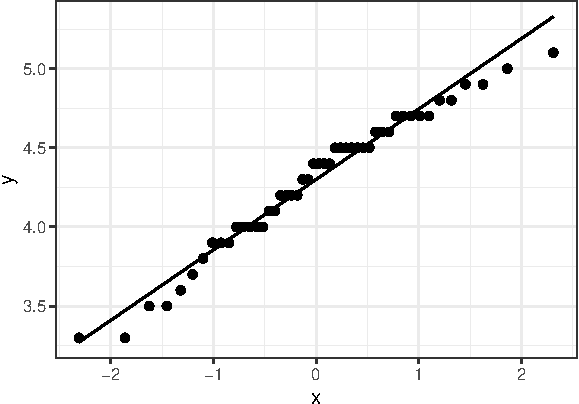
\includegraphics{08-quality-control_files/figure-pdf/fig-qc-beer-pH-norm-1.pdf}

}

\caption{\label{fig-qc-beer-pH-norm}Normal quantile-quantile plot of
observed pH measurements of the IPA batches.}

\end{figure}%

We consider the data for pH readings from three batches of IPA taken
over sixteen days (\(k = 16\)) presented in
Table~\ref{tbl-qc-beer-data}. The Table includes the sample mean per
day, \(\overline{x}\), the sample standard deviation, \(s\), and the
range of values per day, \(\max{x_i} - \min{x_i}\) (each based on
\(m=3\) batches).

We estimate the mean\\
\[
 \widehat{\mu} = \frac{1}{k} \sum_{i=1}^k \overline{x}_i \,,
\] by averaging the means found for the \(k\) days and, similarly,
estimating the mean of the sample standard deviation, \[
 \overline{s} = \frac{1}{k} \sum_{i=1}^k s_i\,,
\] by averaging the sample standard deviations for the \(k\) days. It
can be shown that \[
 \widehat{\sigma} = \frac{\overline{S}}{a_m} 
\] is an unbiased estimator of \(\sigma\) where \[
a_m = \frac{\sqrt{2} \Gamma(m/2)}{\sqrt{m-1}\Gamma\left((n-1)/2\right)}\,.
\] Thus, we compute the \(3\sigma\) upper and lower control limits,
respectively, \[
 \mathsf{UCL} = \widehat{\mu} + 3 \frac{\overline{s}}{a_m \sqrt{m}}
\] and \[
 \mathsf{LCL} = \widehat{\mu} - 3 \frac{\overline{s}}{a_m \sqrt{m}} \,.
\] The computations in \texttt{R} follow, along with the resulting
control chart in Figure~\ref{fig-qc-beer-control-chart}.

\begin{Shaded}
\begin{Highlighting}[]
\NormalTok{a }\OtherTok{\textless{}{-}} \ControlFlowTok{function}\NormalTok{(m)\{ }\FunctionTok{sqrt}\NormalTok{(}\DecValTok{2}\NormalTok{) }\SpecialCharTok{*} \FunctionTok{gamma}\NormalTok{(m}\SpecialCharTok{/}\DecValTok{2}\NormalTok{) }\SpecialCharTok{/}\NormalTok{ (}\FunctionTok{sqrt}\NormalTok{(m}\DecValTok{{-}1}\NormalTok{) }\SpecialCharTok{*} \FunctionTok{gamma}\NormalTok{((m}\DecValTok{{-}1}\NormalTok{)}\SpecialCharTok{/}\DecValTok{2}\NormalTok{)) \}}
\NormalTok{muhat }\OtherTok{=} \FunctionTok{sum}\NormalTok{(ipa\_stat}\SpecialCharTok{$}\NormalTok{mean) }\SpecialCharTok{/}\NormalTok{ k}
\NormalTok{sbar }\OtherTok{=} \FunctionTok{sum}\NormalTok{(ipa\_stat}\SpecialCharTok{$}\NormalTok{sd) }\SpecialCharTok{/}\NormalTok{ k}
\NormalTok{lcl }\OtherTok{=}\NormalTok{ muhat }\SpecialCharTok{{-}} \DecValTok{3}\SpecialCharTok{*}\NormalTok{sbar }\SpecialCharTok{/}\NormalTok{ (}\FunctionTok{a}\NormalTok{(m) }\SpecialCharTok{*} \FunctionTok{sqrt}\NormalTok{(m))}
\NormalTok{ucl }\OtherTok{=}\NormalTok{ muhat }\SpecialCharTok{+} \DecValTok{3}\SpecialCharTok{*}\NormalTok{sbar }\SpecialCharTok{/}\NormalTok{ (}\FunctionTok{a}\NormalTok{(m) }\SpecialCharTok{*} \FunctionTok{sqrt}\NormalTok{(m))}

\FunctionTok{ggplot}\NormalTok{(ipa\_stat, }\FunctionTok{aes}\NormalTok{(}\AttributeTok{x =}\NormalTok{ Day)) }\SpecialCharTok{+} \FunctionTok{geom\_point}\NormalTok{(}\FunctionTok{aes}\NormalTok{(}\AttributeTok{y =}\NormalTok{ mean)) }\SpecialCharTok{+} 
 \FunctionTok{geom\_hline}\NormalTok{(}\FunctionTok{aes}\NormalTok{(}\AttributeTok{yintercept =}\NormalTok{ muhat, }\AttributeTok{color =} \StringTok{"Mean"}\NormalTok{), }\AttributeTok{linewidth =}\NormalTok{ lsz) }\SpecialCharTok{+} 
 \FunctionTok{geom\_hline}\NormalTok{(}\FunctionTok{aes}\NormalTok{(}\AttributeTok{yintercept =}\NormalTok{ lcl, }\AttributeTok{color =} \StringTok{"LCL"}\NormalTok{), }\AttributeTok{linewidth =}\NormalTok{ lsz}\SpecialCharTok{*}\FloatTok{1.5}\NormalTok{) }\SpecialCharTok{+} 
 \FunctionTok{geom\_hline}\NormalTok{(}\FunctionTok{aes}\NormalTok{(}\AttributeTok{yintercept =}\NormalTok{ ucl, }\AttributeTok{color =} \StringTok{"UCL"}\NormalTok{), }\AttributeTok{linewidth =}\NormalTok{ lsz}\SpecialCharTok{*}\FloatTok{1.5}\NormalTok{) }\SpecialCharTok{+} \FunctionTok{ylab}\NormalTok{(}\StringTok{"pH"}\NormalTok{) }\SpecialCharTok{+} 
   \FunctionTok{theme}\NormalTok{(}\AttributeTok{legend.justification =} \FunctionTok{c}\NormalTok{(}\DecValTok{1}\NormalTok{,}\DecValTok{1}\NormalTok{), }\AttributeTok{legend.position =} \FunctionTok{c}\NormalTok{(}\FloatTok{0.9}\NormalTok{,}\FloatTok{0.9}\NormalTok{),}
         \AttributeTok{legend.title =} \FunctionTok{element\_blank}\NormalTok{(), }
         \AttributeTok{legend.box.margin =} \FunctionTok{margin}\NormalTok{(}\FunctionTok{c}\NormalTok{(}\DecValTok{4}\NormalTok{, }\DecValTok{4}\NormalTok{, }\DecValTok{4}\NormalTok{, }\DecValTok{4}\NormalTok{), }\AttributeTok{unit =} \StringTok{"pt"}\NormalTok{))}
\end{Highlighting}
\end{Shaded}

\begin{figure}[H]

\centering{

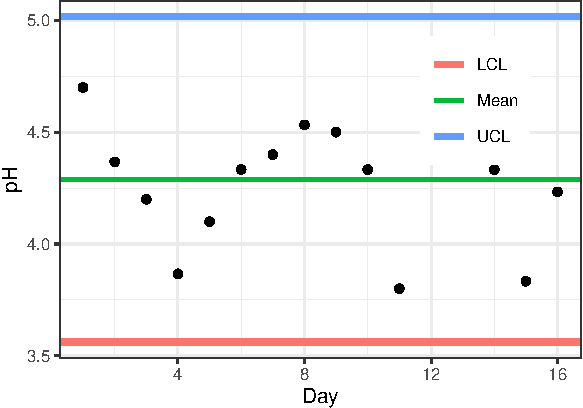
\includegraphics{08-quality-control_files/figure-pdf/fig-qc-beer-control-chart-1.pdf}

}

\caption{\label{fig-qc-beer-control-chart}The \(3\sigma\) control chart
illustrates that with respect to pH the brewing process is in-control
over the selected timeframe as the observations fall within the
\((\mathsf{LCL}, \mathsf{UCL})\) control interval.}

\end{figure}%

From Figure~\ref{fig-qc-beer-control-chart}, we observe for each day the
process is in-control as the observed mean pH values fall within the
control limits \((\mathsf{LCL}, \mathsf{UCL})\). If this were not the
case, our initial assumption that the process is in control would be
violated. The violation of the assumption would require that we seek to
identify an assignable cause for the variation. If a cause could be
identified, we would need to recompute our control limits with the
observations that were out of control removed.

\end{example}

\chapter*{References}\label{references}
\addcontentsline{toc}{chapter}{References}

\markboth{References}{References}

\begingroup
\raggedright

\phantomsection\label{refs}
\begin{CSLReferences}{1}{0}
\bibitem[\citeproctext]{ref-vanBelle:2008rt}
Belle, Gerald van. 2008. \emph{Statistical {R}ules of {T}humb}. Second.
Wiley Series in Probability and Statistics. Hoboken, NJ: John Wiley \&
Sons, Inc.

\bibitem[\citeproctext]{ref-Spiegelhalter:2020ps}
Spiegelhalter, David J. 2020. \emph{The {A}rt of {S}tatistics:
{L}earning from {D}ata}. London: Pelican Books.

\bibitem[\citeproctext]{ref-Wasserman:2013as}
Wasserman, Larry. 2004. \emph{All of {S}tatistics}. New York:
Springer-Verlag.

\end{CSLReferences}

\endgroup

\cleardoublepage
\phantomsection
\addcontentsline{toc}{part}{Appendices}
\appendix

\chapter*{Curated Content}\label{curated-content}
\addcontentsline{toc}{chapter}{Curated Content}

\markboth{Curated Content}{Curated Content}

Below we provide links to supplementary online material. Hopefully, some
of the items will inspire you to view the module material in a broader
context and lead to further investigations.

\section*{Investigation 1}\label{investigation-1}
\addcontentsline{toc}{section}{Investigation 1}

\markright{Investigation 1}

What is Statistics?

\begin{itemize}
\item
  \begin{description}
  \tightlist
  \item[Cambridge Ideas - Professor Risk]
  \url{https://www.youtube.com/watch?v=a1PtQ67urG4} \newline  Prof David
  Spiegelhalter (Cambridge University) discusses public understanding of
  risk. You may also be interested in reading
  (\citeproc{ref-Spiegelhalter:2020ps}{Spiegelhalter 2020}).
  \end{description}
\item
  \begin{description}
  \tightlist
  \item[The Joy of Statistics]
  \url{https://www.youtube.com/watch?v=jbkSRLYSojo} \newline  Prof Hans
  Rosling (Karolinska Institute and Gapminder Foundation) analyses data
  from 200 Countries over 200 Years in 4 Minutes - The Joy of Stats -
  BBC Four.
  \end{description}
\item
  \begin{description}
  \tightlist
  \item[Teach statistics before calculus!]
  \url{https://www.ted.com/talks/arthur_benjamin_teach_statistics_before_calculus}
  \newline  Prof Arthur Benjamin (Harvey Mudd College) argues that the
  pinnacle of math education is probability and statistics --- not
  calculus.
  \end{description}
\item
  \begin{description}
  \tightlist
  \item[Kaggle]
  \url{https://www.kaggle.com/} \newline Towards data science.

  \url{https://www.youtube.com/watch?v=TNzDMOg_zsw} \newline What's
  Kaggle?
  \end{description}
\end{itemize}

\section*{Investigation 2}\label{investigation-2}
\addcontentsline{toc}{section}{Investigation 2}

\markright{Investigation 2}

Defence against the dark arts.

\begin{itemize}
\item
  \begin{description}
  \tightlist
  \item[Three ways to spot bad statistics]
  \url{https://www.ted.com/talks/mona_chalabi_3_ways_to_spot_a_bad_statistic}
  \newline  Mona Chalabi (Data Journalist) discusses three ways to spot
  bad statistics.
  \end{description}
\end{itemize}

\begin{itemize}
\item
  \begin{description}
  \tightlist
  \item[Statistics Done Wrong]
  \url{https://www.statisticsdonewrong.com/} \newline  A book by Dr Alex
  Reinhart (Carnegie Mellon University).
  \end{description}
\item
  \begin{description}
  \tightlist
  \item[How to defend yourself against misleading statistics in the
  news]
  \url{https://www.youtube.com/watch?v=mJ63-bQc9Xg} \newline  Sanne
  Blauw (Journalist) discusses how the presentation of statistics can
  mislead.
  \end{description}
\end{itemize}

\section*{Investigation 3}\label{investigation-3}
\addcontentsline{toc}{section}{Investigation 3}

\markright{Investigation 3}

Data analysis and visualisation.

\begin{itemize}
\item
  \begin{description}
  \tightlist
  \item[The Grammar of Graphics]
  \url{https://www.youtube.com/watch?v=h-62NwWUI5c} \newline  What Makes
  A Good Visualisation? Rhys Jackson from RocketMill, a UK Digital
  Marketing Agency, gives a perspective on visualising data from a
  marketing perspective.

  \url{https://www.youtube.com/watch?v=kepKM7Z2O54} \newline  David
  Keyes (RStudio) discusses how the grammar of graphics underpins the
  \texttt{ggplot2} data visualization package in \texttt{R}.
  \end{description}
\item
  \begin{description}
  \tightlist
  \item[Same Stats, Different Graphs]
  \url{https://www.autodeskresearch.com/publications/samestats}
  \newline  Generating Datasets with Varied Appearance and Identical
  Statistics through Simulated Annealing (ACM SIGCHI Conference on Human
  Factors in Computing Systems) by Justin Matejka, George Fitzmaurice.
  \end{description}
\item
  \begin{description}
  \tightlist
  \item[Why do we so often use 0.05 for hypothesis testing?]
  \url{https://www.openintro.org/book/stat/why05/} \newline  In this
  online exercise, you will gain an improved understanding of what a
  significance level is, and why a value in the neighbourhood of 0.05 is
  reasonable as a default.
  \end{description}
\item
  \begin{description}
  \tightlist
  \item[Data visualisations]
  \url{https://flowingdata.com/} \newline  FlowingData blog by Nathan
  Yau.

  \url{https://fivethirtyeight.com/} \newline  FiveThirtyEight blog by
  Nate Silver.
  \end{description}
\item
  \begin{description}
  \tightlist
  \item[Storytelling with data]
  \url{http://www.storytellingwithdata.com/blog} \newline Blog with nice
  hints and tips for how to present data in tables, graphics, and
  visualisations.

  \url{https://community.storytellingwithdata.com/challenges}
  \newline Monthly challenge.
  \end{description}
\end{itemize}

\section*{Investigation 4}\label{investigation-4}
\addcontentsline{toc}{section}{Investigation 4}

\markright{Investigation 4}

Statistical paradoxes.

\begin{itemize}
\item
  \begin{description}
  \tightlist
  \item[How statistics can be misleading (TED-Ed)]
  \url{https://www.ted.com/talks/mark_liddell_how_statistics_can_be_misleading}
  \newline  Mark Liddell (Educator) discusses Simpson's Paradox in this
  TED-Ed animation.
  \end{description}
\item
  \begin{description}
  \tightlist
  \item[Low birth-weight paradox]
  \url{https://www.wikiwand.com/en/Low_birth-weight_paradox}
  \end{description}
\item
  \begin{description}
  \tightlist
  \item[Gambler's Fallacy]
  \url{https://www.youtube.com/watch?v=4eVluL-idkM} \newline  Prof Kelly
  Shue (Chicago Booth) discusses the gambler's fallacy.
  \end{description}
\end{itemize}

\section*{Investigation 5}\label{investigation-5}
\addcontentsline{toc}{section}{Investigation 5}

\markright{Investigation 5}

The law and interpreting statistics.

\begin{itemize}
\item
  \begin{description}
  \tightlist
  \item[How stats fool juries.]
  \url{https://youtu.be/kLmzxmRcUTo} \newline  Prof Peter Donnelly
  (Oxford University) discusses common mistakes in interpreting
  statistics.
  \end{description}
\end{itemize}

\begin{itemize}
\item
  \begin{description}
  \tightlist
  \item[Measurement Uncertainty Calculator (MUCalc)]
  \url{https://discovery.dundee.ac.uk/en/publications/measurement-uncertainty-calculator-mucalc}
  \newline  The Leverhulme Research Centre for Forensic Science
  Measurement Uncertainty Calculator (MUCalc) is an application for
  calculating measurement uncertainty in accordance with the standards
  of International Organization for Standardization ISO/IEC 17025.
  \end{description}
\item
  \begin{description}
  \tightlist
  \item[Prosecutor's fallacy]
  \url{https://www.wikiwand.com/en/Prosecutor\%27s_fallacy} \newline  A
  fallacy of statistical reasoning, typically used by a prosecutor to
  exaggerate the likelihood of guilt: because
  \(P(\text{hypothesis} \mid \text{evidence}) \neq P(\text{evidence} \mid \text{hypothesis})\)!
  \end{description}
\end{itemize}

\section*{Investigation 6}\label{investigation-6}
\addcontentsline{toc}{section}{Investigation 6}

\markright{Investigation 6}

Data-driven decision making in epidemiology.

\begin{itemize}
\item
  \begin{description}
  \tightlist
  \item[Project Tycho]
  \url{https://www.tycho.pitt.edu/} \newline  Digitized archival
  epidemiological data for the United States and the world.

  \url{https://www.youtube.com/watch?v=Kn9OJy1BPDo} \newline  An
  overview of the origins of project Tycho.
  \end{description}
\end{itemize}

\begin{itemize}
\item
  \begin{description}
  \tightlist
  \item[Our World in Data]
  \url{https://ourworldindata.org/} \newline  A project of the Oxford
  Martin School to make public health data, including progress in UN
  Sustainable Development Goals, available and accessible.
  \end{description}
\item
  \begin{description}
  \tightlist
  \item[Demographic Party Trick]
  \url{https://www.youtube.com/watch?v=2nDh8MQuS-Y} \newline  Prof Hans
  Rosling (Karolinska Institute and Gapminder Foundation) and Bill Gates
  seek to shed light on the true statistics of childhood vaccinations.
  \end{description}
\end{itemize}

\section*{Investigation 7}\label{investigation-7}
\addcontentsline{toc}{section}{Investigation 7}

\markright{Investigation 7}

Spurious correlations!

\begin{itemize}
\item
  \begin{description}
  \tightlist
  \item[The danger of mixing up causality and correlation]
  \url{https://www.youtube.com/watch?v=8B271L3NtAw} \newline  Prov
  Ionica Smeets (University of Leiden) discusses causality and
  correlation.
  \end{description}
\item
  \begin{description}
  \tightlist
  \item[Spurious correlations]
  \url{https://tylervigen.com/spurious-correlations} \newline  Tyler
  Vigen's site dedicated to spurious correlations.
  \end{description}
\item
  \begin{description}
  \tightlist
  \item[Cause \& Effect]
  \url{https://www.youtube.com/watch?v=lbODqslc4Tg}
  \newline  Correlation vs.~causality from the Clip from the 2010
  documentary ``Freakonomics: The Movie''.
  \end{description}
\end{itemize}

\section*{Investigation 8}\label{investigation-8}
\addcontentsline{toc}{section}{Investigation 8}

\markright{Investigation 8}

Data and Society: can data-driven and predictive modelling lead to a
better world? What are the ethics of mass data collection?

\begin{itemize}
\item
  \begin{description}
  \tightlist
  \item[Science behind the news: Predictive Policing]
  \url{https://www.youtube.com/watch?v=74_jreara3w} \newline  The Los
  Angeles Police Department is using a new tactic in their fight against
  crime called ``predictive policing.'' It's a computer program
  originally developed by a team at UCLA, including mathematician Andrea
  Bertozzi and anthropologist Jeff Brantingham. ``Science Behind the
  News'' is produced in partnership with NBC Learn. (Provided by the
  National Science Foundation \& NBC Learn)
  \end{description}
\item
  \begin{description}
  \tightlist
  \item[You should get paid for your data]
  \url{https://www.nytimes.com/video/opinion/100000006678020/data-privacy-jaron-lanier-2.html}
  \newline  Jaron Lanier (Computer Scientist and Author) discusses a
  compensation plan and data dignity.

  \url{https://www.ted.com/talks/jennifer_zhu_scott_why_you_should_get_paid_for_your_data}
  \newline  Jennifer Zhu Scott (Computer Scientist) also thinks you
  should get paid for your data.
  \end{description}
\item
  \begin{description}
  \tightlist
  \item[How tech companies deceive you into giving up your data and
  privacy]
  \url{https://www.ted.com/talks/finn_lutzow_holm_myrstad_how_tech_companies_deceive_you_into_giving_up_your_data_and_privacy}
  \newline  Finn Lützow-Holm Myrstad (Norwegian Consumer Council)
  discusses consumer protections and data collection.
  \end{description}
\item
  \begin{description}
  \tightlist
  \item[Your company's data could help end world hunger]
  \url{https://www.ted.com/talks/mallory_freeman_your_company_s_data_could_help_end_world_hunger}
  \newline Mallory Freeman (Data Scientist) discusses how to do the most
  good with data.
  \end{description}
\end{itemize}

\section*{Investigation 9}\label{investigation-9}
\addcontentsline{toc}{section}{Investigation 9}

\markright{Investigation 9}

Machine learning / big data.

\begin{itemize}
\item
  \begin{description}
  \tightlist
  \item[What is Machine Learning?]
  \url{https://www.youtube.com/watch?v=f_uwKZIAeM0}
  \newline  OxfordSparks discusses the topic of supervised learning
  algorithms and how machine learning is used all around us.
  \end{description}
\item
  \begin{description}
  \tightlist
  \item[Big Data (TED-Ed)]
  \url{https://www.youtube.com/watch?v=j-0cUmUyb-Y} \newline Tim Smith
  (educator) discusses the historical arc of big data in this TED-Ed
  animation.
  \end{description}
\item
  \begin{description}
  \tightlist
  \item[The human insights missing from big data]
  \url{https://www.ted.com/talks/tricia_wang_the_human_insights_missing_from_big_data}
  \newline  Tricia Wang (Ethnographer) discusses the human insights
  missing from big data.
  \end{description}
\item
  \begin{description}
  \tightlist
  \item[How we can find ourselves in data]
  \url{https://www.ted.com/talks/giorgia_lupi_how_we_can_find_ourselves_in_data}
  \newline Giorgia Lupi (Designer) discusses a humanistic approach to
  data and data visualization.
  \end{description}
\end{itemize}



\end{document}
